\documentclass[11pt,a4paper]{article}
\usepackage[T1]{fontenc}
\usepackage{lmodern}
\usepackage{graphicx}
\usepackage{amsmath,amssymb,bm,mathtools}
\usepackage{booktabs,tabularx,array,multirow}
\usepackage{setspace}
\usepackage{caption}
\usepackage{float}
\usepackage{titlesec}
\usepackage{geometry}
\usepackage{siunitx}
\usepackage{enumitem}
\usepackage{newunicodechar}
\newunicodechar{₀}{$_0$}
\usepackage{listings}
\usepackage{xcolor}
\usepackage[numbers,sort&compress]{natbib}
\usepackage{url}
\usepackage{hyperref}
\usepackage{tikz}
\usetikzlibrary{arrows.meta,positioning,shapes.geometric,fit,calc}
\usepackage{fancyhdr}
\usepackage{lastpage}
\usepackage{pdfpages}

\lstdefinestyle{mypython}{
    language=Python,
    basicstyle=\ttfamily\small,
    keywordstyle=\bfseries\color{blue},
    stringstyle=\color{teal},
    commentstyle=\color{gray}\itshape,
    numbers=left,
    numberstyle=\tiny\color{gray},
    stepnumber=1,
    numbersep=8pt,
    showstringspaces=false,
    breaklines=true,
    breakatwhitespace=true,
    tabsize=4,
    columns=fullflexible,keepspaces=true,
    frame=single,
    rulecolor=\color{gray},
    backgroundcolor=\color{white}
}

\def\BibTeX{{\rm B\kern-.05em{\sc i\kern-.025em b}\kern-.08em
    T\kern-.1667em\lower.7ex\hbox{E}\kern-.125emX}}

\geometry{a4paper,margin=1in}
\setstretch{1.2}
\hypersetup{colorlinks=true,linkcolor=blue,citecolor=blue,urlcolor=blue}
\sisetup{detect-all}

\newcommand{\teamnum}{1194}   % TEAM NUMBER (single place)
\pagestyle{fancy}
\fancyhf{}
\fancyhead[L]{Team \teamnum, Problem B}
\fancyhead[R]{Page \thepage\ of \pageref{LastPage}}
\renewcommand{\headrulewidth}{0.4pt}

\fancypagestyle{plain}{
    \fancyhf{}
    \fancyhead[L]{Team \teamnum, Problem B}
    \fancyhead[R]{Page \thepage\ of \pageref{LastPage}}
    \renewcommand{\headrulewidth}{0.4pt}
}

\begin{document}

% ===== PAGE 1: ONLY team number, problem letter, title, summary (<= 300 words) =====
\thispagestyle{plain}
\vspace*{0.3cm}
\begin{center}
  {\Large\bfseries Team \teamnum}\\[4pt]
  {\Large\bfseries Problem B}\\[16pt]
  {\LARGE\bfseries Bayesian Prediction of a Penalty Kick's Goal Entry Point from Two Early Observations}\\[18pt]
\end{center}

\begin{center}
  {\large\bfseries Abstract}
\end{center}
\vspace{2pt}
We predict where a penalty kick crosses the goal plane ($x=11$ m) from the ball's positions at 0.05 s and 0.10 s, and quantify the uncertainty. A layered model (gravity, quadratic drag, Magnus lift) is integrated with fourth-order Runge--Kutta, fitting the launch velocity to the observations. Because two positions give six numbers while the full model has seven unknowns, the problem is underdetermined, so we treat the prediction as Bayesian inference. Our main method draws 2000 combinations of drag, lift and spin axis from literature-based priors, fits the launch velocity for each, weights them by likelihood and propagates them to the goal, giving a best-estimate (weighted-mean) entry point and 68\,\%/95\,\% uncertainty ellipses. We test it on simulated penalties, including shots with richer physics and wind. On 300 test shots the median error is 26 cm (25 cm with richer physics), about half that of simpler extrapolations, and the 68\,\% and 95\,\% ellipses contain the true point in 69--70\,\% and 92--93\,\% of cases. For the given shot the ball most likely enters near $y=2.65\pm0.22$ m, $z=1.95\pm0.23$ m ($1\sigma$; posterior mean, with the posterior mode at $y=2.55$ m), inside the goal with probability 0.99; the whole ball clears the frame with probability 0.95. The height is robust, but the lateral coordinate depends on sidespin: the data favour a curve kick bending toward the centre (posterior probability 0.83), and other priors or noise assumptions move $y$ between 2.55 and 2.97 m. An independent gradient-boosting model agrees, predicting $(2.74,\,2.04)$ m, but degrades outside its training range. A simple reach model suggests that a goalkeeper reacting only after 0.10 s cannot reach this shot.

\newpage
\tableofcontents
\newpage

\section{Introduction}
Predicting the point at which a penalty kick crosses the goal plane is a short-horizon trajectory-estimation problem. The available observations are deliberately sparse: only two three-dimensional ball positions are supplied, at $0.05$ s and $0.10$ s after the kick. The required output is the ball-centre position when the ball first reaches the plane $x=11$ m.

A purely kinematic extrapolation is useful as a baseline, but it cannot represent aerodynamic deceleration or spin-induced curvature. A physics-based model can represent these effects, although some aerodynamic parameters cannot be uniquely recovered from two observations. A machine-learning model can instead learn a mapping from early trajectory descriptors to the eventual goal-plane coordinates, provided that suitable simulated training examples are available.

The contributions of this study are:
\begin{enumerate}[leftmargin=*]
    \item a layered physical formulation that isolates the effects of gravity, drag, and Magnus lift;
    \item a numerical inverse procedure that fits the launch velocity to the two observed positions;
    \item a machine-learning pipeline using 23 features derived exclusively from the six observed coordinates;
    \item a validation and test protocol that separates model selection from final evaluation and estimates coordinate-wise uncertainty.
\end{enumerate}

\section{Overall Workflow}
Figure~\ref{fig:workflow} summarises the two complementary modelling tracks and their evaluation.

\begin{figure}[H]
\centering
\resizebox{!}{0.34\textheight}{%
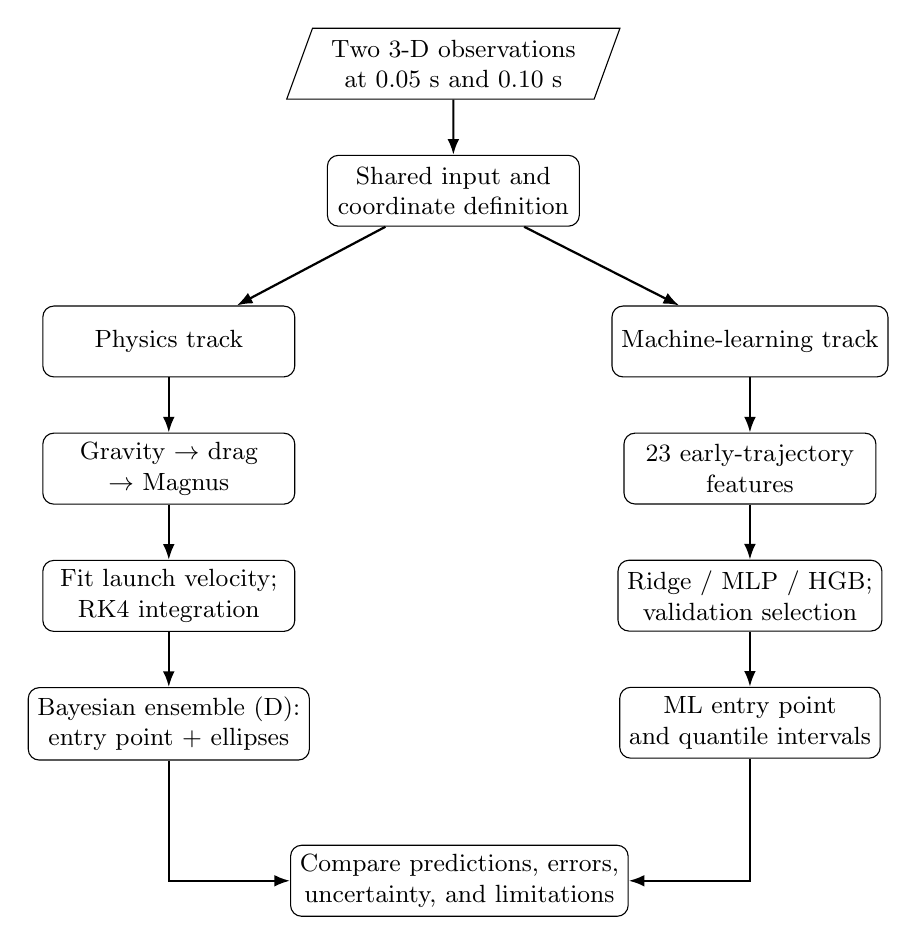
\begin{tikzpicture}[
 node distance=7mm and 9mm,
 block/.style={draw,rounded corners,align=center,minimum width=32mm,minimum height=9mm,font=\small},
 data/.style={draw, trapezium,trapezium left angle=70,trapezium right angle=110,align=center,minimum width=32mm,minimum height=9mm,font=\small},
 decision/.style={draw,diamond,aspect=2,align=center,inner sep=1pt,font=\small},
 arr/.style={-{Latex[length=2mm]},thick}
]
\node[data] (obs) {Two 3-D observations\\at 0.05 s and 0.10 s};
\node[block,below=of obs] (split) {Shared input and\\coordinate definition};
\node[block,below left=10mm and 4mm of split] (phys) {Physics track};
\node[block,below right=10mm and 4mm of split] (ml) {Machine-learning track};
\node[block,below=of phys] (layers) {Gravity $\rightarrow$ drag\\$\rightarrow$ Magnus};
\node[block,below=of layers] (ode) {Fit launch velocity;\\RK4 integration};
\node[block,below=of ml] (features) {23 early-trajectory\\features};
\node[block,below=of features] (models) {Ridge / MLP / HGB;\\validation selection};
\node[block,below=of ode] (physout) {Bayesian ensemble (D):\\entry point + ellipses};
\node[block,below=of models] (mlout) {ML entry point\\and quantile intervals};
\node[block] (compare) at ($(physout)!0.5!(mlout)+(0,-20mm)$) {Compare predictions, errors,\\uncertainty, and limitations};
\draw[arr] (obs)--(split);
\draw[arr] (split)--(phys);
\draw[arr] (split)--(ml);
\draw[arr] (phys)--(layers);
\draw[arr] (layers)--(ode);
\draw[arr] (ode)--(physout);
\draw[arr] (ml)--(features);
\draw[arr] (features)--(models);
\draw[arr] (models)--(mlout);
\draw[arr] (physout.south) |- (compare.west);
\draw[arr] (mlout.south) |- (compare.east);
\end{tikzpicture}%
}
\caption{Workflow for the physics-based and machine-learning approaches.}
\label{fig:workflow}
\end{figure}

\section{Problem Definition and Coordinate System}
The ball centre starts at
\begin{equation}
    \bm r_0=(0,0,R), \qquad R=0.11\ {\rm m},
\end{equation}
and the goal plane is
\begin{equation}
    x_{\rm goal}=11\ {\rm m}.
\end{equation}
The goal opening is represented by
\begin{equation}
    -3.66 < y < 3.66,\qquad 0<z<2.44.
\end{equation}
The observed positions are
\begin{align}
    \bm r_1 &= (1.50,\,0.45,\,0.44)\ {\rm m}, & t_1&=0.05\ {\rm s},\\
    \bm r_2 &= (2.96,\,0.86,\,0.74)\ {\rm m}, & t_2&=0.10\ {\rm s}.
\end{align}
The target is
\begin{equation}
    \bm r_{\rm goal}=(11,y_{\rm goal},z_{\rm goal}),
\end{equation}
where the trajectory is evaluated at its first crossing of $x=11$ m. The ball is treated as a point mass at its centre; its finite radius is used in the aerodynamic cross-sectional area. Figure~\ref{fig:fig1} shows the geometry: $x$ points from the penalty spot towards the goal, $y$ is the lateral coordinate and $z$ is the height above the ground.


\begin{figure*}[h!]
    \centering
    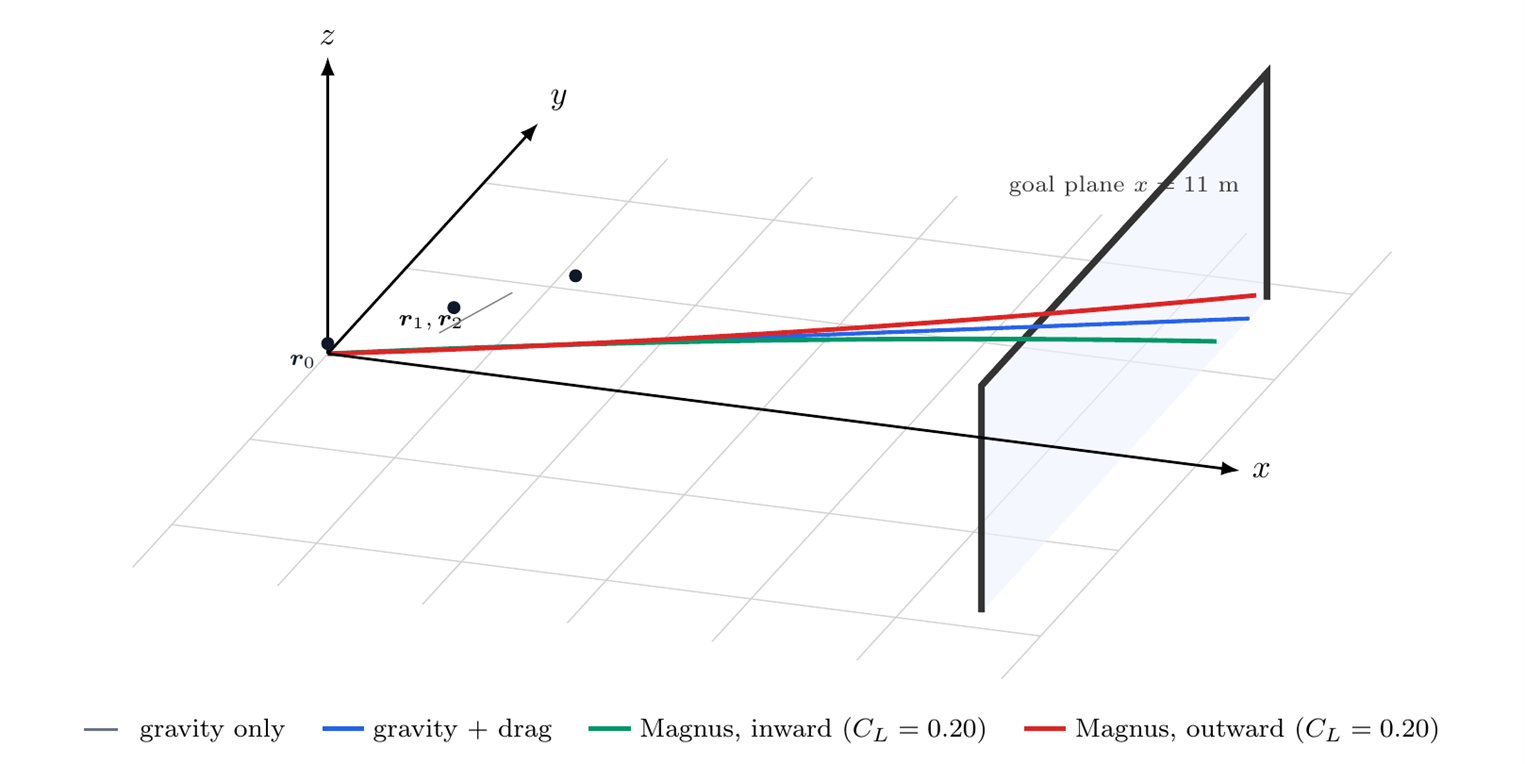
\includegraphics[width=5in]{Figure/Figure1.png}
    \caption{Geometry of the problem and fitted trajectories. Black dots are the known start r₀ and the two observations; the shaded rectangle is the goal opening at x = 11 m. The four curves are the RK4 solutions of the three model layers fitted to the same two observations.}
    \label{fig:fig1}
\end{figure*}

\section{Physical Model}

\subsection{Parameters and assumptions}
The base physical parameters are listed in Table~\ref{tab:parameters}. The derived drag and lift factors $k_D$ and $k_L$ (defined in Eq.~\eqref{eq:kdkl}) are included for reference.

\begin{table}[H]
\centering
\caption{Physical parameters used in the model.}
\label{tab:parameters}
\begin{tabular}{lll}
\toprule
Parameter & Symbol & Value\\
\midrule
Ball mass & $m$ & $0.43$ kg\\
Ball radius & $R$ & $0.11$ m\\
Cross-sectional area & $A=\pi R^2$ & $0.0380$ m$^2$\\
Air density & $\rho$ & $1.2$ kg m$^{-3}$\\
Dynamic viscosity & $\mu$ & $1.8\times10^{-5}$ Pa s\\
Gravitational acceleration & $g$ & $9.81$ m s$^{-2}$\\
Observation times & $t_1,t_2$ & $0.05,\,0.10$ s\\
Position-noise standard deviation & $\sigma$ & $0.0058$ m\\
Goal-plane coordinate & $x_{\rm goal}$ & $11$ m\\
Drag factor ($C_D=0.22$) & $k_D$ & $0.01167$ m$^{-1}$\\
Lift factor per unit $C_L$ & $k_L/C_L$ & $0.05304$ m$^{-1}$\\
\bottomrule
\end{tabular}
\end{table}

The base model assumes a rigid spherical ball, constant air density, still air, constant drag and lift coefficients over the short flight, and constant spin vector. Ground contact is excluded from the base trajectory model. Measurement noise is treated as independent Gaussian noise with standard deviation $\sigma$ in each coordinate.

\subsection{Aerodynamic parameters}
The cross-sectional area and the drag and lift factors follow the standard aerodynamic force formulation for sports balls \citep{mehta1985,asai2007}:
\begin{equation}
 A=\pi R^2,\qquad
 k_D=\frac{\rho C_D A}{2m},\qquad
 k_L=\frac{\rho C_L A}{2m}.
 \label{eq:kdkl}
\end{equation}
Both have units of m$^{-1}$, so that $k_D\|\bm v\|\bm v$ and $k_L\|\bm v\|^2$ are accelerations. The Reynolds number is
\begin{equation}
    \mathrm{Re}=\frac{\rho \|\bm v\|D}{\mu},\qquad D=2R.
\end{equation}


\paragraph{Representative speed.}
The speed can be estimated from both observation intervals. The mean velocities over $[0,t_1]$ and $[t_1,t_2]$ are
\begin{align}
    \bar{\bm v}_{01}&=\frac{\bm r_1-\bm r_0}{t_1}
    =\frac{(1.50,\,0.45,\,0.33)}{0.05}=(30.0,\;9.0,\;6.6)\ {\rm m\,s^{-1}},\\
    \bar{\bm v}_{12}&=\frac{\bm r_2-\bm r_1}{t_2-t_1}
    =\frac{(1.46,\,0.41,\,0.30)}{0.05}=(29.2,\;8.2,\;6.0)\ {\rm m\,s^{-1}},
\end{align}
with corresponding speeds
\begin{equation}
    \|\bar{\bm v}_{01}\|\approx32.0\ {\rm m\,s^{-1}},\qquad
    \|\bar{\bm v}_{12}\|\approx30.9\ {\rm m\,s^{-1}}.
\end{equation}
The mean speed over the whole window is $\|(\bm r_2-\bm r_0)/t_2\|\approx31.5$ m\,s$^{-1}$, and the fitted launch speed is $\|\widehat{\bm v}_0\|\approx32.2$ m\,s$^{-1}$. The speed falls by about $1$ m\,s$^{-1}$ between the two intervals, which is the same order as the deceleration predicted by the model, $(k_D\|\bm v\|^2+g\,\hat v_z)\,\Delta t\approx0.7$ m\,s$^{-1}$, with $\Delta t=0.05$ s between the interval midpoints. The corresponding Reynolds numbers are
\begin{equation}
    \mathrm{Re}=\frac{\rho\|\bm v\|D}{\mu}:\qquad
    \frac{1.2\times32.0\times0.22}{1.8\times10^{-5}}\approx4.7\times10^{5},\qquad
    \frac{1.2\times30.9\times0.22}{1.8\times10^{-5}}\approx4.5\times10^{5}.
\end{equation}
Both values lie in the same supercritical regime, so $v=32$ m\,s$^{-1}$ is used as the representative speed and $C_D\in[0.20,0.25]$ is retained. Inside the model, $\|\bm v\|$ is recomputed at every RK4 step. Within this range $C_D=0.22$ is used as the central setting. The lift coefficient is varied over $C_L\in[0.10,0.25]$ in accordance with trajectory and curve-kick studies \citep{goff2010,carre2002} for the illustrative sidespin cases. These ranges are modelling priors rather than quantities identified uniquely by the two observations. Figure~\ref{fig:fig2} compares the size of the three accelerations at the fitted launch speed $\|\bm v_0\|\approx32.0$ m s$^{-1}$: drag and Magnus acceleration are both of the same order as gravity, so none of them can be neglected a priori.



\begin{figure*}[h!]
    \centering
    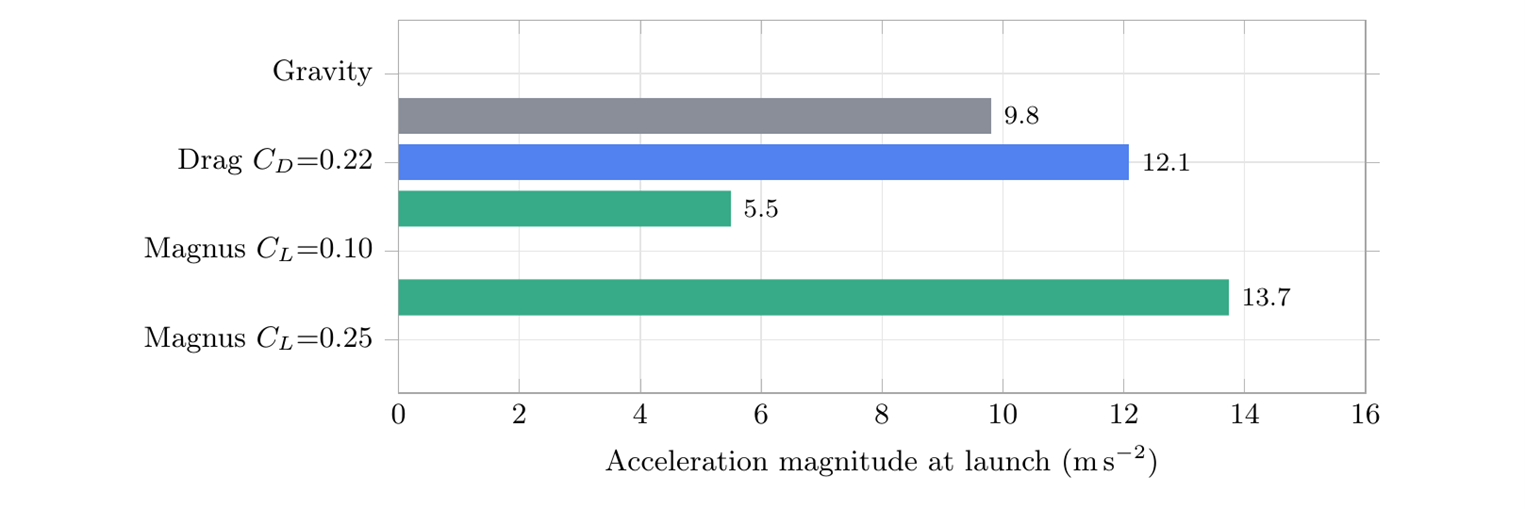
\includegraphics[width=5in]{Figure/Figure2.png}
    \caption{Acceleration budget at the fitted launch speed}
    \label{fig:fig2}
\end{figure*}


\subsection{Layer 1: gravity-only trajectory}
The simplest model is
\begin{equation}
    \frac{d\bm r}{dt}=\bm v,\qquad
    \frac{d\bm v}{dt}=\bm g,\qquad
    \bm g=(0,0,-g).
\end{equation}
Its closed-form position is
\begin{equation}
    \bm r(t)=\bm r_0+\bm v_0t+\frac{1}{2}\bm g t^2.
\end{equation}
For each observation define
\begin{equation}
    \bm d_i=\bm r_i-\bm r_0-\frac{1}{2}\bm g t_i^2.
\end{equation}
Minimising $\sum_i\|\bm d_i-\bm v_0t_i\|^2$ over $\bm v_0$ (set the gradient to zero) gives the least-squares estimate of the initial velocity,
\paragraph{Derivation of $\widehat{\bm v}_0$.}
Minimizing $S(\bm v_0)=\sum_{i=1}^{2}\|\bm d_i-\bm v_0t_i\|^2$ and setting $\partial S/\partial\bm v_0=-2\sum_i t_i(\bm d_i-\bm v_0t_i)=\bm 0$ gives
$\widehat{\bm v}_0=\sum_i t_i\bm d_i\big/\sum_i t_i^2$, which is the expression above.

\paragraph{Numerical evaluation.}
The gravity terms are
\begin{equation}
    \tfrac12 g t_1^2=\tfrac12(9.81)(0.05)^2=0.0122625\ {\rm m},\qquad
    \tfrac12 g t_2^2=\tfrac12(9.81)(0.10)^2=0.04905\ {\rm m},
\end{equation}
and since $\bm g=(0,0,-g)$ they affect only the $z$ component. With $\bm r_0=(0,0,0.11)$,
\begin{align}
    \bm d_1&=\bm r_1-\bm r_0-\tfrac12\bm g t_1^2
    =(1.50,\;0.45,\;0.44-0.11+0.0122625)=(1.50,\;0.45,\;0.3422625)\ {\rm m},\\
    \bm d_2&=\bm r_2-\bm r_0-\tfrac12\bm g t_2^2
    =(2.96,\;0.86,\;0.74-0.11+0.04905)=(2.96,\;0.86,\;0.67905)\ {\rm m}.
\end{align}
The weighted sum and the denominator are
\begin{align}
    t_1\bm d_1&=0.05\,\bm d_1=(0.0750,\;0.0225,\;0.0171131)\ {\rm m\,s},\\
    t_2\bm d_2&=0.10\,\bm d_2=(0.2960,\;0.0860,\;0.0679050)\ {\rm m\,s},\\
    t_1\bm d_1+t_2\bm d_2&=(0.3710,\;0.1085,\;0.0850181)\ {\rm m\,s},\\
    t_1^2+t_2^2&=0.0025+0.0100=0.0125\ {\rm s^2}.
\end{align}
Therefore
\begin{equation}
    \widehat{\bm v}_0=\frac{(0.3710,\;0.1085,\;0.0850181)}{0.0125}
    =(29.68,\;8.68,\;6.80)\ {\rm m\,s^{-1}}.
\end{equation}

\paragraph{Goal-plane crossing.}
Because there is no drag in this layer, $v_x$ is constant and $x(t)=\widehat v_{0x}t$. The plane $x=11$ m is reached at
\begin{equation}
    T=\frac{x_{\rm goal}}{\widehat v_{0x}}=\frac{11}{29.68}=0.3706\ {\rm s}\approx0.371\ {\rm s}.
\end{equation}
Substituting $T$ into the ballistic equation $\bm r(t)=\bm r_0+\widehat{\bm v}_0t+\tfrac12\bm g t^2$:
\begin{align}
    y_{\rm goal}&=0+\widehat v_{0y}\,T=8.68\times0.3706=3.217\ {\rm m}\approx3.22\ {\rm m},\\
    z_{\rm goal}&=R+\widehat v_{0z}\,T-\tfrac12 gT^2\notag\\
    &=0.11+6.80145\times0.3706-\tfrac12(9.81)(0.3706)^2\notag\\
    &=0.11+2.5208-0.6737=1.957\ {\rm m}\approx1.96\ {\rm m}.
\end{align}
Hence $(x,y,z)_{\rm goal}=(11,\;3.22,\;1.96)$ m for the gravity-only layer.


\subsection{Layer 2: gravity and quadratic drag}
Quadratic drag acts opposite to the velocity:
\begin{equation}
    \frac{d\bm v}{dt}
    =\bm g-k_D\|\bm v\|\bm v
    =\bm g-\frac{\rho C_D A}{2m}\|\bm v\|\bm v.
    \label{eq:drag}
\end{equation}

\paragraph{Drag factor.}
With $A=\pi R^2=\pi(0.11)^2=0.038013$ m$^2$,
\begin{equation}
    k_D=\frac{\rho C_D A}{2m}=\frac{1.2\times C_D\times0.038013}{2\times0.43}
    =0.05304\,C_D\ {\rm m^{-1}}.
\end{equation}
Hence
\begin{equation}
    k_D(C_D{=}0.20)=0.01061,\qquad
    k_D(C_D{=}0.22)=0.01167,\qquad
    k_D(C_D{=}0.25)=0.01326\ \ {\rm m^{-1}}.
\end{equation}

\paragraph{Component form.}
Writing $v=\|\bm v\|=\sqrt{v_x^2+v_y^2+v_z^2}$,
\begin{equation}
    \dot v_x=-k_D v\,v_x,\qquad
    \dot v_y=-k_D v\,v_y,\qquad
    \dot v_z=-g-k_D v\,v_z .
\end{equation}
Equation~\eqref{eq:drag} has no closed-form solution, because $v$ couples the three components, so it is integrated with RK4.

\paragraph{Drag does not change the lateral direction.}
Let $u=v_y/v_x$. Then
\begin{equation}
    \dot u=\frac{\dot v_y v_x-v_y\dot v_x}{v_x^2}
    =\frac{(-k_Dv\,v_y)v_x-v_y(-k_Dv\,v_x)}{v_x^2}=0 .
\end{equation}
So $v_y/v_x=v_{0y}/v_{0x}$ for all $t$, and the path in the $x$--$y$ plane is a straight line:
\begin{equation}
    y(t)=\frac{v_{0y}}{v_{0x}}\,x(t)
    \quad\Rightarrow\quad
    y_{\rm goal}=x_{\rm goal}\frac{v_{0y}}{v_{0x}}=11\times\frac{8.826}{30.178}=3.22\ {\rm m}.
\end{equation}
This is the same value as in Layer~1, where $11\times8.68/29.68=3.22$ m, because the two fits give the same ratio $v_{0y}/v_{0x}\approx0.2925$.

\paragraph{Size of the drag effect at launch.}
For the fitted launch velocity $\bm v_0=(30.18,\,8.83,\,6.91)$ m\,s$^{-1}$ (Table~\ref{tab:layer2_fit}) $\|\bm v_0\|=\sqrt{30.18^2+8.83^2+6.91^2}=32.19$ m\,s$^{-1}$, and the initial acceleration is
\begin{align}
    a_x&=-k_D v\,v_x=-0.01167\times32.19\times30.18=-11.34\ {\rm m\,s^{-2}},\\
    a_y&=-k_D v\,v_y=-0.01167\times32.19\times8.83=-3.32\ {\rm m\,s^{-2}},\\
    a_z&=-g-k_D v\,v_z=-9.81-0.01167\times32.19\times6.91=-12.41\ {\rm m\,s^{-2}}.
\end{align}
The rate of change of speed is
\begin{equation}
    \dot v=\hat{\bm v}\cdot\bm a=-k_Dv^2-g\,\hat v_z
    =-0.01167\,(32.19)^2-9.81\times\frac{6.91}{32.19}
    =-12.09-2.11=-14.2\ {\rm m\,s^{-2}},
\end{equation}
so the ball loses about $0.7$ m\,s$^{-1}$ in $0.05$ s.

\paragraph{Analytic estimate of the flight time.}
If the direction of motion is approximated as fixed (neglecting the bending by gravity), $\dot v=-k_Dv^2$ gives $v=v_0e^{-k_Ds}$ along the path length $s$, and $v_x=v_{0x}e^{-k_Ds}$ with $s=x/\cos\varphi$, $\cos\varphi=v_{0x}/\|\bm v_0\|=0.9376$. Define $k'=k_D/\cos\varphi=0.01245$ m$^{-1}$. Then $dx/dt=v_{0x}e^{-k'x}$ integrates to
\begin{equation}
    T\approx\frac{e^{k'x_{\rm goal}}-1}{k'v_{0x}}
    =\frac{e^{0.1369}-1}{0.01245\times30.18}=\frac{0.1467}{0.3756}=0.391\ {\rm s},
\end{equation}
in agreement with the RK4 value $T=0.390$ s. The flight time is longer than the gravity-only value $0.371$ s because the horizontal speed drops from $30.2$ m\,s$^{-1}$ to roughly $26$ m\,s$^{-1}$ at the goal plane; the extra $0.019$ s increases the gravitational drop.

\paragraph{Fitted results.}
For each $C_D$ the three components of $\bm v_0$ were fitted by minimising Eq.~\eqref{eq:fit}, and the goal-plane values were obtained with RK4 ($\Delta t=10^{-3}$ s):
\begin{table}[H]
\centering
\small
\caption{Layer-2 fits for three drag coefficients (gravity and quadratic drag): fitted launch velocity, flight time, entry height and residual statistic.}
\label{tab:layer2_fit}
\begin{tabular}{rrrrrrr}
\toprule
$C_D$ & $v_{0x}$ & $v_{0y}$ & $v_{0z}$ & $T$ (s) & $z_{\rm goal}$ (m) & $\chi^2$\\
\midrule
0.20 & 30.13 & 8.81 & 6.90 & 0.389 & 1.92 & 7.76\\
0.22 & 30.18 & 8.83 & 6.91 & 0.390 & 1.91 & 7.07\\
0.25 & 30.25 & 8.85 & 6.93 & 0.393 & 1.91 & 6.19\\
\bottomrule
\end{tabular}
\end{table}

In all cases $y_{\rm goal}=3.22$ m. Compared with Layer~1, drag raises the flight time by $0.018$--$0.022$ s and lowers the entry height from $1.96$ m to $1.91$--$1.92$ m. The residual $\chi^2=6.2$--$7.8$ for six measurements and three fitted parameters ($p\approx0.05$--$0.10$) is only marginal on its own; the stronger evidence is the $2.4\sigma$ lateral acceleration discussed in Section~\ref{sec:fdsec}. Together they indicate that a purely planar-straight lateral path does not fully explain the observed lateral curvature; this motivates Layer~3.



\subsection{Layer 3: gravity, drag, and Magnus force}
Spin produces a Magnus force perpendicular to both the spin axis and the velocity \citep{carre2002,goff2010}. Let $\hat{\bm s}$ be the unit spin-axis vector and $\hat{\bm v}=\bm v/\|\bm v\|$. The acceleration model is
\begin{equation}
    \frac{d\bm v}{dt}
    =\bm g-k_D\|\bm v\|\bm v
    +k_L\|\bm v\|^2(\hat{\bm s}\times\hat{\bm v}).
    \label{eq:magnus}
\end{equation}
Equivalently, the Magnus term can be written as
\begin{equation}
    \bm a_M=\frac{\rho C_L A}{2m}\|\bm v\|^2
    (\hat{\bm s}\times\hat{\bm v}).
\end{equation}
The sign and direction of $\hat{\bm s}$ determine the direction of the lateral bend. This term is central to the uncertainty in $y_{\rm goal}$.

\begin{figure*}[h!]
    \centering
    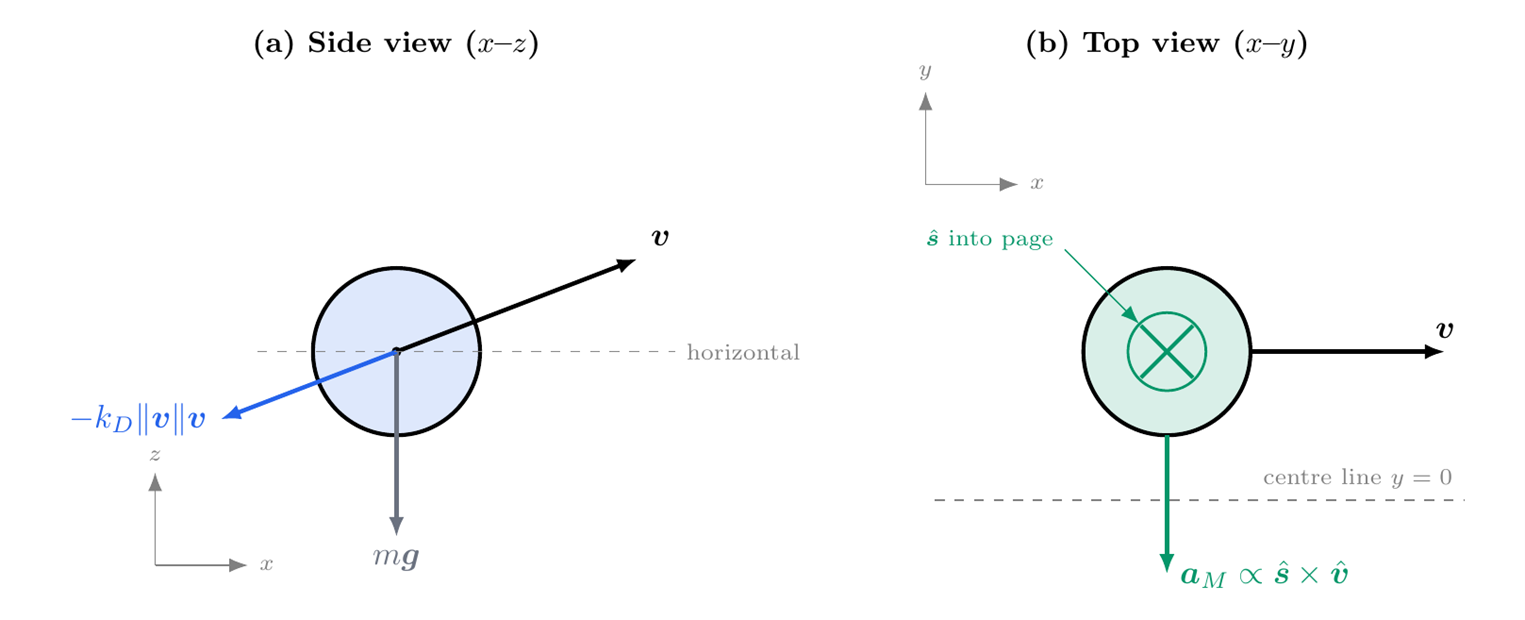
\includegraphics[width=5in]{Figure/Figure3.png}
    \caption{Force decomposition. (a) Gravity and quadratic drag lie in the plane of motion. (b) For sidespin with $\hat{\bm s}=-\hat{\bm z}$ (axis into the page in the top view), $\hat{\bm s}\times\hat{\bm v}$ points towards $-y$, i.e.\ the ball curves towards the centre line.}
    \label{fig:fig3}
\end{figure*}





For a pure sidespin about the vertical axis, $\hat{\bm s}=\mp\hat{\bm z}$, the cross product gives $\hat{\bm s}\times\hat{\bm v}=\mp(-\hat v_y,\hat v_x,0)$, so the lateral acceleration is
\begin{equation}
    a_y=-\|\bm v\|\bigl(k_D v_y+k_L v_x\bigr)\quad(\hat{\bm s}=-\hat{\bm z},\ \text{inward}).
    \label{eq:ay}
\end{equation}
Here $\hat{\bm s}=-\hat{\bm z}$ is the ``inward'' case, in which the ball curves towards the centre line $y=0$; $\hat{\bm s}=+\hat{\bm z}$ reverses the sign of the $k_L$ term (``outward''). Figure~\ref{fig:fig3} illustrates the forces and the direction of the Magnus term.

\textbf{Model Hierarchy:} 
The three layers are nested: each adds exactly one physical effect to the
previous one (Figure~\ref{fig:fig4}):

\begin{figure*}[h!]
    \centering
    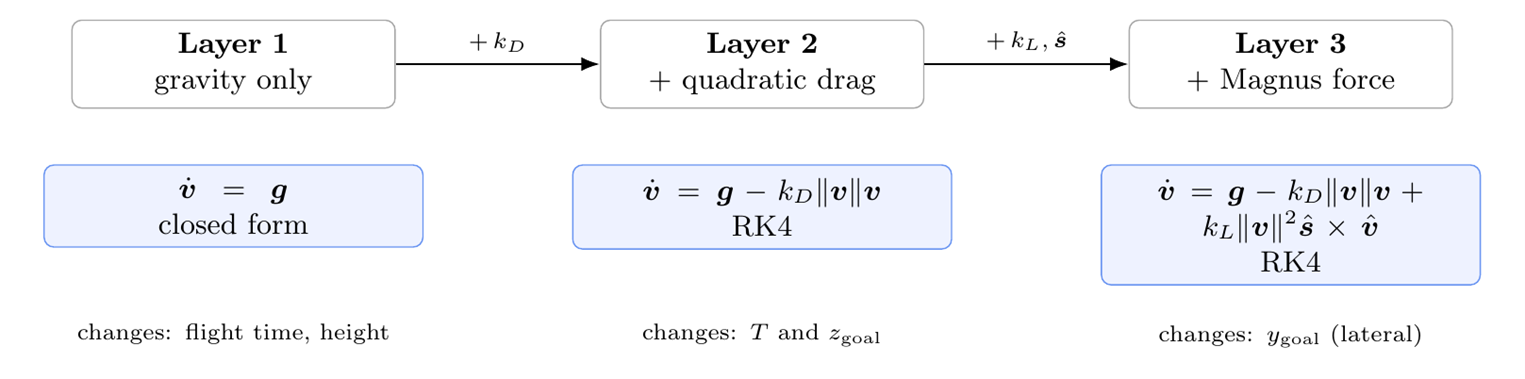
\includegraphics[width=\linewidth]{hellofig.png}
    \caption{Nested model layers and the dominant effect of each added term.}
    \label{fig:fig4}
\end{figure*}



\subsection{Numerical integration and parameter fitting}
The state vector is $\bm q=(\bm r,\bm v)$. The classical fourth-order Runge--Kutta scheme is used for numerical integration \citep{press2007}. Equations~\eqref{eq:drag}--\eqref{eq:magnus} are integrated using classical fourth-order Runge--Kutta (RK4) with step size
\begin{equation}
    \Delta t=10^{-3}\ {\rm s}.
\end{equation}
With $\bm q'=\bm f(\bm q)$, one step is
\begin{equation}
\begin{aligned}
 \bm k_1&=\bm f(\bm q_n), & \bm k_2&=\bm f\!\left(\bm q_n+\tfrac{\Delta t}{2}\bm k_1\right),\\
 \bm k_3&=\bm f\!\left(\bm q_n+\tfrac{\Delta t}{2}\bm k_2\right), & \bm k_4&=\bm f(\bm q_n+\Delta t\,\bm k_3),\\
 \bm q_{n+1}&=\bm q_n+\tfrac{\Delta t}{6}(\bm k_1+2\bm k_2+2\bm k_3+\bm k_4).
\end{aligned}
\end{equation}
The crossing of $x=11$ m is linearly interpolated between the last point before and the first point after the plane. For fixed aerodynamic parameters, the three components of $\bm v_0$ are fitted by nonlinear least squares:
\begin{equation}
 \widehat{\bm v}_0=
 \arg\min_{\bm v_0}
 \sum_{i=1}^{2}
 \frac{\|\bm r_{\rm model}(t_i;\bm v_0)-\bm r_i\|_2^2}{\sigma^2}.
 \label{eq:fit}
\end{equation}
The corresponding weighted residual statistic is
\begin{equation}
    \chi^2=\sum_{i=1}^{2}\sum_{j\in\{x,y,z\}}
    \left(\frac{r_{{\rm model},ij}-r_{ij}}{\sigma}\right)^2.
\end{equation}



\begin{figure*}[h!]
    \centering
    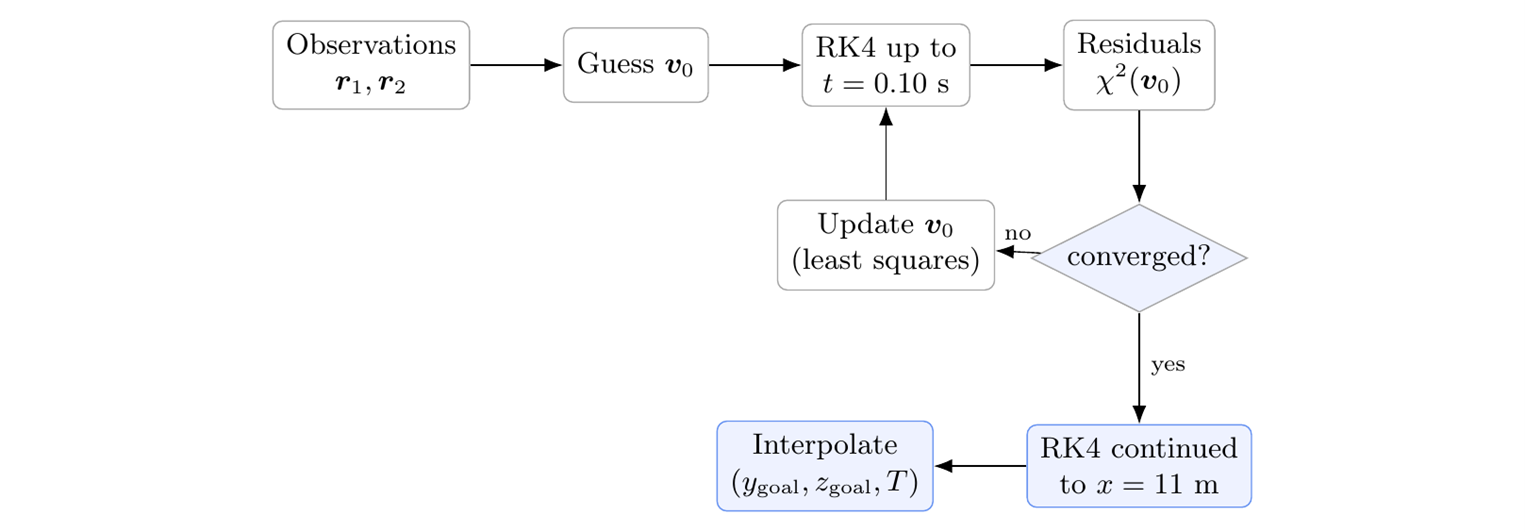
\includegraphics[width=5in]{Figure/Figure5.png}
    \caption{Inverse procedure: the launch velocity is fitted to the two observations, then the
trajectory is continued to the goal plane.}
    \label{fig:fig5}
\end{figure*}

Figure ~\ref{fig:fig5} summarizes the inner (fit) and outer (prediction) loops.

\subsection{Identifiability}
The complete aerodynamic model has three launch-velocity parameters, one drag coefficient, one spin magnitude, and two parameters describing the spin-axis direction: seven unknowns in total. The two observed 3-D positions provide six scalar measurements. Thus, the inverse problem is underdetermined without prior information or additional observations (Figure~\ref{fig:fig6}). In particular, different spin configurations can fit the early observations similarly while producing different lateral goal-plane positions. This is why the physical model is evaluated over plausible aerodynamic settings rather than claiming a unique spin estimate.

\begin{figure*}[h!]
    \centering
    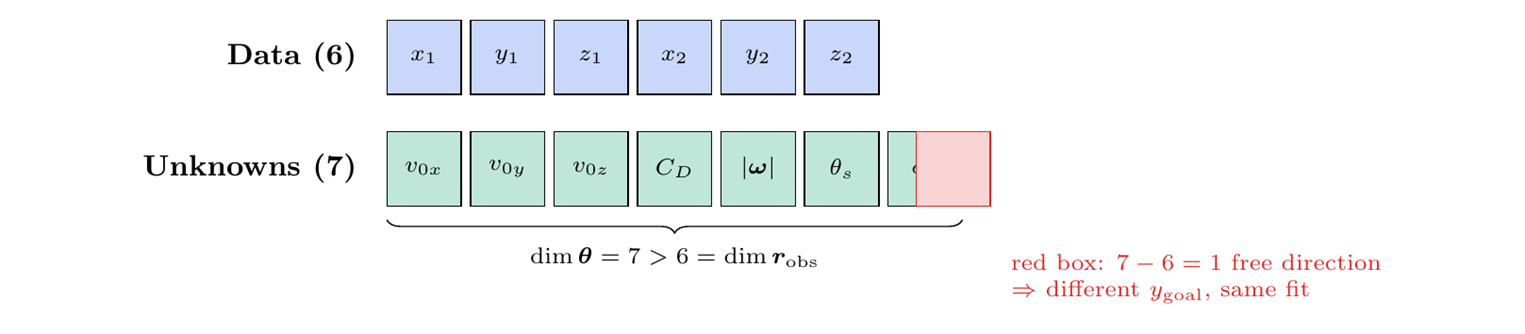
\includegraphics[width=5in]{Figure/Figure6.png}
    \caption{Parameter count: six scalar measurements cannot fix seven unknowns.}
    \label{fig:fig6}
\end{figure*}

\section{Numerical Results of the Physical Model}
The fits reproduce the following results for the supplied scenario (RK4, $\Delta t=10^{-3}$ s, $C_D=0.22$ for the Magnus layers).

\begin{table}[H]
\centering
\caption{Physical-layer results for the supplied two-observation scenario (outward spin tested at $C_L=0.10$, 0.20 and 0.25).}
\label{tab:physics}
\small
\begin{tabular}{llrrrr}
\toprule
Layer & Setting & $T$ (s) & $y_{\rm goal}$ (m) & $z_{\rm goal}$ (m) & $\chi^2$\\
\midrule
Gravity only & -- & 0.371 & 3.22 & 1.96 & --\\
Drag & $C_D=0.20$ & 0.389 & 3.22 & 1.92 & 7.76\\
Drag & $C_D=0.22$ & 0.390 & 3.22 & 1.91 & 7.07\\
Drag & $C_D=0.25$ & 0.393 & 3.22 & 1.91 & 6.19\\
Magnus, inward & $C_L=0.10$ & 0.388 & 2.94 & 1.91 & 3.9\\
Magnus, inward & $C_L=0.15$ & 0.387 & 2.81 & 1.90 & 3.0\\
Magnus, inward & $C_L=0.20$ & 0.386 & 2.67 & 1.90 & 2.7\\
Magnus, inward & $C_L=0.25$ & 0.385 & 2.54 & 1.90 & 2.8\\
Magnus, outward & $C_L=0.10$ & 0.394 & 3.50 & 1.92 & 12.2\\
Magnus, outward & $C_L=0.20$ & 0.397 & 3.80 & 1.93 & 19.3\\
Magnus, outward & $C_L=0.25$ & 0.399 & 3.95 & 1.93 & 23.6\\
\bottomrule
\end{tabular}
\end{table}

\subsection{Trajectories}
A trajectory plot such as Figure~\ref{fig:fig7} shows which physical effect controls which coordinate: gravity and drag determine height and flight time, and spin determines the lateral deviation. It also makes the identifiability problem visible. The models agree with the data at the start but diverge afterwards, so the early observations alone cannot tell which curve is correct.
\begin{figure*}[h!]
    \centering
    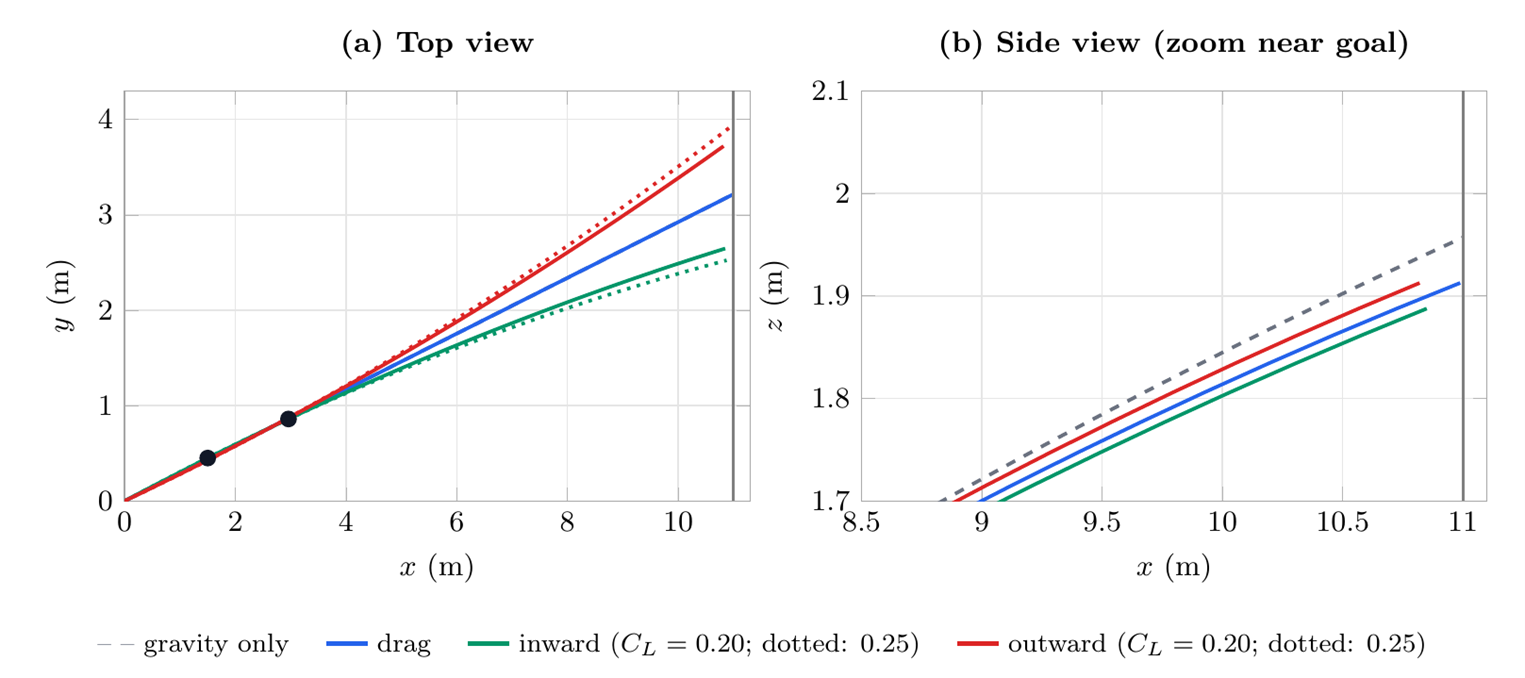
\includegraphics[width=5in]{Figure/Figure7.png}
    \caption{Fitted trajectories. (a) The lateral curvature separates the Magnus cases by more
than 1 m at the goal plane. (b) The height differs by only a few centimetres across all layers.
Black dots: observations.}
    \label{fig:fig7}
\end{figure*}

\subsection{Goal-plane entry points and Sensitivity to spin and the $\chi^2$ profile}
Scanning the signed lift coefficient $C_L$ (positive: inward, negative: outward) at $C_D=0.22$ shows \emph{what} the model predicts for $y_{\rm goal}$ and how well each spin setting fits the data ($\chi^2$), in order to test \emph{why} the lateral entry point is uncertain: $\chi^2$ is shallow in $C_L$ while $y_{\rm goal}$ changes strongly (Figures~\ref{fig:fig8} and~\ref{fig:fig9}).

\begin{figure*}[h!]
    \centering
    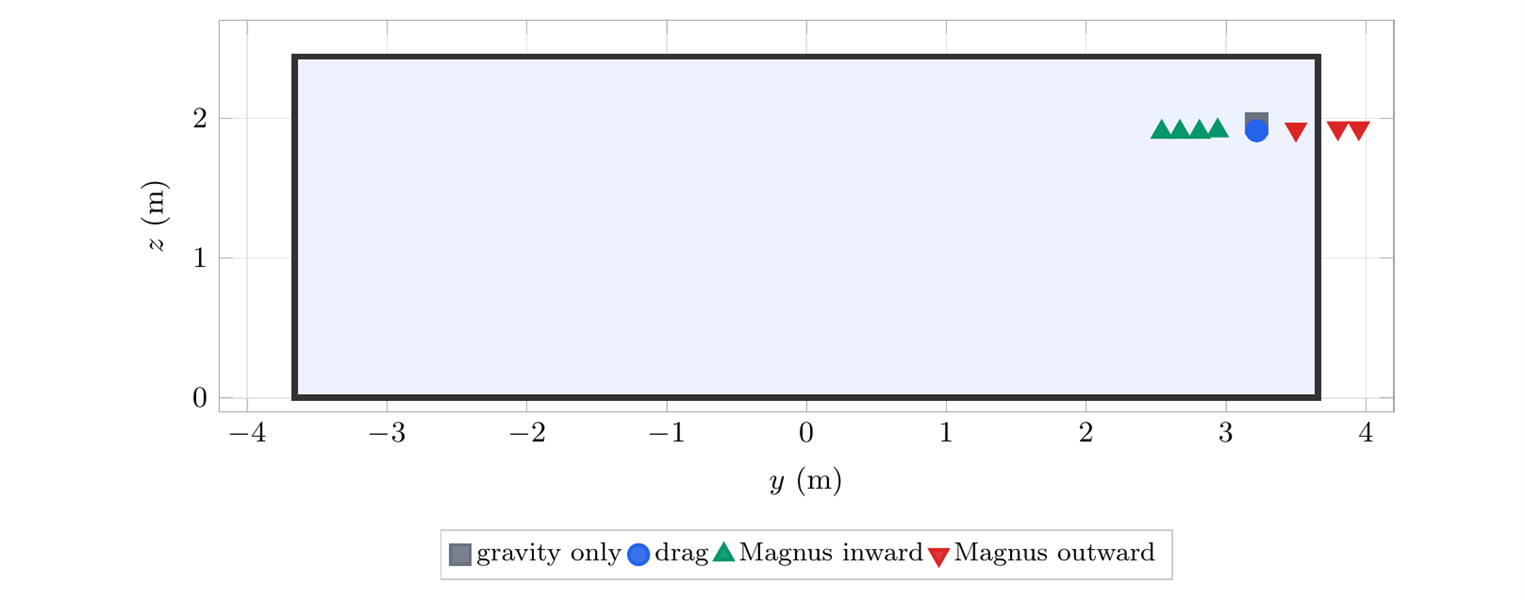
\includegraphics[width=5in]{Figure/Figure8.png}
    \caption{Predicted entry points in the goal plane as seen from the penalty spot. The shaded
rectangle is the goal opening; the outermost outward-spin point (y = 3.95 m) lies outside the
post (|y| = 3.66 m).}
    \label{fig:fig8}
\end{figure*}



\begin{figure*}[h!]
    \centering
    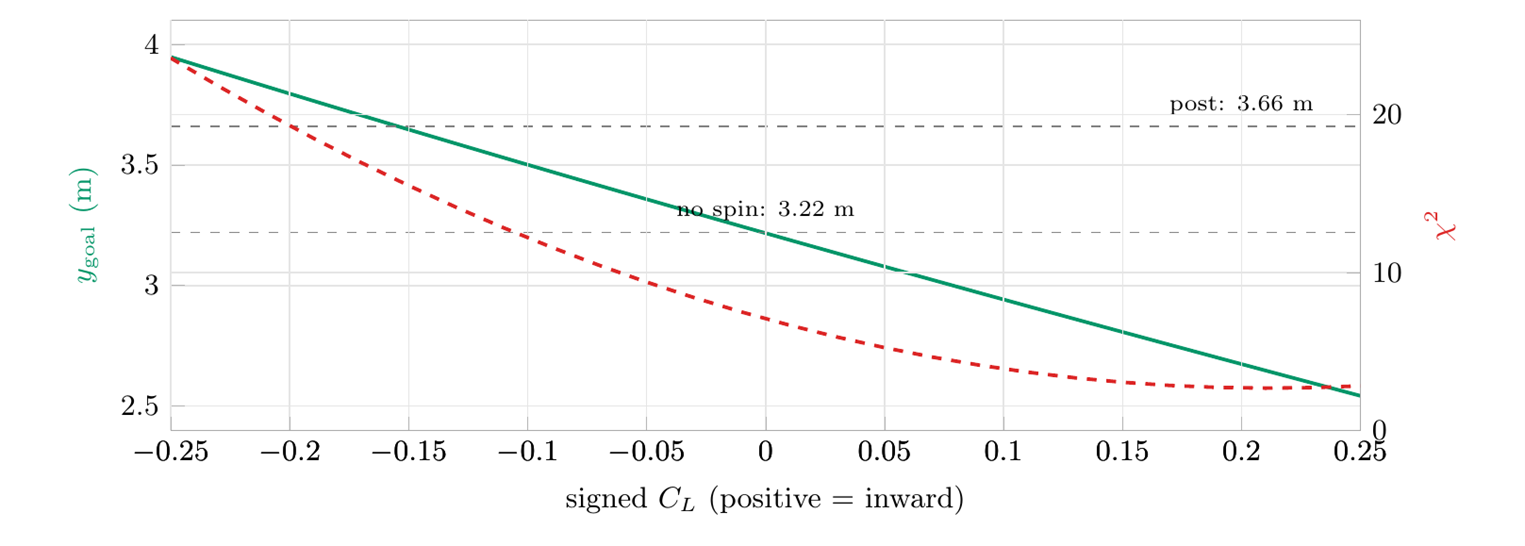
\includegraphics[width=5in]{Figure/Figure9.png}
    \caption{Lateral entry point (green, left axis) and fit quality $\chi^2$ (red dashed, right axis) versus signed $C_L$. The $\chi^2$ minimum lies near $C_L\approx0.20$--$0.25$ inward, but its shallow shape means the data cannot identify a single value, while $y_{\rm goal}$ changes by about 0.4 m over that same range.}
    \label{fig:fig9}
\end{figure*}


\subsection{Why the early data cannot fix the lateral coordinate}
\label{sec:fdsec}
Because $\bm r_0$ is known, the two observations determine a constant-acceleration model $\bm r_i=\bm r_0+\bm v_0t_i+\tfrac12\bm a t_i^2$ exactly:
\begin{equation}
    \bm a_{\rm fd}=\frac{\bm r_2-2\bm r_1+\bm r_0}{t_1t_2/2}
    =\frac{\bm r_2-2\bm r_1+\bm r_0}{0.0025\ {\rm s^2}}
    =(-16,\,-16,\,-12)\ {\rm m\,s^{-2}},
\end{equation}
with per-component standard deviation $\sigma\sqrt{1+4}/0.0025=5.2$ m s$^{-2}$ (noise on $\bm r_1,\bm r_2$ only). The model prediction at launch (Eq.~\eqref{eq:drag}, \eqref{eq:ay}) is compared with this estimate in Table~\ref{tab:fd}.


\begin{figure*}[h!]
    \centering
    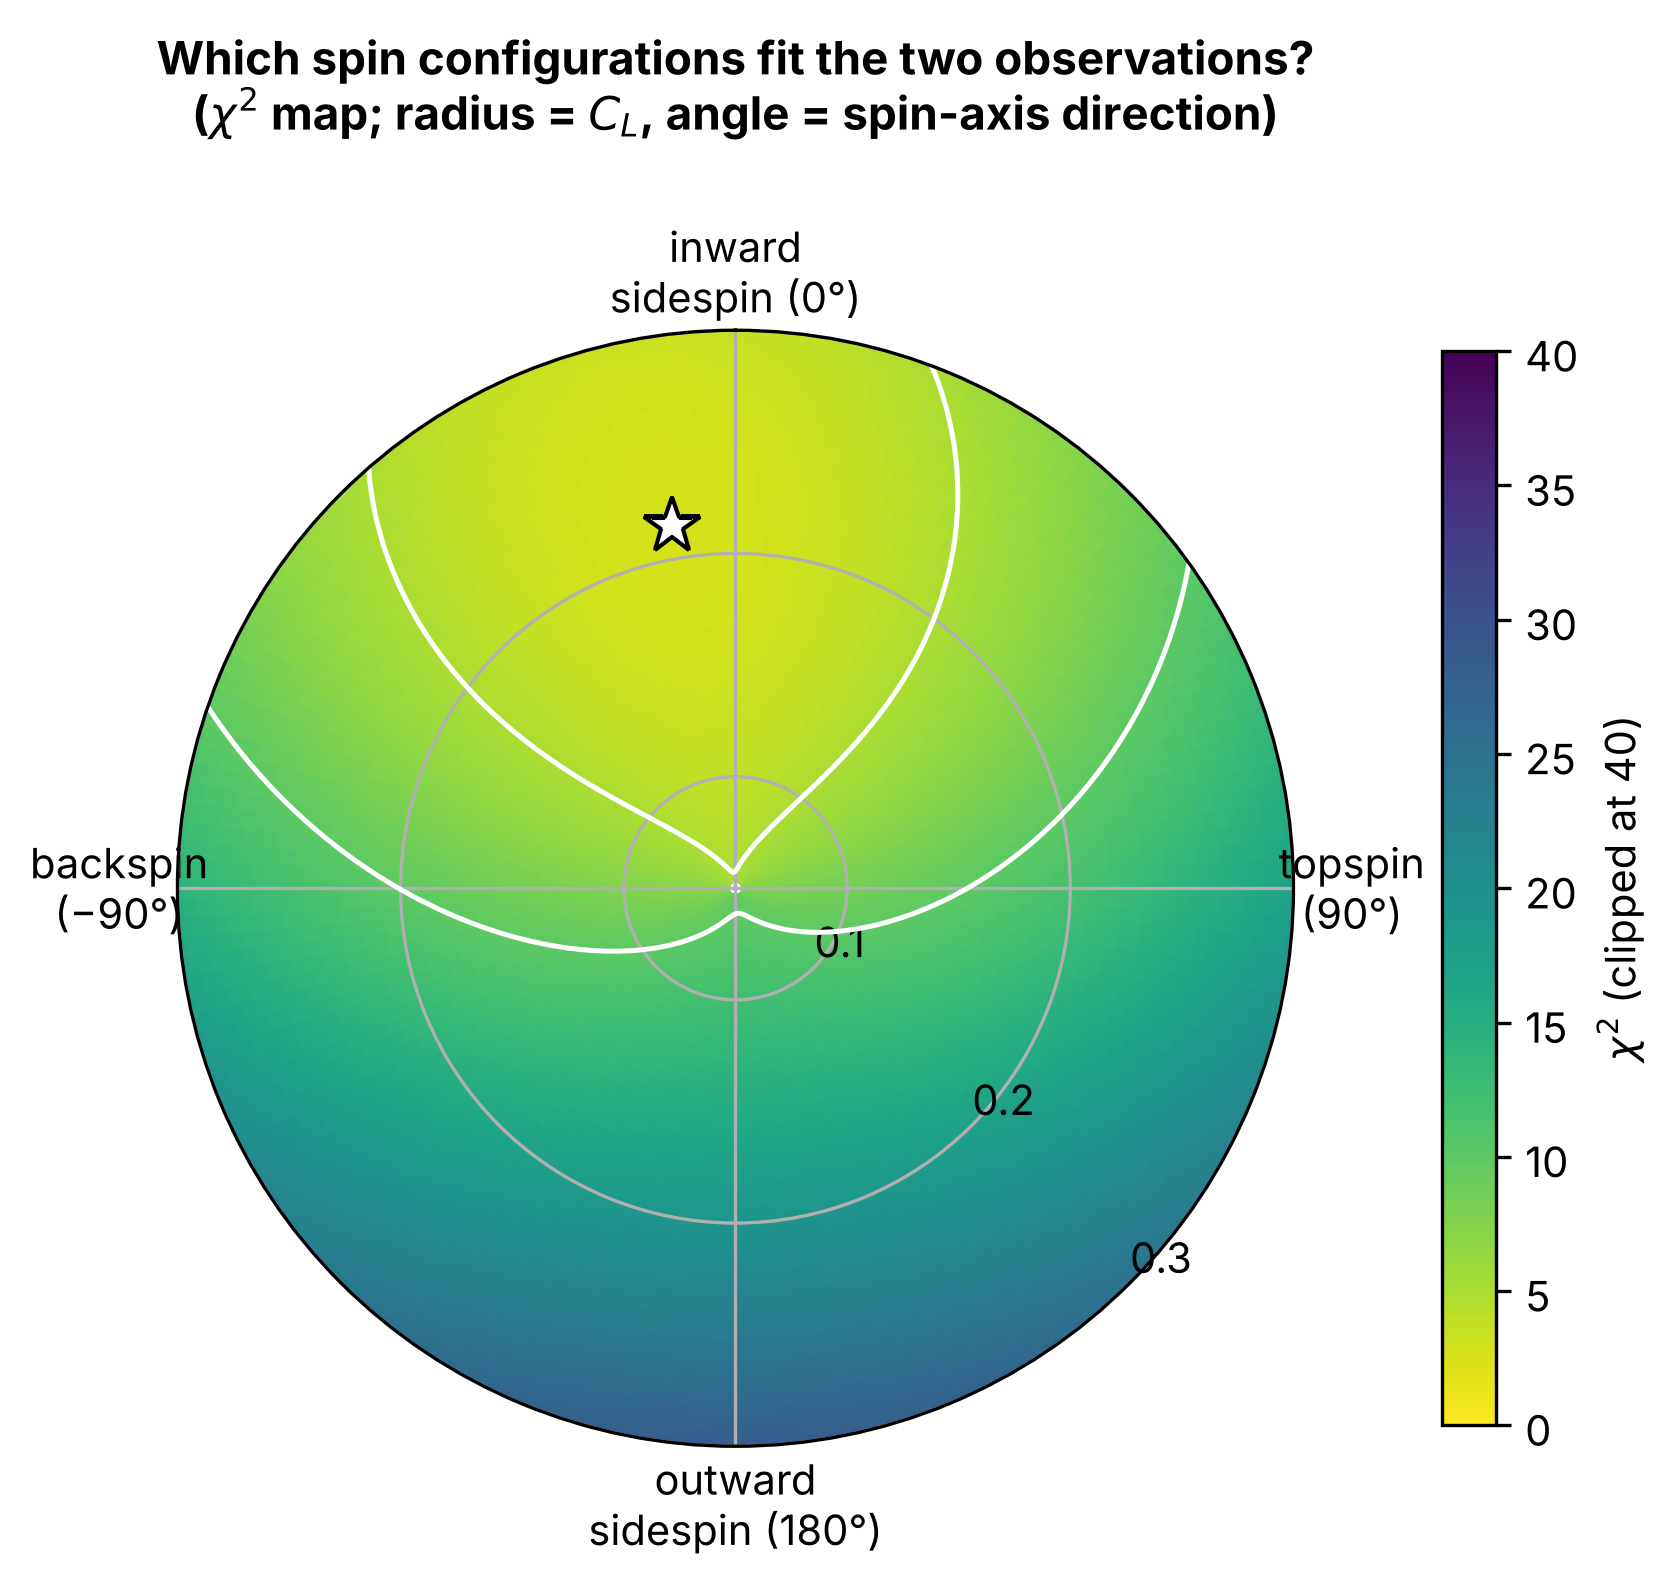
\includegraphics[width=4in]{Figure/Heat_chi2_polar.png}
    \caption{Chi-square landscape over the spin-configuration space. 
    The radial coordinate represents the lift coefficient $C_L$, 
    while the angular coordinate represents the spin-axis direction. 
    Lower $\chi^2$ values indicate better agreement with the two 
    observed positions (uniform spin-axis prior, $C_D=0.22$).}
    \label{fig:chi2polar}
\end{figure*}



\begin{figure*}[h!]
    \centering
    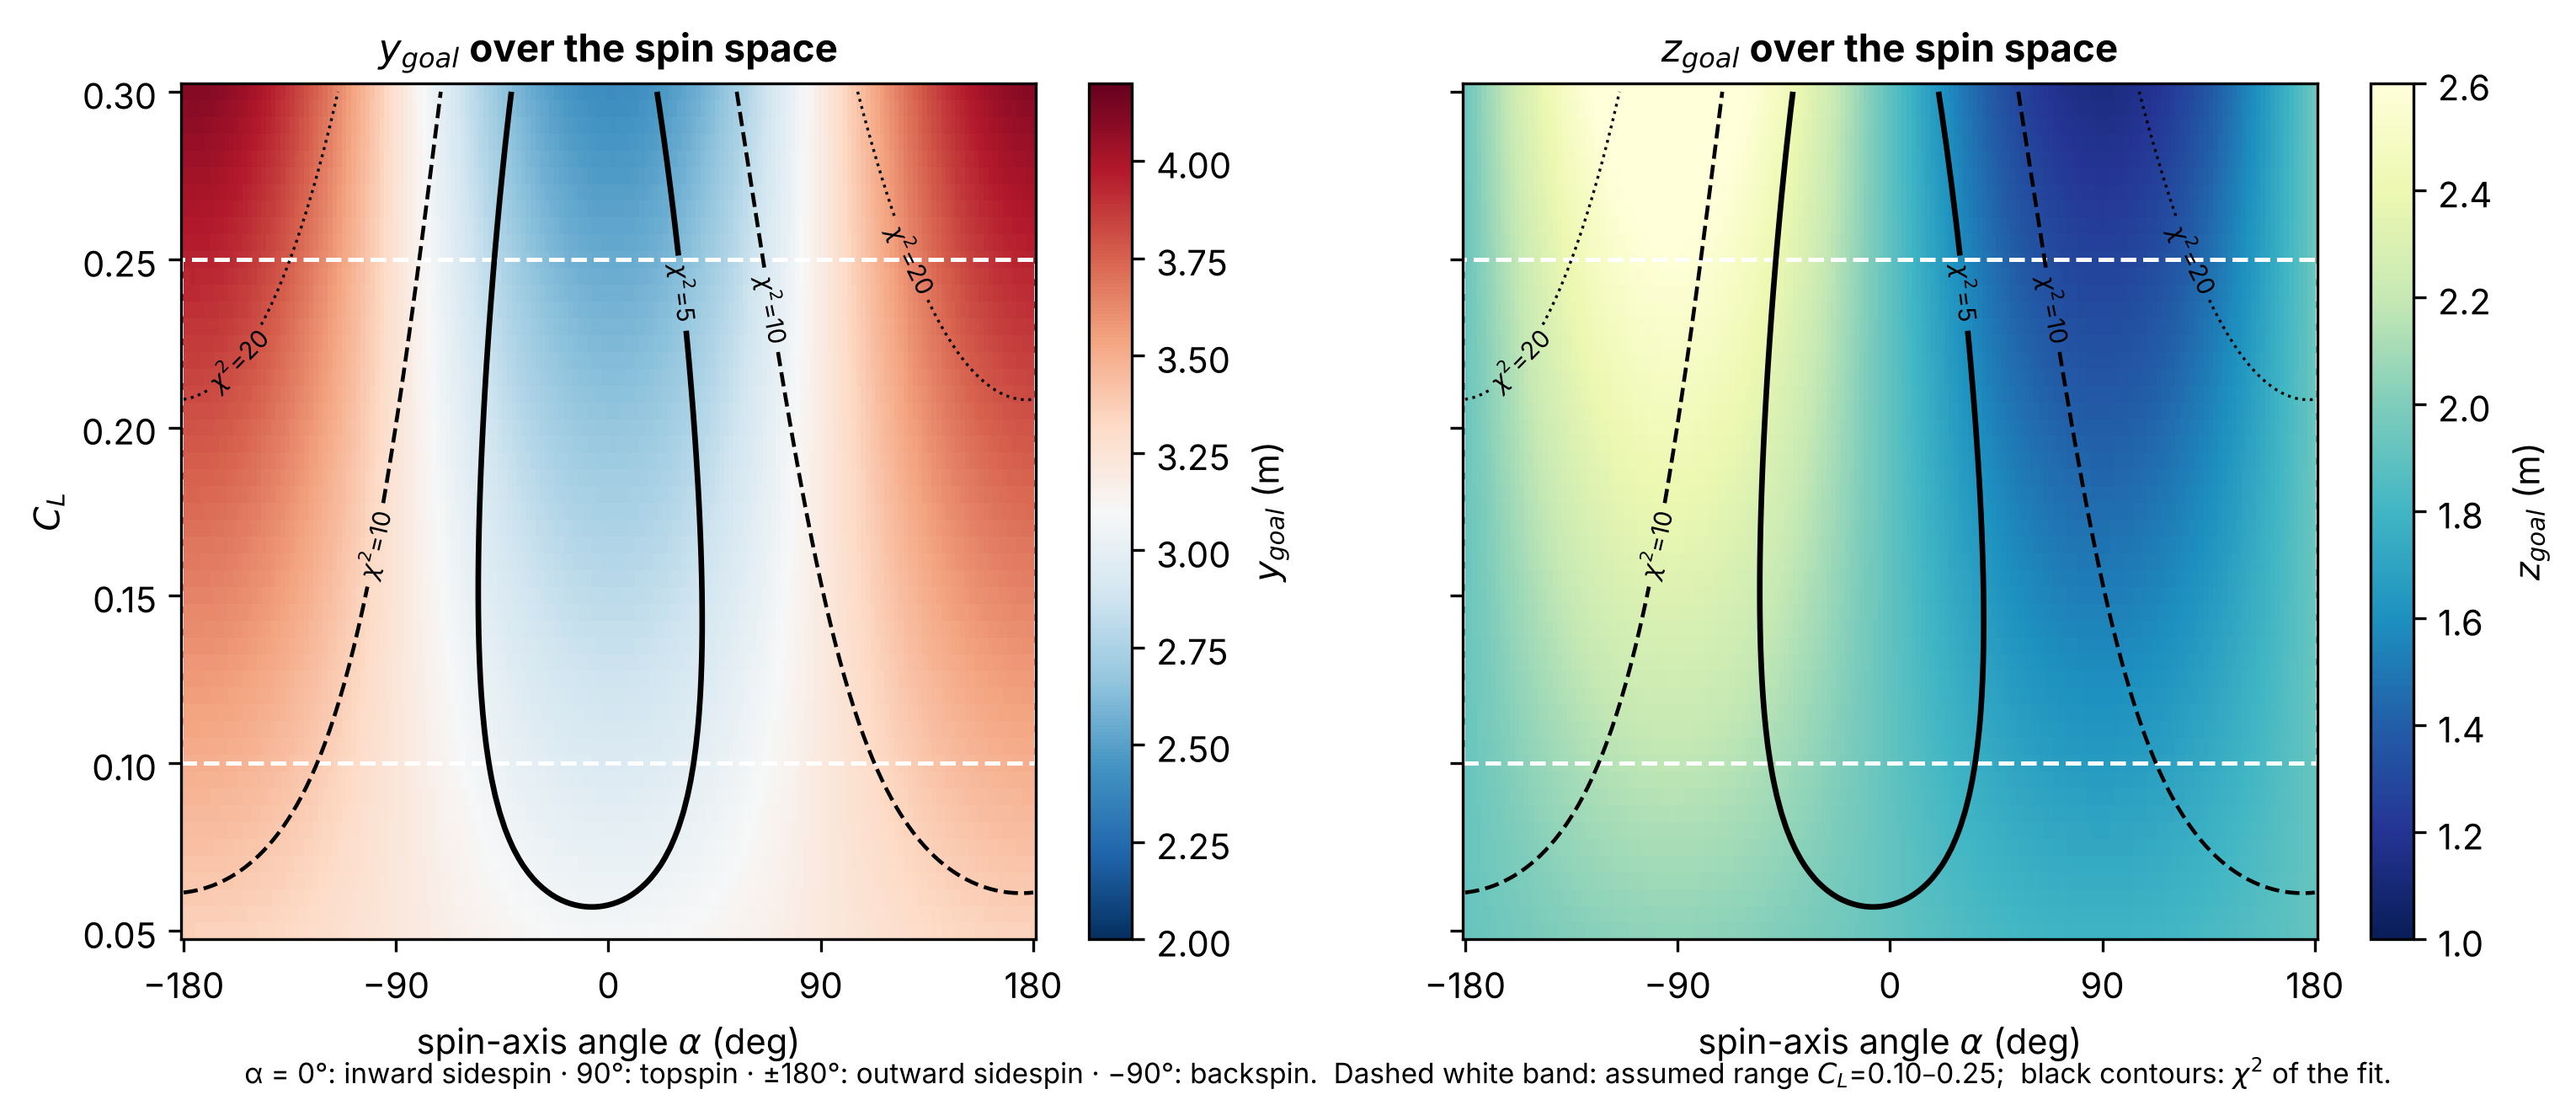
\includegraphics[width=\linewidth]{Figure/Heat_yz_maps.png}
    \caption{Predicted goal-plane coordinates $y_{\mathrm{goal}}$ 
    and $z_{\mathrm{goal}}$ across the spin-configuration space. 
    Black contours represent the $\chi^2$ fit levels, while the 
    dashed white boundaries indicate the assumed lift-coefficient 
    range $C_L\in[0.10,0.25]$. Even inside the $\chi^2=5$ contour $y_{\rm goal}$ changes by several tenths of a metre.}
    \label{fig:yzmaps}
\end{figure*}



\begin{table}[H]
\centering
\caption{Finite-difference acceleration estimate versus model accelerations at launch (m\,s$^{-2}$).}
\label{tab:fd}
\small
\begin{tabular}{lrrr}
\toprule
 & $a_x$ & $a_y$ & $a_z$\\
\midrule
Estimate from data ($\pm5.2$) & $-16$ & $-16$ & $-12$\\
Drag only ($C_D=0.22$) & $-11.3$ & $-3.3$ & $-12.4$\\
Drag + inward Magnus ($C_L=0.20$) & $-8.1$ & $-13.7$ & $-12.4$\\
\bottomrule
\end{tabular}
\end{table}

The vertical and longitudinal components are consistent with drag, but the lateral component $a_y$ is $2.4\sigma$ away from the no-spin prediction and $0.4\sigma$ from the inward-Magnus prediction. Using Eq.~\eqref{eq:ay}, $a_y\approx-3.32-51.5\,C_L$ (with $v_x=30.2$, $v_y=8.8$ m s$^{-1}$), so the measured value corresponds to $C_L\approx0.25\pm0.10$, a wide band (Figure~\ref{fig:fig10}). This diagnostic ignores coupling between channels; the full RK4 fit remains the reference.




\begin{figure*}[h!]
    \centering
    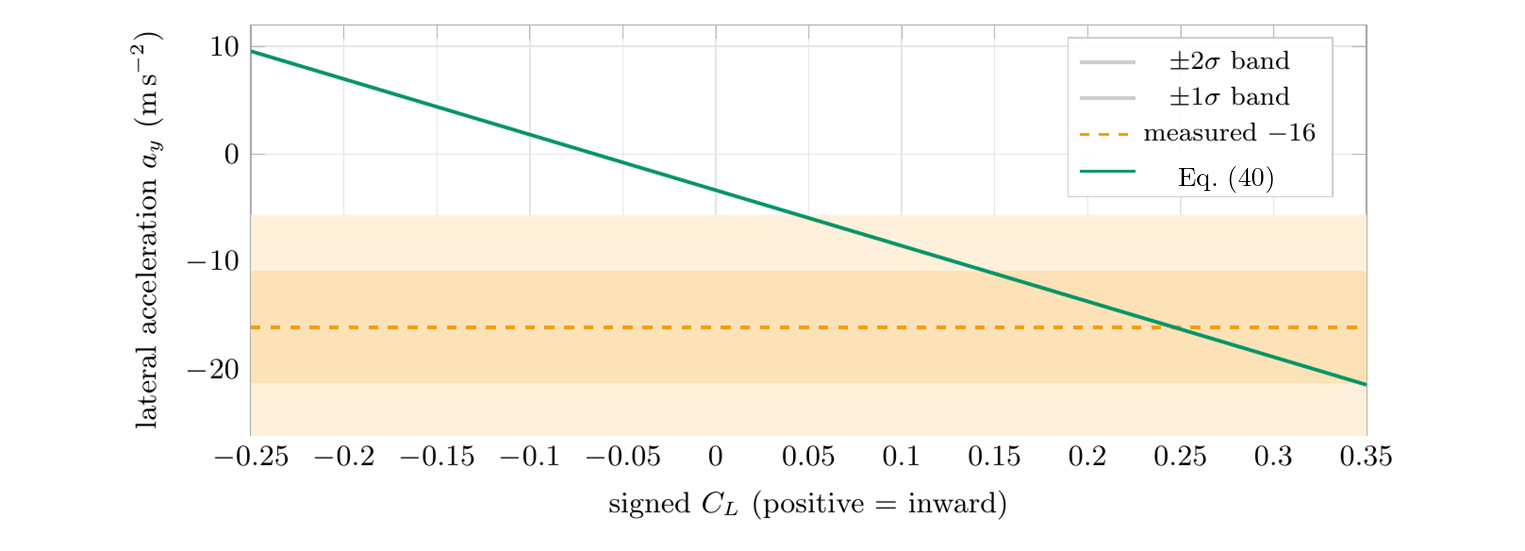
\includegraphics[width=5in]{Figure/Figure10.png}
    \caption{Model lateral acceleration versus CL compared with the finite-difference estimate
from the two observations.}
    \label{fig:fig10}
\end{figure*}




\subsection{Divergence of the fitted models after the data window}
The drag-only and inward-spin fits pass within about $\sigma$ of the data ($\chi^2\le7.8$, i.e.\ a root-mean-square residual of at most $\sqrt{7.8/6}\,\sigma\approx1.1\sigma$ per coordinate), so their differences in the first $0.1$ s are of the order of the measurement noise, but they diverge afterwards (Figure~\ref{fig:fig11}).


\begin{figure*}[h!]
    \centering
    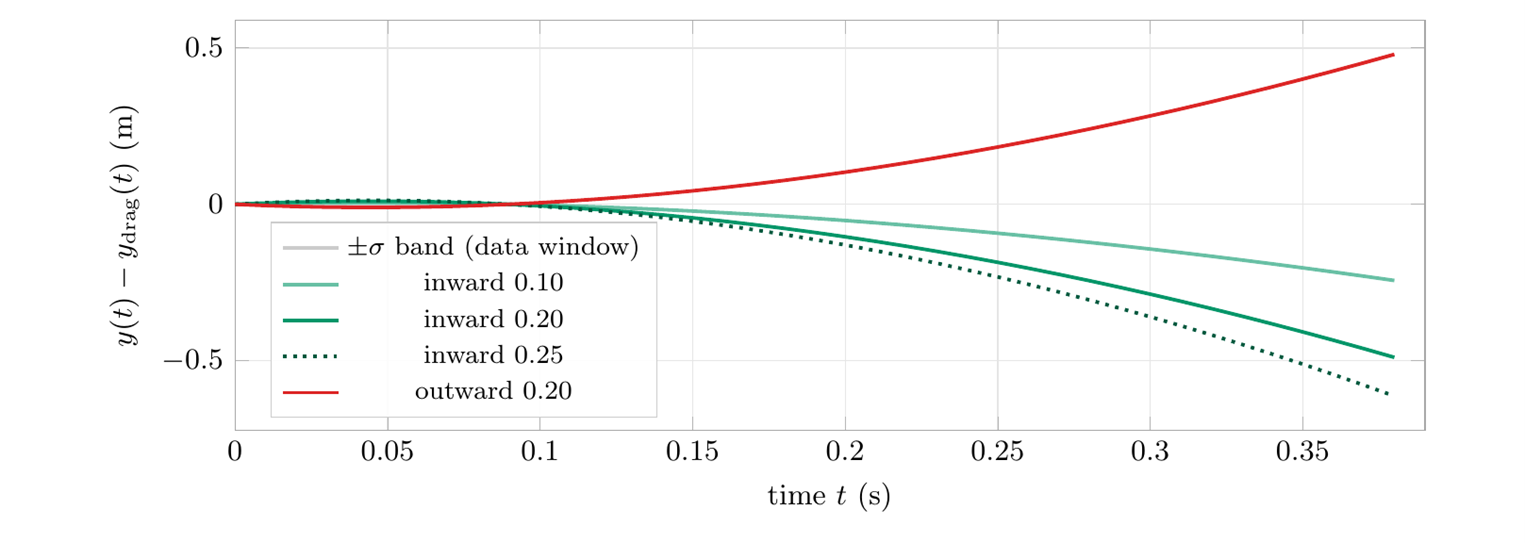
\includegraphics[width=5in]{Figure/Figure11.png}
    \caption{Lateral difference of each Magnus fit relative to the drag-only fit. Within the observation window ($t\le0.10$ s, grey band $\pm\sigma$) the curves are practically indistinguishable; at the goal plane they differ by $0.3$--$0.7$ m.}
    \label{fig:fig11}
\end{figure*}



\section{Interpretation of the Layered Physical Results}
Table~\ref{tab:physics} summarises the fixed-parameter layers.

The physical results support four observations. First, adding drag increases the flight time from approximately $0.371$ s to approximately $0.390$ s and lowers the predicted height by about $0.04$--$0.05$ m. Second, the lateral coordinate remains approximately unchanged under gravity and drag alone. Third, inward sidespin shifts the predicted lateral entry coordinate towards the centre, with the illustrative settings giving $y_{\rm goal}$ between $2.54$ m and $2.94$ m. Fourth, the opposite spin direction produces larger residual statistics for the tested settings. The data therefore favour inward curvature among the tested fixed configurations, but do not identify a unique lift coefficient.

\section{Probabilistic Prediction: Bayesian Ensemble (Method D)}
\label{sec:methodD}
The fixed-parameter layers above show that several spin configurations fit the two observations almost equally well. Instead of choosing one, our main method (Method D) treats the unknown aerodynamic parameters as random variables with literature-based priors and propagates the full set of plausible trajectories to the goal plane.

\subsection{Priors}
\begin{table}[H]
\centering
\caption{Prior distributions of the unknown parameters in Method D.}
\label{tab:priors}
\small
\begin{tabularx}{\linewidth}{@{}lXl@{}}
\toprule
Unknown & Prior & Source\\
\midrule
Kick type & 70\,\% instep, 30\,\% curve & assumption\\
Spin rate & instep $\mathcal N(3.25,0.8)$, curve $\mathcal N(7.35,1.0)$ rev/s, within $[0,10]$ & \citet{tsukada,asai2007}\\
Spin axis & instep: back/top-spin dominant; curve: axis elevation $\mathcal N(62.6^\circ,10^\circ)$ with a screw component & \citet{whiteside,tsukada}\\
Ball mass & $\mathcal U(0.410,0.450)$ kg & \citet{ifab}\\
$C_{D0}$ & $\mathcal U(0.15,0.20)$, plus $0.55\,Sp$ for spin & \citet{asai2007,goff2009}\\
$C_{L}$ & $C_{L,\max}(1-e^{-Sp/0.10})$, $C_{L,\max}\sim\mathcal U(0.25,0.35)$ & \citet{carre2002,goff2012}\\
\bottomrule
\end{tabularx}
\end{table}
Here $Sp=R\omega/\|\bm v_0\|$ is the spin parameter. In Method D the Magnus term is written as $s\,(\hat{\bm s}\times\bm v)$ with $s=k_L\|\bm v_0\|$ held constant during the flight.

\subsection{Algorithm}
\begin{enumerate}[leftmargin=*]
  \item Draw $N=2000$ parameter sets $(k_{D,i},s_i,\hat{\bm s}_i)$ from the priors.
  \item For each draw, fit $\bm v_{0,i}$ by Gauss--Newton least squares (Eq.~\eqref{eq:fit}) and record $\chi^2_i$.
  \item Assign likelihood weights $w_i\propto e^{-\chi^2_i/2}$, normalised to $\sum_i w_i=1$.
  \item Integrate each draw to $x=11$ m with RK4 ($\Delta t=1$ ms), giving $(y_i,z_i)$.
  \item The best-estimate entry point (posterior mean) and its covariance are
  \begin{equation}
    \bm\mu=\sum_i w_i(y_i,z_i),\qquad
    \mathbf C=\sum_i w_i\,\bm d_i\bm d_i^{\mathsf T},\quad \bm d_i=(y_i,z_i)-\bm\mu .
  \end{equation}
  The 68\,\% and 95\,\% regions are the ellipses $\bm d^{\mathsf T}\mathbf C^{-1}\bm d=2.279$ and $5.991$, and probabilities (e.g.\ of a goal) are sums of weights. The effective sample size is ${\rm ESS}=1/\sum_i w_i^2$.
\end{enumerate}
For each draw we keep the best-fit $\bm v_0$ instead of integrating over $\bm v_0$. Method D is therefore a likelihood-weighted ensemble with a profile-likelihood approximation for the launch velocity, rather than a full Bayesian posterior integration.

\subsection{Result for the given shot}
\begin{figure}[H]
  \centering
  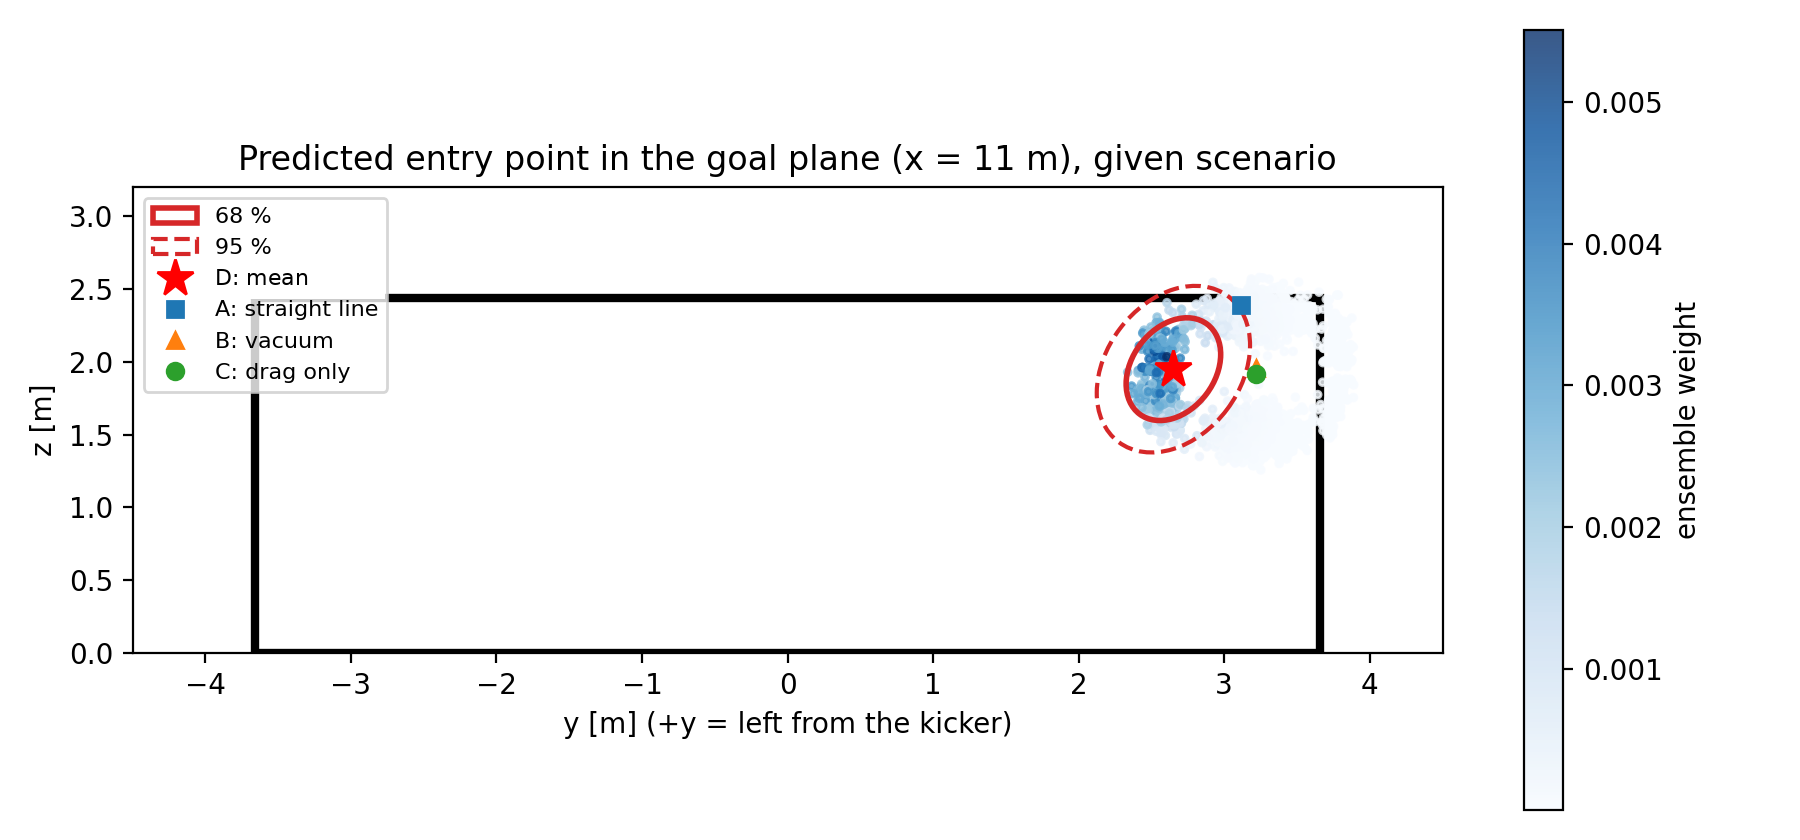
\includegraphics[width=0.85\linewidth]{Figure/fig_given_scenario.png}
  \caption{Method D for the given shot: weighted ensemble entry points (blue), posterior mean (star) and 68\,\%/95\,\% ellipses, with methods A--C for comparison.}
  \label{fig:given}
\end{figure}

\begin{table}[H]
\centering
\caption{Predicted entry point of the given shot.}
\label{tab:given}
\small
\begin{tabular}{@{}llll@{}}
\toprule
Method & $y_{\rm goal}$ (m) & $z_{\rm goal}$ (m) & Note\\
\midrule
A: straight line & 3.12 & 2.39 & no forces\\
B: gravity only & 3.22 & 1.96 & Layer 1\\
C: gravity + drag & 3.22 & 1.92 & Layer 2, $C_D=0.20$\\
\textbf{D: Bayesian ensemble} & $\mathbf{2.65\pm0.22}$ & $\mathbf{1.95\pm0.23}$ & $1\sigma$; corr.\ 0.29; ESS 393 of 2000\\
ML: gradient boosting & 2.74 & 2.04 & 68\,\%: $y\in[2.53,2.86]$, $z\in[1.67,2.25]$\\
\bottomrule
\end{tabular}
\end{table}
According to Method D, the centre of the ball enters the goal opening with probability 0.994, and the whole ball clears the posts and crossbar (radius 0.11 m, frame width 0.12 m) with probability 0.950. The posterior probability that the shot is a curve kick is 0.83 (prior 0.30), in line with the $\chi^2$ preference for inward spin in Table~\ref{tab:physics}. The posterior is bimodal: curve-kick draws centre near $y=2.57$ m and instep draws near $y=3.08$ m (Table~\ref{tab:sens}), so the mean of 2.65 m lies close to the dominant curve-kick mode (weighted mode 2.55 m). Because the 68\,\% ellipse covers only 54\,\% of curve kicks in our tests (Section~\ref{sec:testing}), the stated $\pm0.22$ m should be read as a lower bound; the sensitivity range $y=2.55$--$2.97$ m is a more conservative statement.

\subsection{Sensitivity of the answer}
\begin{table}[H]
\centering
\caption{Sensitivity of the Method D prediction for the given shot. Each row is an independent ensemble of 2000 draws; the baseline row therefore differs from Table~\ref{tab:given} ($y=2.65$ m, $P(\text{curve})=0.83$) only by Monte Carlo error.}
\label{tab:sens}
\small
\begin{tabular}{@{}lccc@{}}
\toprule
Setting & $y$ (m) & $z$ (m) & $P(\text{curve})$\\
\midrule
Curve-kick prior 10\,\% & 2.80 & 2.01 & 0.55\\
Curve-kick prior 30\,\% (baseline) & 2.67 & 1.96 & 0.81\\
Curve-kick prior 50\,\% & 2.61 & 1.94 & 0.91\\
Curve-kick prior 70\,\% & 2.59 & 1.93 & 0.96\\
\midrule
Assumed noise $\sigma=3.0$ mm & 2.55 & 1.97 & 1.00\\
Assumed noise $\sigma=10$ mm & 2.97 & 1.96 & 0.40\\
\midrule
Curve-kick draws only & 2.57 & 1.92 & weight 0.83\\
Instep draws only & 3.08 & 2.10 & weight 0.17\\
\bottomrule
\end{tabular}
\end{table}
The height is robust ($z=1.93$--$2.01$ m), whereas the lateral coordinate ranges from 2.55 to 2.97 m because it depends on whether the shot carries sidespin. The weighted mode (2.55, 1.95) m lies slightly inside the weighted mean. Repeating the ensemble with different random seeds changes $y$ by about 1.5 cm (Monte Carlo error).

\begin{figure}[H]
  \centering
  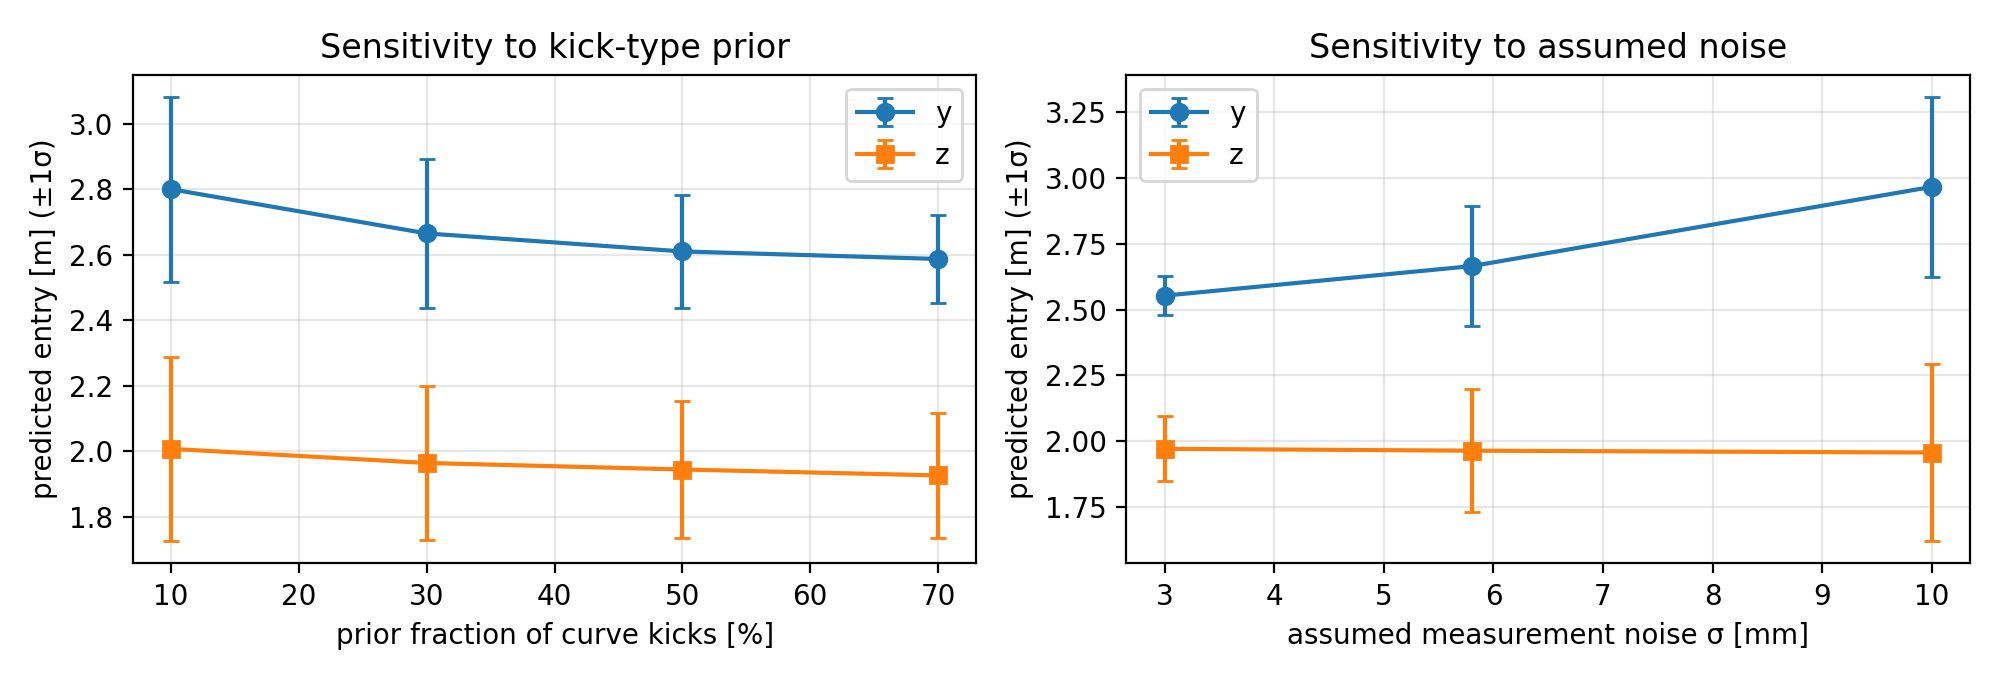
\includegraphics[width=0.9\linewidth]{Figure/fig_sensitivity.png}
  \caption{Sensitivity of the given-shot prediction to the kick-type prior and to the assumed noise ($\pm1\sigma$ bars).}
  \label{fig:sens}
\end{figure}

% nitu_spin.tex -- insert with % nitu_spin.tex -- insert with % nitu_spin.tex -- insert with \input{nitu_spin} at the end of the Method D section (just before \section{Testing the Methods}).
\subsection{What the observations reveal about the spin}
Figure~\ref{fig:spinpost} compares the prior and the likelihood-weighted posterior of the ensemble. The two observations shift the spin rate towards higher values (curve-kick range) and favour a spin axis that bends the ball towards the centre of the goal. The right panel shows why the lateral entry point is uncertain: $y_{\rm goal}$ is almost a linear function of the vertical component of the spin axis, i.e.\ of the amount of sidespin, which the first 0.10 s constrain only weakly. The weighted distribution of $y_{\rm goal}$ is therefore bimodal (curve and instep draws), while that of $z_{\rm goal}$ has a single peak (Figure~\ref{fig:marg}).

\begin{figure}[H]
  \centering
  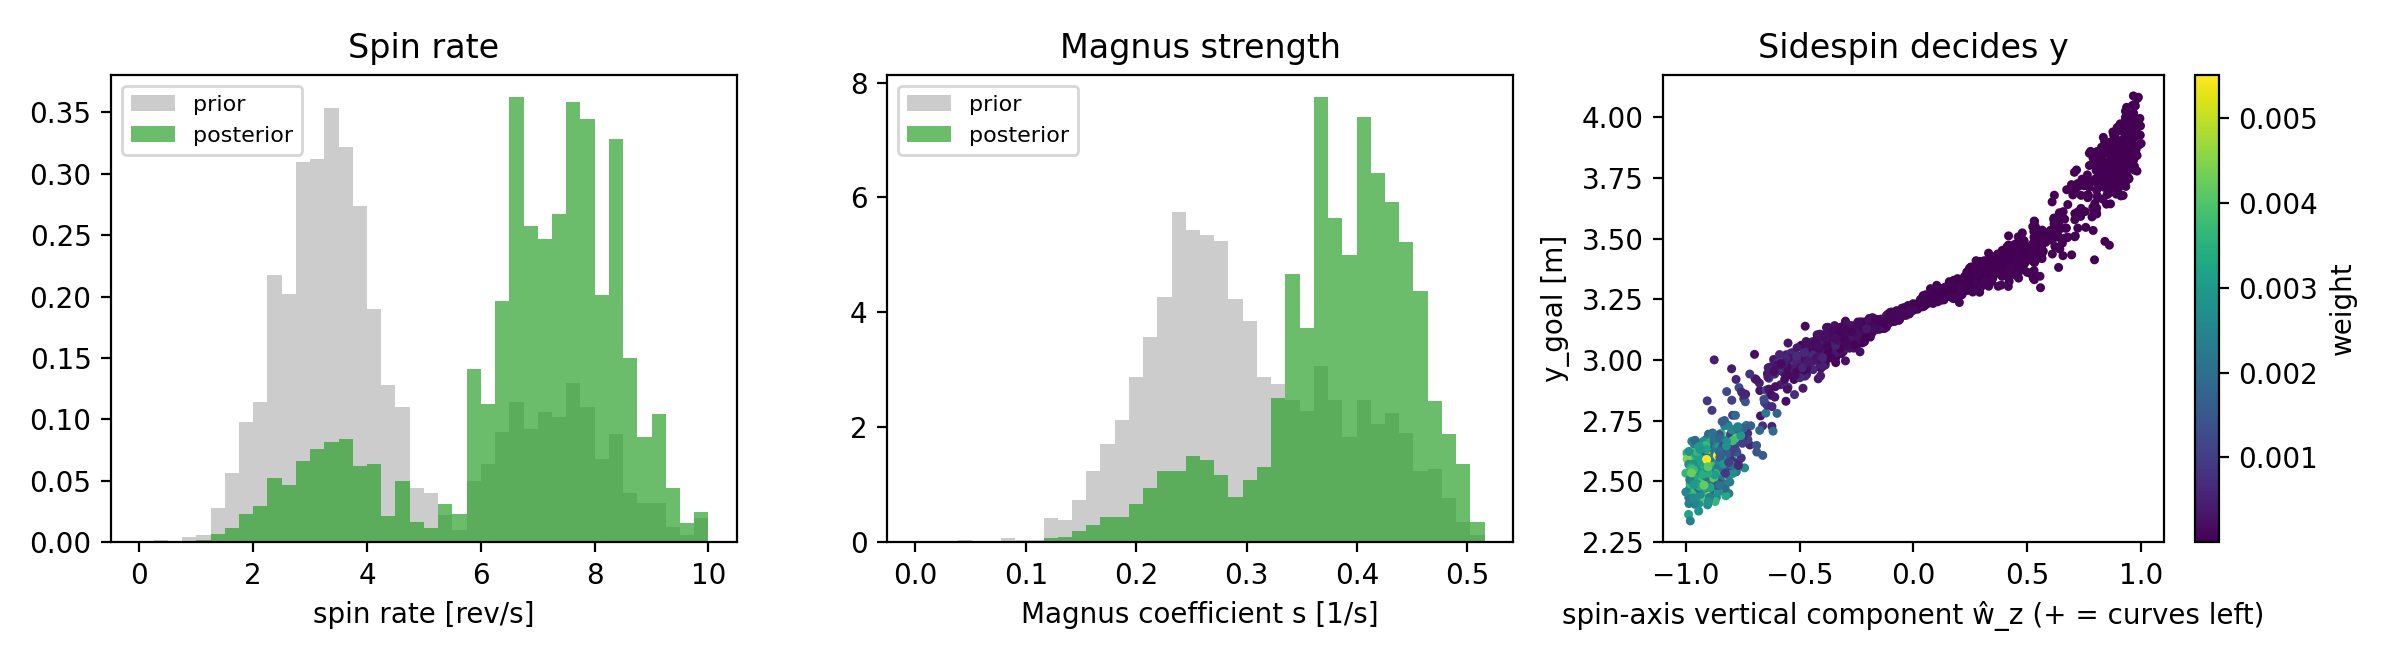
\includegraphics[width=\linewidth]{../penalty_dataset_v3/Model-D/fig_spin_posterior.png}
  \caption{Prior (grey) and posterior (green) of the spin rate and Magnus strength, and the dependence of the lateral entry point on the sidespin component of the spin axis (colour: weight).}
  \label{fig:spinpost}
\end{figure}

\begin{figure}[H]
  \centering
  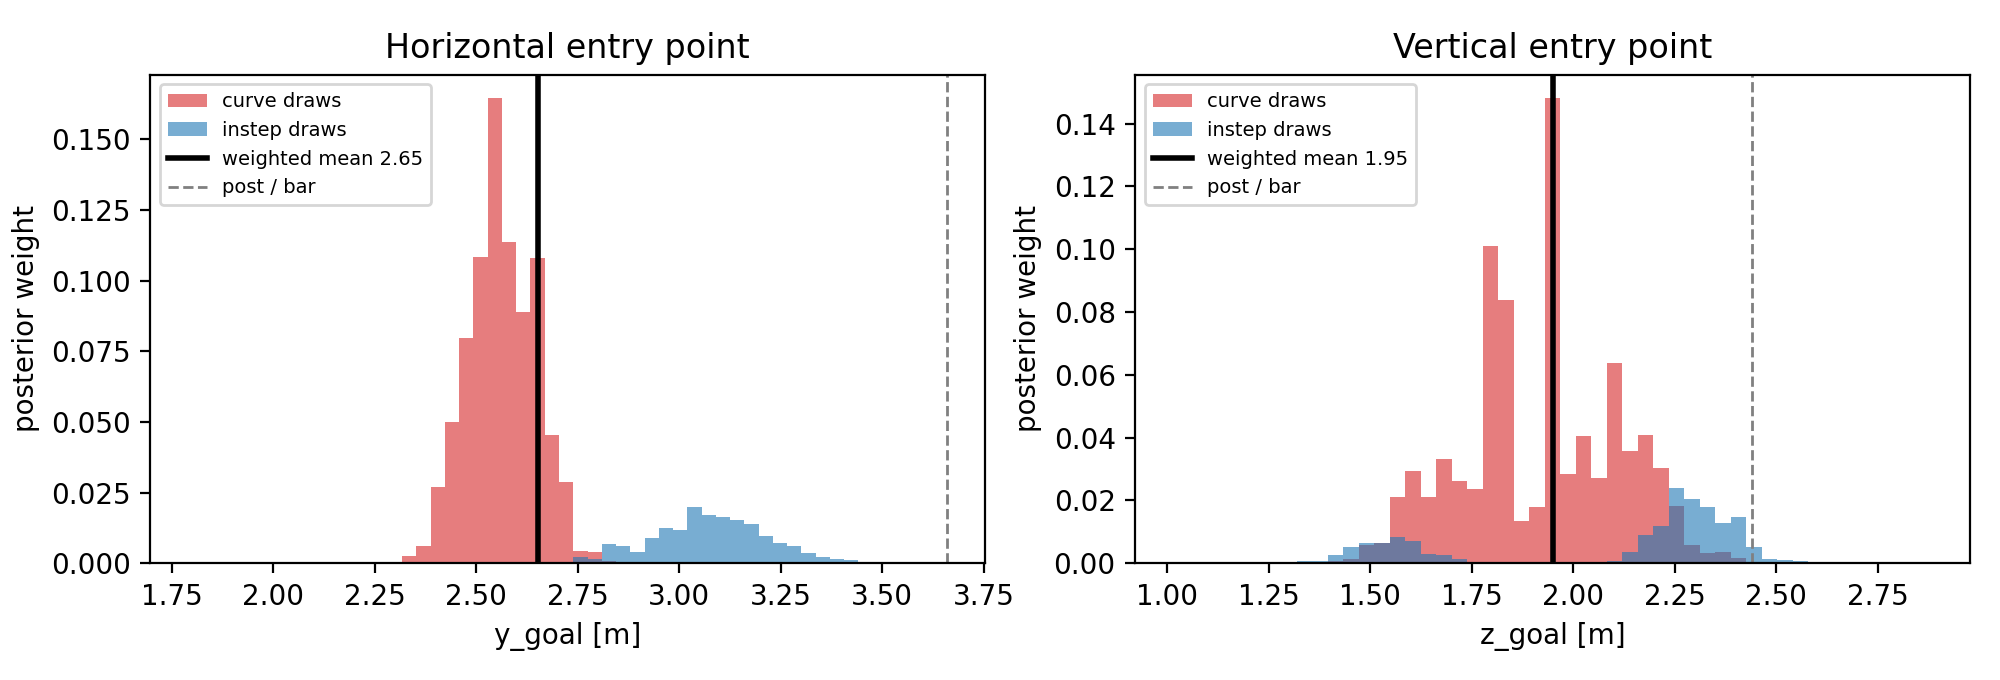
\includegraphics[width=\linewidth]{../penalty_dataset_v3/Model-D/fig_marginals.png}
  \caption{Weighted distributions of the entry point for the given shot, split into curve-kick and instep draws.}
  \label{fig:marg}
\end{figure}
 at the end of the Method D section (just before \section{Testing the Methods}).
\subsection{What the observations reveal about the spin}
Figure~\ref{fig:spinpost} compares the prior and the likelihood-weighted posterior of the ensemble. The two observations shift the spin rate towards higher values (curve-kick range) and favour a spin axis that bends the ball towards the centre of the goal. The right panel shows why the lateral entry point is uncertain: $y_{\rm goal}$ is almost a linear function of the vertical component of the spin axis, i.e.\ of the amount of sidespin, which the first 0.10 s constrain only weakly. The weighted distribution of $y_{\rm goal}$ is therefore bimodal (curve and instep draws), while that of $z_{\rm goal}$ has a single peak (Figure~\ref{fig:marg}).

\begin{figure}[H]
  \centering
  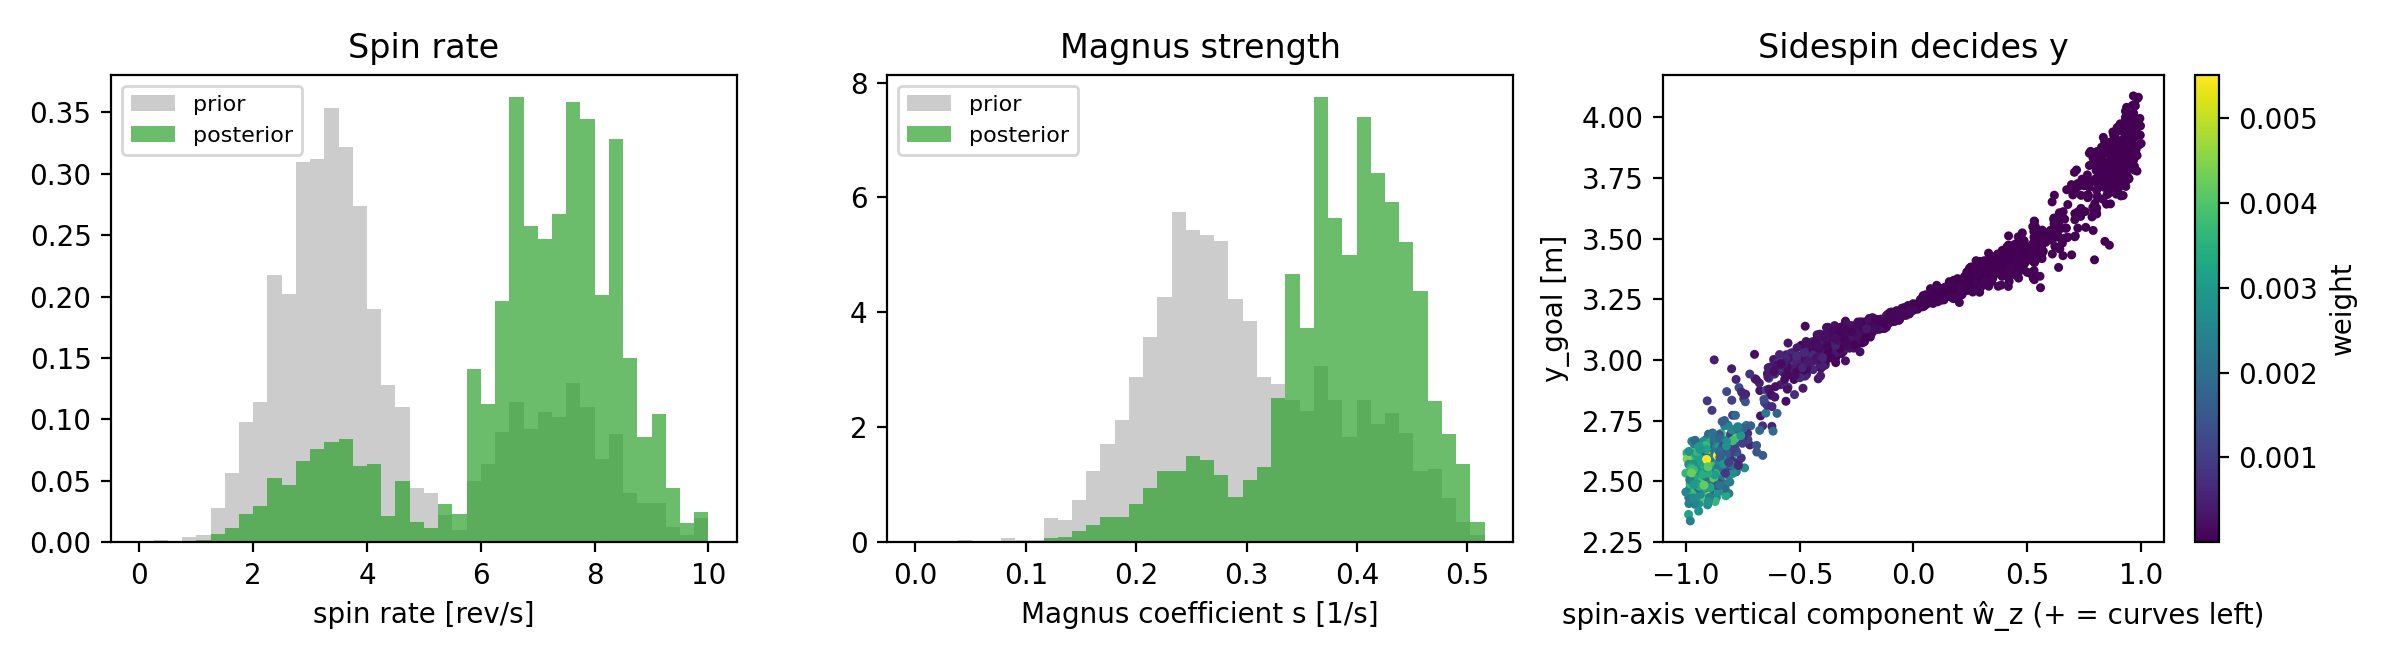
\includegraphics[width=\linewidth]{../penalty_dataset_v3/Model-D/fig_spin_posterior.png}
  \caption{Prior (grey) and posterior (green) of the spin rate and Magnus strength, and the dependence of the lateral entry point on the sidespin component of the spin axis (colour: weight).}
  \label{fig:spinpost}
\end{figure}

\begin{figure}[H]
  \centering
  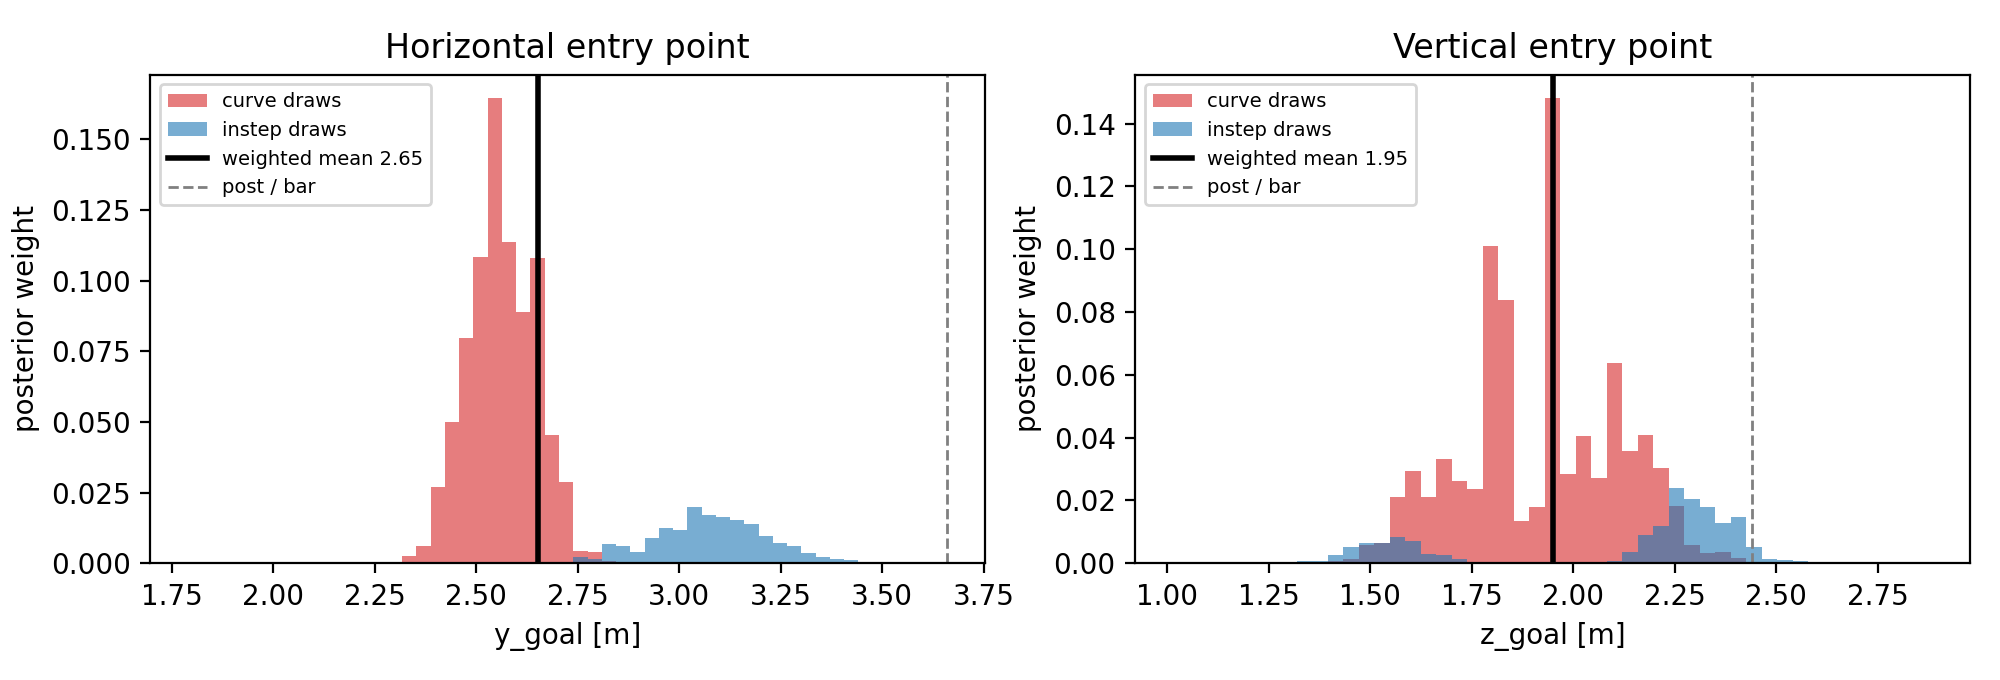
\includegraphics[width=\linewidth]{../penalty_dataset_v3/Model-D/fig_marginals.png}
  \caption{Weighted distributions of the entry point for the given shot, split into curve-kick and instep draws.}
  \label{fig:marg}
\end{figure}
 at the end of the Method D section (just before \section{Testing the Methods}).
\subsection{What the observations reveal about the spin}
Figure~\ref{fig:spinpost} compares the prior and the likelihood-weighted posterior of the ensemble. The two observations shift the spin rate towards higher values (curve-kick range) and favour a spin axis that bends the ball towards the centre of the goal. The right panel shows why the lateral entry point is uncertain: $y_{\rm goal}$ is almost a linear function of the vertical component of the spin axis, i.e.\ of the amount of sidespin, which the first 0.10 s constrain only weakly. The weighted distribution of $y_{\rm goal}$ is therefore bimodal (curve and instep draws), while that of $z_{\rm goal}$ has a single peak (Figure~\ref{fig:marg}).

\begin{figure}[H]
  \centering
  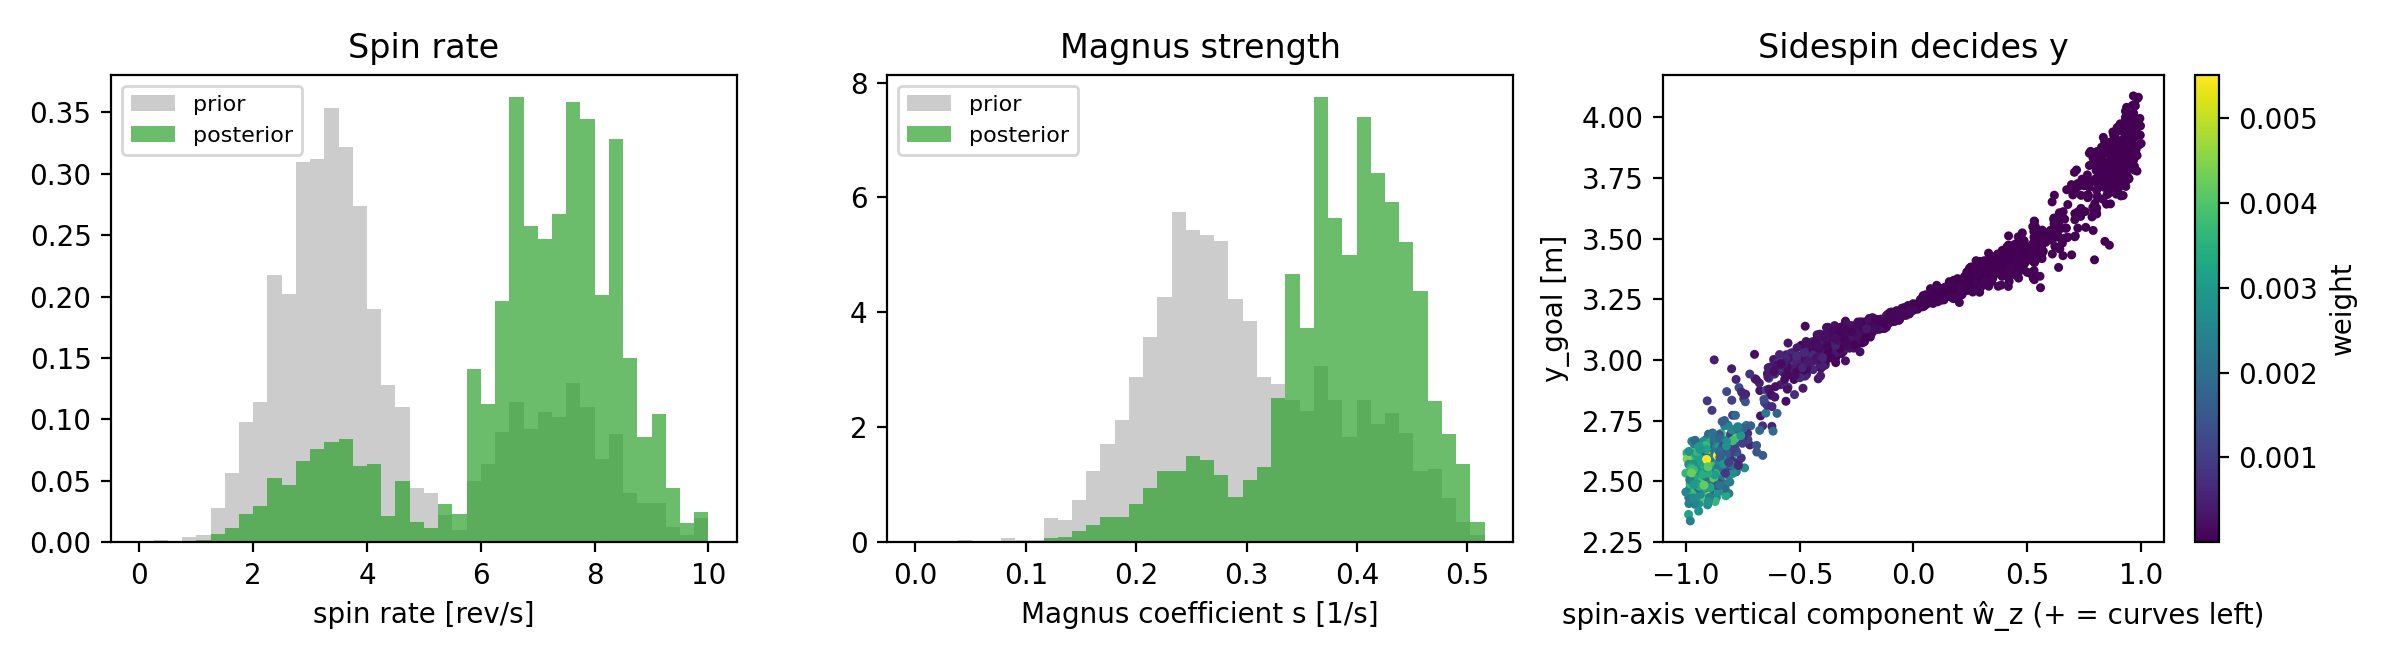
\includegraphics[width=\linewidth]{../penalty_dataset_v3/Model-D/fig_spin_posterior.png}
  \caption{Prior (grey) and posterior (green) of the spin rate and Magnus strength, and the dependence of the lateral entry point on the sidespin component of the spin axis (colour: weight).}
  \label{fig:spinpost}
\end{figure}

\begin{figure}[H]
  \centering
  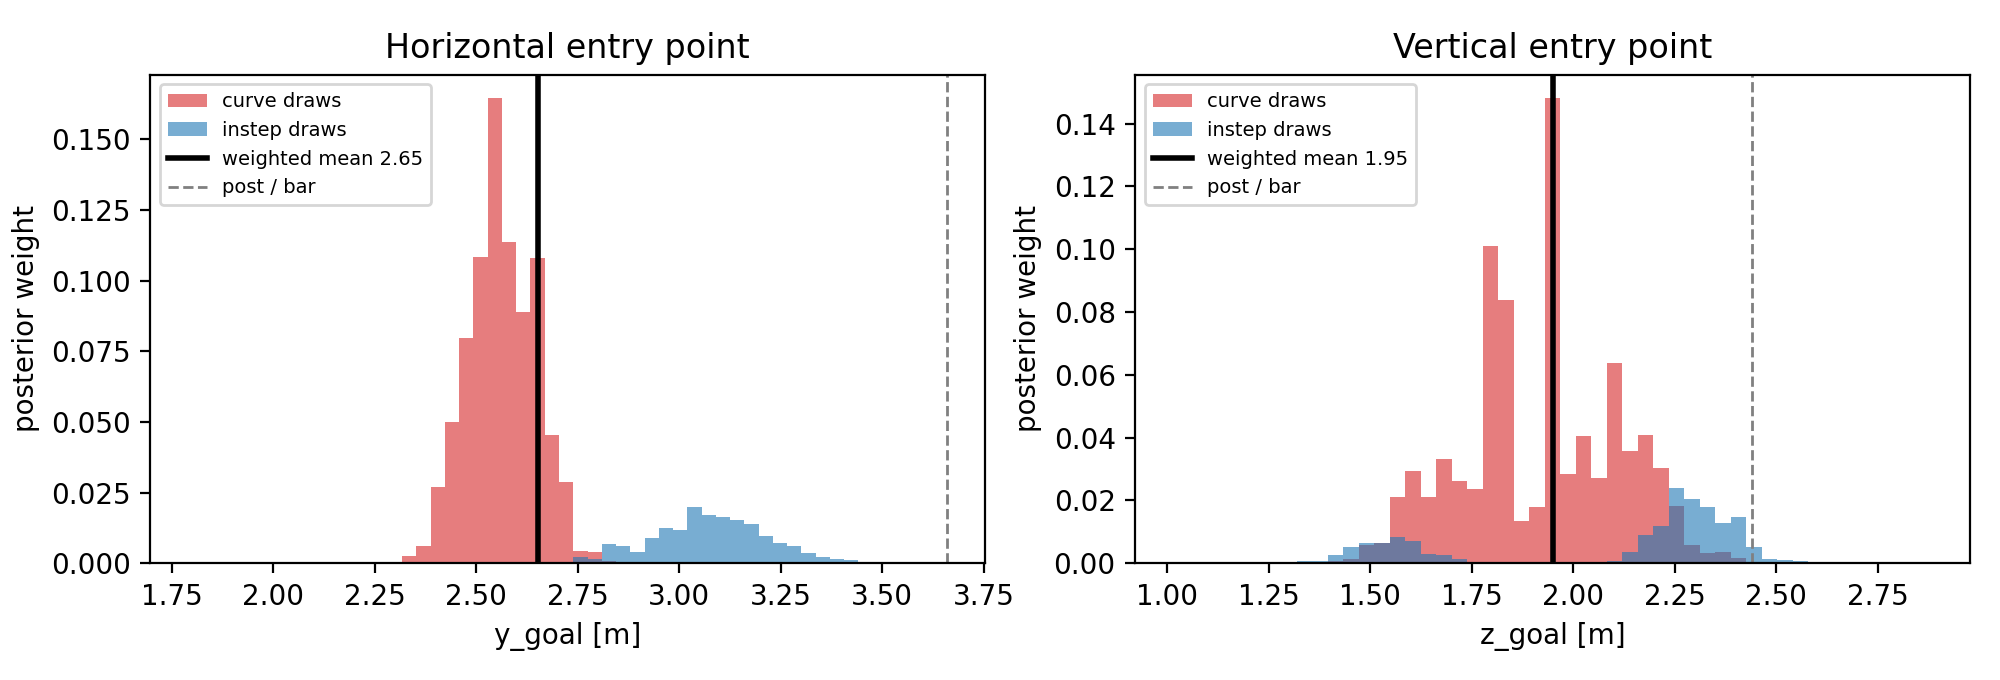
\includegraphics[width=\linewidth]{../penalty_dataset_v3/Model-D/fig_marginals.png}
  \caption{Weighted distributions of the entry point for the given shot, split into curve-kick and instep draws.}
  \label{fig:marg}
\end{figure}


\section{Testing the Methods}
\label{sec:testing}
\subsection{Test data}
The methods are tested on simulated penalties (60\,000 shots, split 70/15/15 into train, validation and test) with literature-based launch, spin and aerodynamic priors. The same shots are generated twice: with the simple model of Eq.~\eqref{eq:magnus} and with richer physics (speed-dependent drag from wind-tunnel fits \citep{goff2014}, spin-dependent lift, spin decay, wind up to 5 m/s and varying air density). Observations carry 5 mm Gaussian noise and are rounded to 0.01 m, like the given data; the combined error per coordinate is $\sqrt{5^2+10^2/12}\approx5.8$ mm, the value of $\sigma$ used throughout. We test on 300 test shots that reach the goal without bouncing; Method D uses no training data.

\subsection{Accuracy and calibration}
\begin{table}[H]
\centering
\caption{Goal-plane error on the same 300 test shots (cm).}
\label{tab:test}
\small
\begin{tabular}{@{}lcccc@{}}
\toprule
 & \multicolumn{2}{c}{Simple physics} & \multicolumn{2}{c}{Richer physics + wind}\\
\cmidrule(lr){2-3}\cmidrule(lr){4-5}
Method & median & 90th pct. & median & 90th pct.\\
\midrule
A: straight line & 64.0 & 119.0 & 63.6 & 117.7\\
B: gravity only & 48.3 & 72.3 & 44.8 & 70.2\\
C: gravity + drag & 48.8 & 70.7 & 45.5 & 72.0\\
\textbf{D: Bayesian ensemble} & \textbf{26.5} & \textbf{61.7} & \textbf{25.4} & \textbf{58.8}\\
ML: gradient boosting & 25.2 & 59.1 & 25.2 & 55.5\\
\bottomrule
\end{tabular}
\end{table}
Method D and the ML model reach statistically indistinguishable accuracy (Wilcoxon $p=0.20$, see below); we keep Method D as the main method because it needs no training data, uses the measurement noise explicitly and gives tested uncertainty regions. Method D halves the median error of the deterministic extrapolations and performs as well on the richer physics as on its own model. Its 68\,\% ellipse contains the true entry point in 69\,\% (simple) and 70\,\% (richer physics) of the shots, and its 95\,\% ellipse in 92\,\% and 93\,\%, so on shots drawn from the method's own prior the stated uncertainty is well calibrated, with slightly too small 95\,\% regions (Figure~\ref{fig:calib}).
Figure~\ref{fig:methoderr} shows the full error distributions: Method D shifts the whole distribution down, not only the median, while the straight-line extrapolation A has by far the widest spread.

\begin{figure}[H]
  \centering
  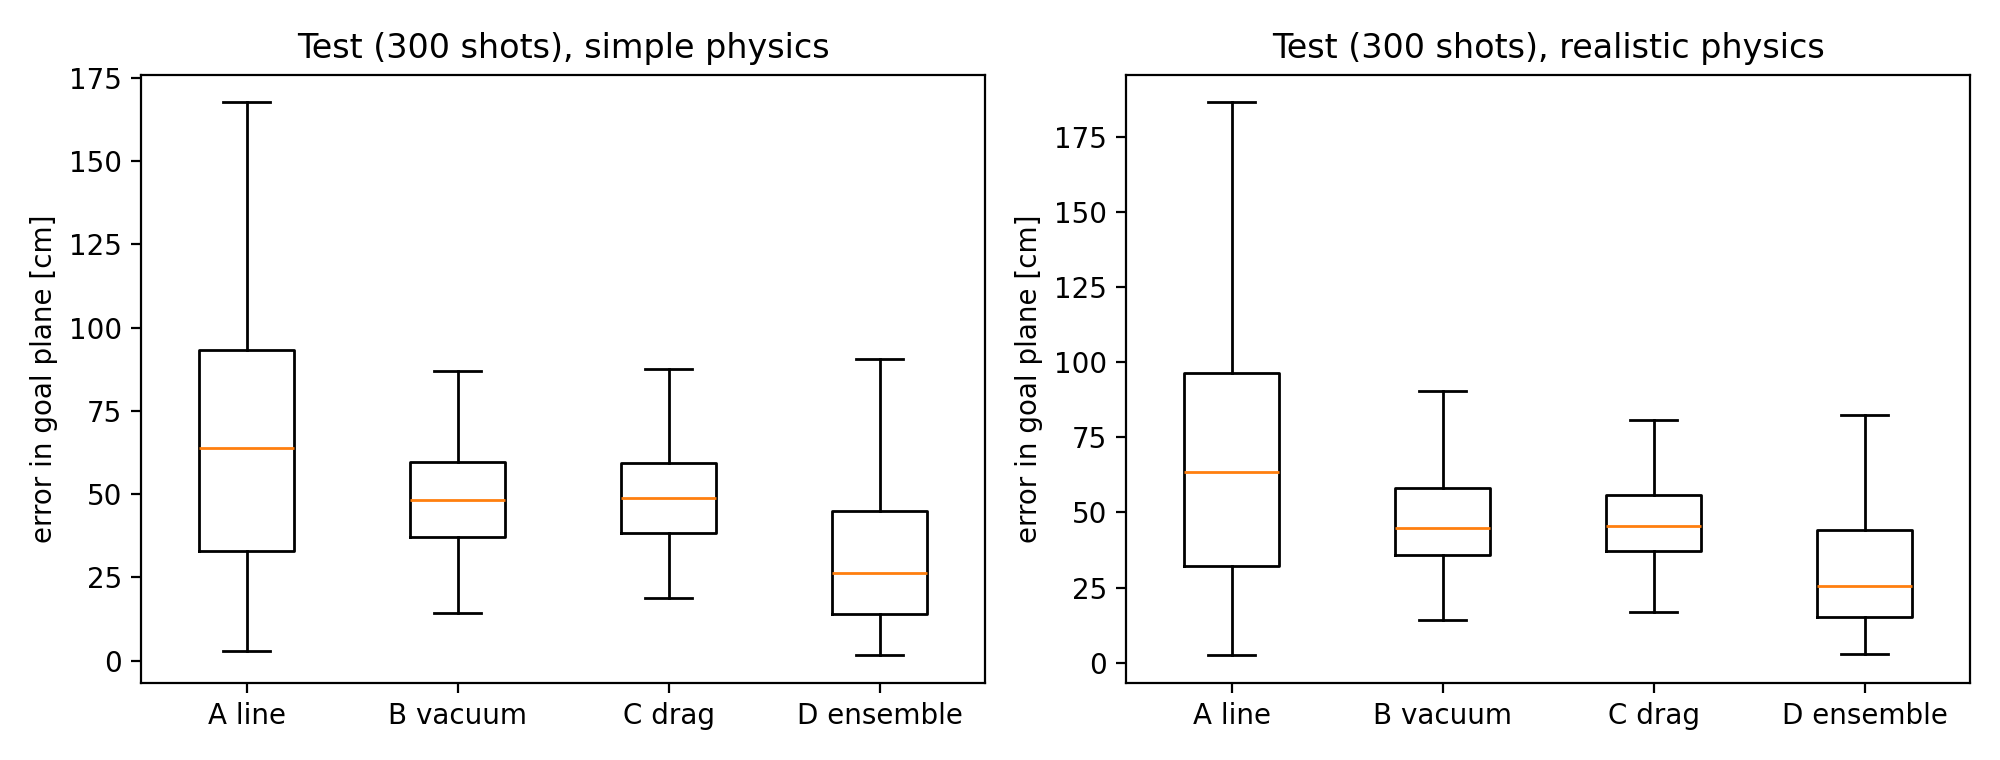
\includegraphics[width=\linewidth]{Figure/fig_method_errors.png}
  \caption{Goal-plane error of methods A--D on the same 300 test shots; left: simple physics, right: richer physics with wind. Boxes show the interquartile range, the orange line the median; whiskers extend to 1.5 times the interquartile range, outliers are not shown.}
  \label{fig:methoderr}
\end{figure}
\begin{figure}[H]
  \centering
  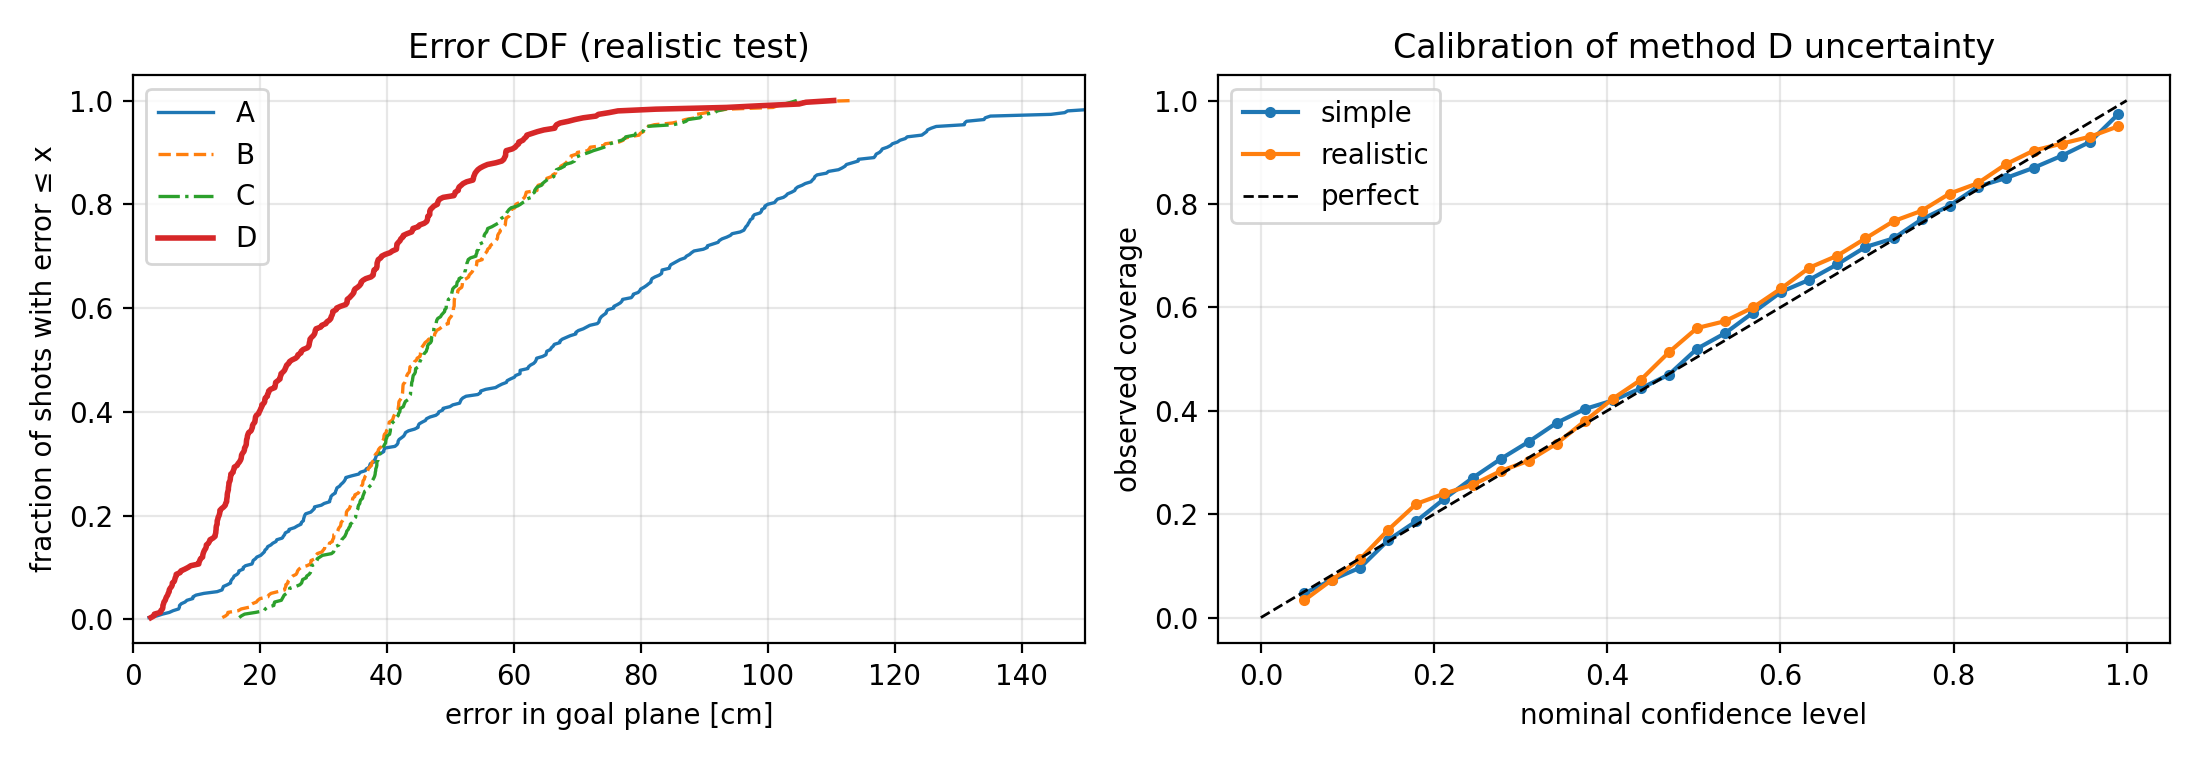
\includegraphics[width=\linewidth]{Figure/fig_cdf_calibration.png}
  \caption{Left: error distribution of methods A--D (richer physics). Right: observed vs nominal coverage of the Method D uncertainty.}
  \label{fig:calib}
\end{figure}

\subsection{What limits the accuracy?}
Three further checks on the same 300 test shots (simple / richer physics) show where the error comes from.

\emph{Curve kicks are the hard case.} Method D has a median error of 34 / 37 cm on the 82 curve kicks but 23 / 21 cm on the 218 instep kicks, and for curve kicks the error is mainly lateral (median $|\Delta y|\approx27$ cm vs.\ $|\Delta z|\approx16$ cm). The overall coverage hides a difference between the two groups: the 68\,\% ellipse contains the true point for 75--77\,\% of instep kicks but only 54\,\% of curve kicks. The stated uncertainty is therefore too small for strongly spinning shots, which applies to the given shot (posterior curve probability 0.83).

\emph{Slow shots are harder.} The median error falls from 44--45 cm for shots slower than 25 m/s to 18.5 cm for shots faster than 31 m/s, because a slow ball is exposed to drag and Magnus forces for longer after the observation window. The given shot ($\approx32$ m/s) lies in the most favourable speed range.

\emph{The limit is the data, not the method.} The errors of Method D and of the independently trained ML model are strongly correlated (correlation 0.89 / 0.91), their difference is not statistically significant (Wilcoxon signed-rank test, $p=0.20$ / $0.83$), and averaging the two predictions does not reduce the median error (26.0 / 25.4 cm). Both methods fail on the same shots, which indicates that an error of about 25 cm is set by the information in two early observations rather than by the choice of method, as the identifiability argument (seven unknowns, six measurements) predicts. The predicted uncertainty is nevertheless informative for individual shots: the error of Method D correlates with its stated $\sqrt{\sigma_y^2+\sigma_z^2}$ (correlation 0.50--0.52).

\subsection{Observation time, noise and bounced shots}
Observing the ball for longer reduces the Method D median error from 26 cm (last observation at 0.10 s) to 11 cm (0.15 s) and 5 cm (0.20 s), but the ellipses then become too narrow (68\,\% coverage 56--60\,\%, from 150 shots each). With the method's assumed noise matched to the true noise, the median error grows from 11 cm ($\sigma=2$ mm) to 48 cm ($\sigma=20$ mm). Shots that bounce before the goal are predicted poorly (median 50 cm), because the flight model ignores ground contact.

\begin{figure}[H]
  \centering
  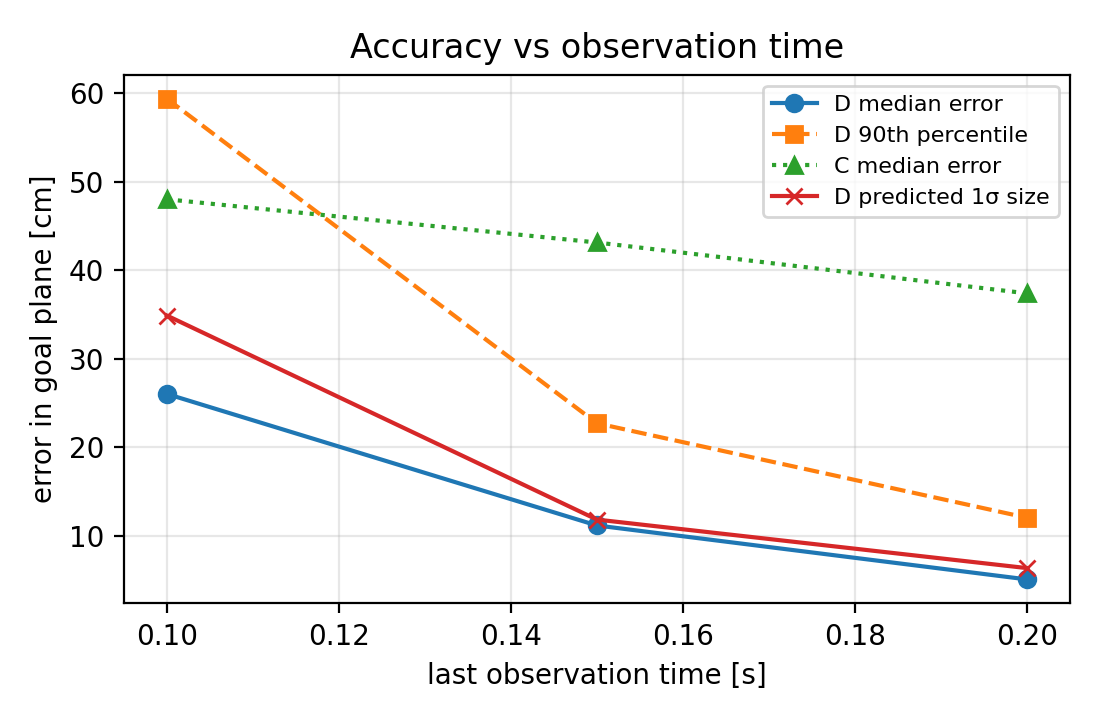
\includegraphics[width=0.7\linewidth]{Figure/fig_accuracy_vs_time.png}
  \caption{Method D error versus the time of the last observation.}
  \label{fig:time}
\end{figure}

\section{Machine-Learning Method}

\subsection{Data preparation and target definition}
The machine-learning model uses the two simulated datasets described in Section~\ref{sec:testing}: one generated with the simple model and one with richer physics. The simple dataset is used to construct the train and validation sets; the realistic dataset is used as a separate test domain. Regression training retains shots that reach the goal plane without bouncing. Final clean test evaluation is restricted to on-target shots that do not bounce before reaching the goal plane.

The two regression targets are trained separately:
\begin{equation}
    f_y:\bm x\mapsto y_{\rm goal},\qquad
    f_z:\bm x\mapsto z_{\rm goal}.
\end{equation}
The random seed is fixed to 42. The essential code is given in Appendix~A; the complete notebooks and simulated datasets are available from the team on request.

\subsection{Feature engineering}
All features are derived from the six observed coordinates and the known initial position $\bm p_0=(0,0,0.11)$. Let $\bm p_1=\bm r(t_1)$ and $\bm p_2=\bm r(t_2)$. The two interval velocities and finite-difference acceleration are
\begin{align}
    \bm v_1&=\frac{\bm p_1-\bm p_0}{0.05},&
    \bm v_2&=\frac{\bm p_2-\bm p_1}{0.05},\\
    \bm a&=\frac{\bm v_2-\bm v_1}{0.05}.
\end{align}
The 23-dimensional feature vector contains:
\begin{itemize}[leftmargin=*]
    \item six raw position coordinates ($\bm p_1,\bm p_2$);
    \item six velocity components ($\bm v_1,\bm v_2$);
    \item three acceleration components ($\bm a$);
    \item speed, azimuth, and elevation for each interval (six features);
    \item linear-extrapolation estimates of $y$ and $z$ at $x=11$ m (two features).
\end{itemize}
For the last two features, the second interval velocity is extrapolated to the goal plane:
\begin{align}
    \Delta t_g&=\frac{11-p_{2x}}{v_{2x}},\\
    y_{\rm lin}&=p_{2y}+v_{2y}\Delta t_g,\qquad
    z_{\rm lin}=p_{2z}+v_{2z}\Delta t_g.
\end{align}
Hence, the model receives no hidden future trajectory information; all 23 inputs are deterministic transformations of the same six measured coordinates.

\subsection{Candidate regressors and model selection}
Three model families are compared:
\begin{enumerate}[leftmargin=*]
    \item \textbf{Ridge regression:} standardised features followed by linear ridge regression with $\alpha=1$;
    \item \textbf{MLP:} a feed-forward multilayer perceptron with hidden layers $(128,64)$, early stopping, and at most 400 iterations;
    \item \textbf{Histogram gradient boosting (HGB):} up to 600 boosting iterations, learning rate $0.06$, and at most 63 leaf nodes.
\end{enumerate}
For each candidate, separate models are fitted for $y_{\rm goal}$ and $z_{\rm goal}$. Model selection is performed using the validation set only. The validation error for an on-target validation shot is the Euclidean error in the goal plane:
\begin{equation}
    e_i=\sqrt{(\widehat y_i-y_i)^2+(\widehat z_i-z_i)^2}.
\end{equation}
The selected model minimises the validation median error; the 90th percentile is also reported.

\subsection{Quantile-based uncertainty}
We fit HGB quantile regressors for each target at
\begin{equation}
    \mathcal Q=\{0.025,0.16,0.50,0.84,0.975\}.
\end{equation}
The interval between the 16th and 84th percentiles is treated as an approximate central 68\% prediction interval, and the 2.5th--97.5th percentile interval as a central 95\% interval. Predicted quantiles are sorted for each sample to prevent quantile crossing. Empirical coverage is calculated separately for each axis and jointly for the rectangular two-axis region.

\subsection{Evaluation protocol}
We report results on (i) the clean simple test set and (ii) the clean realistic test set. Metrics include median and 90th-percentile Euclidean error in centimetres, per-axis 68\% and 95\% coverage, and joint rectangular coverage. Comparisons with Method D use the same test shots. Additional analyses include error cumulative distribution functions, goal-zone error, performance versus observation time, noise sensitivity, bounced-shot evaluation, and extrapolation to higher-speed shots. The results are given in Section~\ref{sec:testing} and in the machine-learning results below.

\section{Machine-Learning Results}
On the validation set, gradient boosting (median 25.2 cm) narrowly beats the MLP (25.4 cm) and ridge regression (29.7 cm) and is selected. Table~\ref{tab:mlresults} gives the results on the full clean test sets.

\begin{table}[H]
\centering
\caption{Machine-learning performance on the clean test sets (selected model: HGB).}
\label{tab:mlresults}
\small
\begin{tabular}{@{}lccccc@{}}
\toprule
Test domain & $n$ & Median (cm) & P90 (cm) & 68\,\% coverage ($y,z$) & 95\,\% coverage ($y,z$)\\
\midrule
Simple & 4921 & 25.0 & 58.4 & 0.64, 0.65 & 0.90, 0.91\\
Richer physics & 4894 & 24.4 & 56.2 & 0.65, 0.66 & 0.91, 0.91\\
\bottomrule
\end{tabular}
\end{table}

For the given shot the model predicts $(\widehat y_{\rm ML},\widehat z_{\rm ML})=(2.74,\,2.04)$ m with 68\,\% intervals $y\in[2.53,2.86]$ m and $z\in[1.67,2.25]$ m, and a goal probability of 0.96. This lies inside the 68\,\% ellipse of Method D (Figure~\ref{fig:mlvsd}), so two independent approaches agree.

\begin{figure}[H]
  \centering
  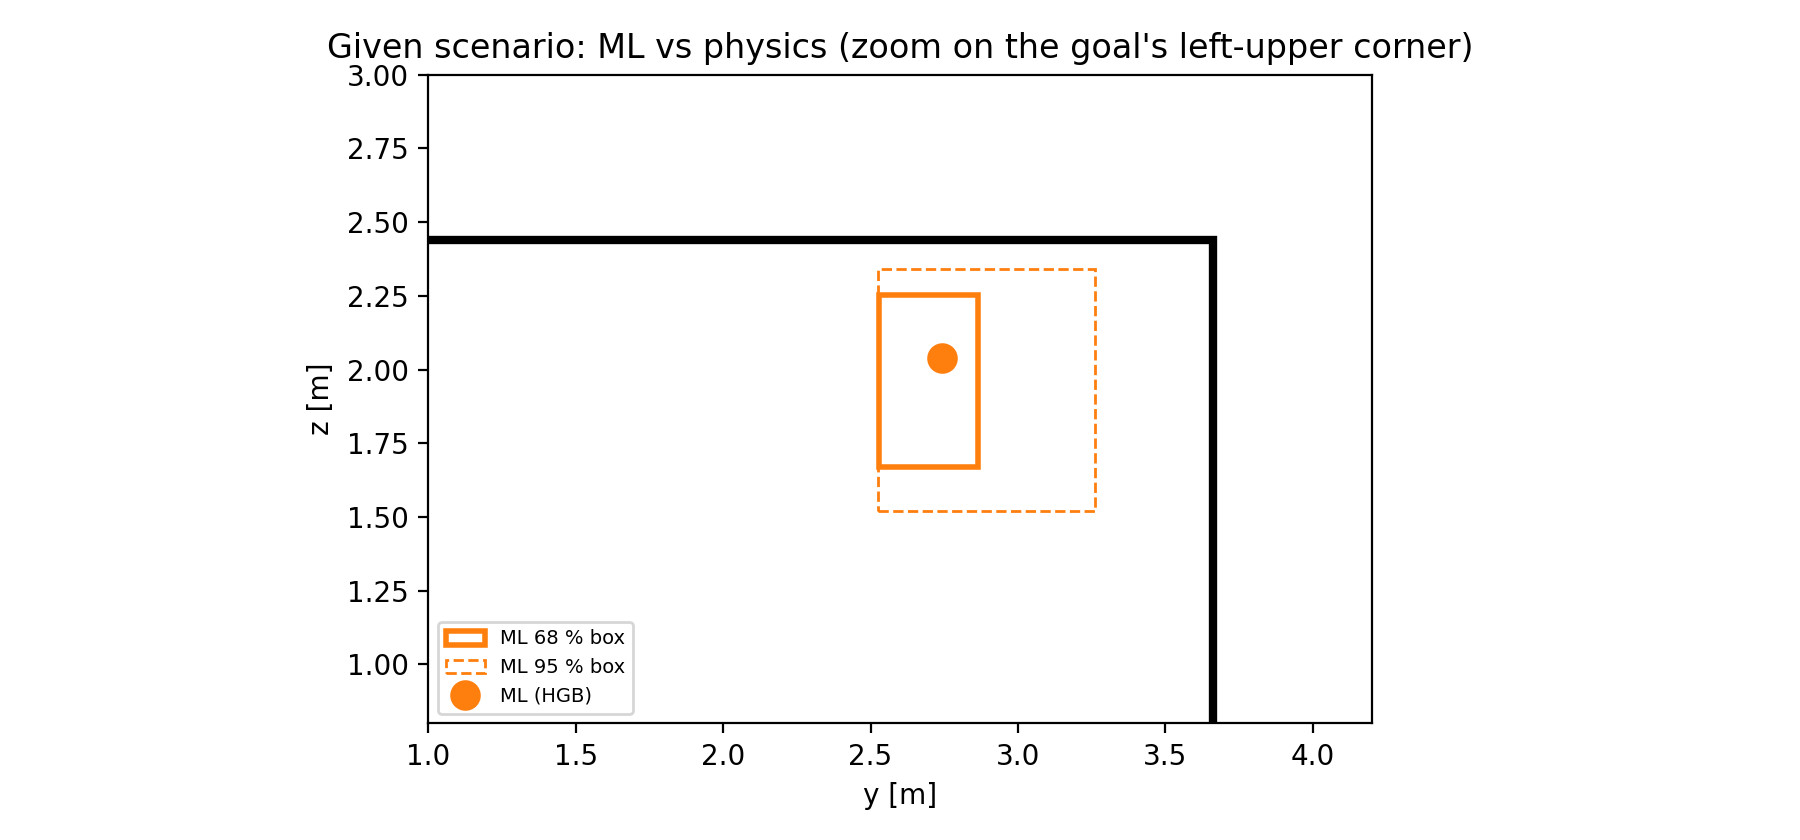
\includegraphics[width=0.8\linewidth]{Figure/fig_ml_vs_D_given.png}
  \caption{Given shot: ML prediction with 68/95\,\% boxes and Method D with 68/95\,\% ellipses.}
  \label{fig:mlvsd}
\end{figure}

On the same 300 test shots ML and Method D are equally accurate (Table~\ref{tab:test}). Three differences matter. (i) When trained only on slower shots (speed $<30$ m/s) and tested on faster ones ($>33$ m/s), the ML median error rises from 16.1 to 20.3 cm, whereas Method D needs no training range. (ii) ML intervals are learned at one noise level: at $\sigma=20$ mm its 68\,\% coverage drops to about 0.31, while Method D can use the assumed noise explicitly. (iii) On bounced shots ML is better (median 26 cm vs about 50 cm), because it never predicts a crossing below ground level.

% nitu_compare.tex -- insert with % nitu_compare.tex -- insert with % nitu_compare.tex -- insert with \input{nitu_compare} after the Machine-Learning Results section (just before \section{Goalkeeper Reach Analysis}).
\section{Further Comparison of Method D and Machine Learning}
\subsection{Observation time}
\begin{table}[H]
\centering
\caption{Median (90th percentile) goal-plane error versus the time of the last observation (cm). Method D: 150 test shots; ML retrained for each window, full clean test set.}
\label{tab:time}
\small
\begin{tabular}{@{}lccc@{}}
\toprule
Last observation & C: gravity + drag & D: Bayesian ensemble & ML: gradient boosting\\
\midrule
0.10 s & 48.0 & 26.0 (59.4) & 24.9 (58.5)\\
0.15 s & 43.1 & 11.2 (22.7) & 11.1 (25.6)\\
0.20 s & 37.4 & \phantom{0}5.1 (12.1) & \phantom{0}6.3 (13.8)\\
\bottomrule
\end{tabular}
\end{table}
One extra observation at 0.15 s more than halves the error of both D and ML, while the drag-only fit improves only slightly: its error is dominated by the missing spin. For a goalkeeper this means that each additional 0.05 s of watching the ball is very valuable.

\subsection{Robustness to measurement noise}
\begin{table}[H]
\centering
\caption{Median goal-plane error (cm) and 68\,\% coverage for different measurement noise. D assumes the true $\sigma$ for i.i.d.\ noise and $\sigma=5.8$ mm otherwise; ML was trained once at 5 mm noise. D: 100 shots per row; ML: full clean test subset.}
\label{tab:noise}
\small
\begin{tabular}{@{}lcccc@{}}
\toprule
Noise & D median & D 68\,\% cov. & ML median & ML 68\,\% cov.\ ($y$, $z$)\\
\midrule
i.i.d.\ 2 mm & 11.0 & 0.62 & 19.0 & 0.73, 0.76\\
i.i.d.\ 5 mm & 21.7 & 0.69 & 23.7 & 0.64, 0.65\\
i.i.d.\ 10 mm & 35.9 & 0.75 & 34.4 & 0.49, 0.49\\
i.i.d.\ 20 mm & 48.4 & 0.63 & 54.8 & 0.30, 0.33\\
$x$ noise $\times3$ & 29.6 & 0.66 & 24.5 & 0.63, 0.65\\
1 ms timing jitter & 30.4 & 0.70 & 25.8 & 0.61, 0.60\\
5\,\% outliers & 26.9 & 0.74 & 25.1 & 0.62, 0.62\\
\bottomrule
\end{tabular}
\end{table}
When the noise level is known, Method D adapts: it is clearly more accurate than ML for precise measurements (11 vs 19 cm at 2 mm) and its coverage stays between 0.62 and 0.75, whereas the ML intervals, learned at one noise level, cover only about 30\,\% of the cases at 20 mm. When the noise has a different structure than assumed (anisotropic, timing jitter, outliers), ML is slightly more accurate, but Method D keeps a reasonable coverage.

\subsection{Where in the goal is prediction hardest?}
Across the $3\times3$ goal zones the median error of Method D ranges from 20 cm (high centre) to 35 cm (high, kicker's right) and 32 cm (low, kicker's left), with about 30 test shots per zone; ML shows the same range (18--33 cm). No zone is predicted dramatically worse than the others.
 after the Machine-Learning Results section (just before \section{Goalkeeper Reach Analysis}).
\section{Further Comparison of Method D and Machine Learning}
\subsection{Observation time}
\begin{table}[H]
\centering
\caption{Median (90th percentile) goal-plane error versus the time of the last observation (cm). Method D: 150 test shots; ML retrained for each window, full clean test set.}
\label{tab:time}
\small
\begin{tabular}{@{}lccc@{}}
\toprule
Last observation & C: gravity + drag & D: Bayesian ensemble & ML: gradient boosting\\
\midrule
0.10 s & 48.0 & 26.0 (59.4) & 24.9 (58.5)\\
0.15 s & 43.1 & 11.2 (22.7) & 11.1 (25.6)\\
0.20 s & 37.4 & \phantom{0}5.1 (12.1) & \phantom{0}6.3 (13.8)\\
\bottomrule
\end{tabular}
\end{table}
One extra observation at 0.15 s more than halves the error of both D and ML, while the drag-only fit improves only slightly: its error is dominated by the missing spin. For a goalkeeper this means that each additional 0.05 s of watching the ball is very valuable.

\subsection{Robustness to measurement noise}
\begin{table}[H]
\centering
\caption{Median goal-plane error (cm) and 68\,\% coverage for different measurement noise. D assumes the true $\sigma$ for i.i.d.\ noise and $\sigma=5.8$ mm otherwise; ML was trained once at 5 mm noise. D: 100 shots per row; ML: full clean test subset.}
\label{tab:noise}
\small
\begin{tabular}{@{}lcccc@{}}
\toprule
Noise & D median & D 68\,\% cov. & ML median & ML 68\,\% cov.\ ($y$, $z$)\\
\midrule
i.i.d.\ 2 mm & 11.0 & 0.62 & 19.0 & 0.73, 0.76\\
i.i.d.\ 5 mm & 21.7 & 0.69 & 23.7 & 0.64, 0.65\\
i.i.d.\ 10 mm & 35.9 & 0.75 & 34.4 & 0.49, 0.49\\
i.i.d.\ 20 mm & 48.4 & 0.63 & 54.8 & 0.30, 0.33\\
$x$ noise $\times3$ & 29.6 & 0.66 & 24.5 & 0.63, 0.65\\
1 ms timing jitter & 30.4 & 0.70 & 25.8 & 0.61, 0.60\\
5\,\% outliers & 26.9 & 0.74 & 25.1 & 0.62, 0.62\\
\bottomrule
\end{tabular}
\end{table}
When the noise level is known, Method D adapts: it is clearly more accurate than ML for precise measurements (11 vs 19 cm at 2 mm) and its coverage stays between 0.62 and 0.75, whereas the ML intervals, learned at one noise level, cover only about 30\,\% of the cases at 20 mm. When the noise has a different structure than assumed (anisotropic, timing jitter, outliers), ML is slightly more accurate, but Method D keeps a reasonable coverage.

\subsection{Where in the goal is prediction hardest?}
Across the $3\times3$ goal zones the median error of Method D ranges from 20 cm (high centre) to 35 cm (high, kicker's right) and 32 cm (low, kicker's left), with about 30 test shots per zone; ML shows the same range (18--33 cm). No zone is predicted dramatically worse than the others.
 after the Machine-Learning Results section (just before \section{Goalkeeper Reach Analysis}).
\section{Further Comparison of Method D and Machine Learning}
\subsection{Observation time}
\begin{table}[H]
\centering
\caption{Median (90th percentile) goal-plane error versus the time of the last observation (cm). Method D: 150 test shots; ML retrained for each window, full clean test set.}
\label{tab:time}
\small
\begin{tabular}{@{}lccc@{}}
\toprule
Last observation & C: gravity + drag & D: Bayesian ensemble & ML: gradient boosting\\
\midrule
0.10 s & 48.0 & 26.0 (59.4) & 24.9 (58.5)\\
0.15 s & 43.1 & 11.2 (22.7) & 11.1 (25.6)\\
0.20 s & 37.4 & \phantom{0}5.1 (12.1) & \phantom{0}6.3 (13.8)\\
\bottomrule
\end{tabular}
\end{table}
One extra observation at 0.15 s more than halves the error of both D and ML, while the drag-only fit improves only slightly: its error is dominated by the missing spin. For a goalkeeper this means that each additional 0.05 s of watching the ball is very valuable.

\subsection{Robustness to measurement noise}
\begin{table}[H]
\centering
\caption{Median goal-plane error (cm) and 68\,\% coverage for different measurement noise. D assumes the true $\sigma$ for i.i.d.\ noise and $\sigma=5.8$ mm otherwise; ML was trained once at 5 mm noise. D: 100 shots per row; ML: full clean test subset.}
\label{tab:noise}
\small
\begin{tabular}{@{}lcccc@{}}
\toprule
Noise & D median & D 68\,\% cov. & ML median & ML 68\,\% cov.\ ($y$, $z$)\\
\midrule
i.i.d.\ 2 mm & 11.0 & 0.62 & 19.0 & 0.73, 0.76\\
i.i.d.\ 5 mm & 21.7 & 0.69 & 23.7 & 0.64, 0.65\\
i.i.d.\ 10 mm & 35.9 & 0.75 & 34.4 & 0.49, 0.49\\
i.i.d.\ 20 mm & 48.4 & 0.63 & 54.8 & 0.30, 0.33\\
$x$ noise $\times3$ & 29.6 & 0.66 & 24.5 & 0.63, 0.65\\
1 ms timing jitter & 30.4 & 0.70 & 25.8 & 0.61, 0.60\\
5\,\% outliers & 26.9 & 0.74 & 25.1 & 0.62, 0.62\\
\bottomrule
\end{tabular}
\end{table}
When the noise level is known, Method D adapts: it is clearly more accurate than ML for precise measurements (11 vs 19 cm at 2 mm) and its coverage stays between 0.62 and 0.75, whereas the ML intervals, learned at one noise level, cover only about 30\,\% of the cases at 20 mm. When the noise has a different structure than assumed (anisotropic, timing jitter, outliers), ML is slightly more accurate, but Method D keeps a reasonable coverage.

\subsection{Where in the goal is prediction hardest?}
Across the $3\times3$ goal zones the median error of Method D ranges from 20 cm (high centre) to 35 cm (high, kicker's right) and 32 cm (low, kicker's left), with about 30 test shots per zone; ML shows the same range (18--33 cm). No zone is predicted dramatically worse than the others.


\section{Goalkeeper Reach Analysis (Illustrative)}
A simple reactive goalkeeper model is used to assess whether a goalkeeper starting near the centre of the goal line can reach the predicted lateral position after observing the ball. The goalkeeper receives the predictor's information at $t_{\rm obs}=0.10$ s, reacts after delay $\tau$, and then moves laterally at average speed $v_d$. The available movement time is
\begin{equation}
    t_{\rm move}=\max(0,T-t_{\rm obs}-\tau),
\end{equation}
and the maximum lateral reach is
\begin{equation}
    d_{\max}=r_{\rm arm}+v_d t_{\rm move}.
\end{equation}
A lateral save is possible in this simplified model when
\begin{equation}
    |y_{\rm ball}-y_{\rm gk}|\leq d_{\max}.
\end{equation}
Using $T=0.39$ s, $r_{\rm arm}=1.0$ m, $y_{\rm gk}=0$, and $v_d\in\{3,5\}$ m s$^{-1}$ gives Table~\ref{tab:keeper}. The reach and dive-speed values are assumptions for sensitivity analysis, not measured goalkeeper-specific parameters.

\begin{table}[H]
\centering
\caption{Illustrative reactive goalkeeper reach for the scenario.}
\label{tab:keeper}
\small
\begin{tabular}{rrrrr}
\toprule
$\tau$ (s) & $t_{\rm move}$ (s) & $d_{\max}$ at 3 m/s (m) & $d_{\max}$ at 5 m/s (m) & Speed for $y=2.65$ m (m/s)\\
\midrule
0.10 & 0.19 & 1.57 & 1.95 & 8.7\\
0.15 & 0.14 & 1.42 & 1.70 & 11.8\\
0.20 & 0.09 & 1.27 & 1.45 & 18.3\\
0.25 & 0.04 & 1.12 & 1.20 & 41.0\\
\bottomrule
\end{tabular}
\end{table}
Under these assumptions, a goalkeeper who waits until the $0.10$ s observation to begin reacting cannot cover a lateral displacement of approximately $2.65$ m. The model therefore suggests that anticipation, rather than purely reactive movement after the second observation, is important. This interpretation is consistent with research showing that expert goalkeepers use advance visual information and anticipatory cues \citep{savelsbergh2002,dicks2010}. This conclusion is conditional on the simplified reach model and assumed parameters.

\section{Discussion}
The two observations constrain the early velocity strongly enough to produce a relatively stable vertical entry estimate across the tested physical layers. The lateral coordinate is more sensitive to the spin-dependent Magnus force. Since the sideways displacement accumulated during the first $0.10$ s is small, the fitted initial lateral velocity can absorb much of the early spin effect. The resulting inverse problem naturally permits multiple trajectories that agree with the observations but differ at the goal plane. This is a structural identifiability limitation of the stated observation setup, not evidence of a unique recovered spin state.

The machine-learning branch provides an independent empirical mapping from the early measurements to the goal-plane coordinates. Its validity depends on the coverage and realism of the simulated training distribution. In particular, a low test error on the simple test set does not by itself establish robustness to the realistic test domain, measurement-noise shifts, bounced trajectories, or speeds outside the training range. Our tests confirm this: ML matches Method D in accuracy, but its error grows outside the training range and its intervals lose calibration when the noise changes (Section~\ref{sec:testing}).

\paragraph{Comparison with measured kicks.} No public 3-D penalty trajectories were available, so we compare the inferred launch state with published kick measurements. The fitted launch speed of about 32 m/s is slightly above the measured maximal instep kicks (25.7--29.3 m/s~\citep{tsukada}), which supports a powerful shot. Measured curve kicks, however, are slower (19--25 m/s~\citep{whiteside,tsukada}), although they spin faster. Our kick-type prior does not depend on speed; a speed-dependent prior would lower the curve-kick probability for such a fast shot and move $y$ towards the value of the 10\,\% prior row of Table~\ref{tab:sens} ($y=2.80$ m). The answer $y=2.65$ m should therefore be read together with its sensitivity range 2.55--2.97 m.

A fair physics--ML comparison requires identical test shots. All comparisons in Table~\ref{tab:test} therefore use the same 300 test shots and the same Euclidean error.

\section{Strengths}
\begin{enumerate}[leftmargin=*]
    \item The underdetermined nature of the problem (seven unknowns, six measurements) is stated explicitly and handled by Bayesian inference instead of a single arbitrary fit.
    \item The uncertainty is not only stated but checked: on test shots drawn from the method's own prior, the 68\,\% and 95\,\% regions contain the truth in 69--70\,\% and 92--93\,\% of cases.
    \item The method is tested on shots generated with richer physics and wind than its own model (with the same spin prior), and keeps its accuracy.
    \item Priors come from published measurements of soccer-ball aerodynamics and kicks.
    \item The layered models explain why the height is well determined while the lateral entry point depends on sidespin.
    \item An independent machine-learning model gives the same answer for the given shot.
    \item We show that the remaining error of about 25 cm is set by the information in two observations, not by the method: two very different methods fail on the same shots.
\end{enumerate}

\section{Limitations}
The present analysis has several limitations:
\begin{enumerate}[leftmargin=*]
    \item The physical inverse problem is underdetermined: seven model unknowns are constrained by six observed scalar coordinates.
    \item The base physical model assumes constant $C_D$, $C_L$, and spin, and neglects wind.
    \item Ground contact is excluded from the base physical model; low or bouncing shots require a separate contact model.
    \item The goalkeeper's reach, lateral speed, and reaction delay are simplified assumptions and should not be interpreted as universal measured values.
    \item The ML results depend on the simulated data distribution; their transfer to real match tracking data is untested.
    \item Bounced shots are predicted poorly by the physical methods (median error about 50 cm).
    \item With longer observation windows the Method D ellipses become too narrow (profile-likelihood approximation).
    \item For curve kicks the Method D uncertainty is too small (68\,\% coverage 54\,\% instead of 68\,\%).
    \item All tests use simulated shots; no public 3-D penalty trajectories were available for validation.
    \item The test shots are drawn from the same kick-type and spin distributions as the Method D prior, so the calibration result is partly by construction; the richer-physics test changes the flight model but not the spin prior.
    \item The kick-type mix (70/30) does not depend on shot speed, and together with the assumed noise level it is an assumption; the lateral prediction is sensitive to both (Table~\ref{tab:sens}).
\end{enumerate}

\section{Conclusion}
We developed a layered physical model, a Bayesian ensemble and an independent machine-learning pipeline for predicting the goal-plane entry point of a penalty kick from two early three-dimensional observations. The physical analysis shows that gravity and drag largely determine the vertical trajectory, whereas the lateral entry coordinate is strongly affected by the Magnus force and is consequently less identifiable from the available data. Fixed-parameter configurations place the entry point at $z=1.90$--$1.96$ m and $y=2.54$--$3.95$ m depending on spin; combining them in a Bayesian ensemble gives our answer for the given shot: our best estimate of the entry point is $\bm{y=2.65\pm0.22}$ \textbf{m}, $\bm{z=1.95\pm0.23}$ \textbf{m}, inside the goal with probability 0.99.

The machine-learning model, built on 23 features from the same six coordinates, reaches the same median error (about 25 cm) and predicts $(2.74,\,2.04)$ m for the given shot. Together, the two tracks offer complementary strengths: the physical model explains why uncertainty arises, while the ML model tests whether the early observations contain sufficient empirical information for accurate prediction within the simulated data domain.

\bibliographystyle{plainnat}   % plainnat works with natbib \citet (IEEEtran shows "(author?)")
\bibliography{references}

\appendix
\section{Code}
% appendix_code.tex -- essential code (from UPC_B_Nitu.ipynb and UPC_B_ML.ipynb). Insert with % appendix_code.tex -- essential code (from UPC_B_Nitu.ipynb and UPC_B_ML.ipynb). Insert with % appendix_code.tex -- essential code (from UPC_B_Nitu.ipynb and UPC_B_ML.ipynb). Insert with \input{appendix_code} inside \section{Code}.
The complete analysis was run in Python (NumPy, pandas, scikit-learn). Below is the essential code of the physics engine, the prior, Method D and the machine-learning features; plotting and bookkeeping code is omitted.


\subsection*{Physics engine (vectorised RK4)}
\begin{lstlisting}[style=mypython,basicstyle=\ttfamily\scriptsize]
def accel(v, k, s, w):
    sp = np.linalg.norm(v, axis=1, keepdims=True)
    a = -k[:, None]*sp*v + s[:, None]*np.cross(w, v)
    a[:, 2] -= G
    return a

def rk4_step(p, v, k, s, w, h):
    a1 = accel(v, k, s, w);              v1 = v
    a2 = accel(v + 0.5*h*a1, k, s, w);   v2 = v + 0.5*h*a1
    a3 = accel(v + 0.5*h*a2, k, s, w);   v3 = v + 0.5*h*a2
    a4 = accel(v + h*a3, k, s, w);       v4 = v + h*a3
    return p + h/6*(v1 + 2*v2 + 2*v3 + v4), v + h/6*(a1 + 2*a2 + 2*a3 + a4)

def positions_at(v0, k, s, w, times):
    # positions at the given times (all times multiples of DT), shape (n, len(times), 3)
    n = len(v0); p = np.tile(P0, (n, 1)); v = v0.copy()
    out = np.zeros((n, len(times), 3)); steps = np.round(np.asarray(times)/DT).astype(int)
    for i in range(1, steps.max() + 1):
        p, v = rk4_step(p, v, k, s, w, DT)
        for j in np.where(steps == i)[0]:
            out[:, j] = p
    return out

def to_goal(v0, k, s, w, t_max=1.5):
    # crossing of x = 11 (ground ignored); returns y, z, t, and min height before the goal
    n = len(v0); p = np.tile(P0, (n, 1)); v = v0.copy()
    y = np.full(n, np.nan); z = np.full(n, np.nan); tg = np.full(n, np.nan)
    zmin = np.full(n, P0[2]); act = np.ones(n, bool)
    for i in range(int(t_max/DT)):
        idx = np.where(act)[0]
        if len(idx) == 0: break
        p1, v1 = rk4_step(p[idx], v[idx], k[idx], s[idx], w[idx], DT)
        cross = p1[:, 0] >= X_GOAL
        if cross.any():
            f = (X_GOAL - p[idx][cross, 0])/(p1[cross, 0] - p[idx][cross, 0])
            pe = p[idx][cross] + f[:, None]*(p1[cross] - p[idx][cross])
            j = idx[cross]; y[j], z[j] = pe[:, 1], pe[:, 2]; tg[j] = (i + f)*DT; act[j] = False
        p[idx], v[idx] = p1, v1
        zmin[idx] = np.minimum(zmin[idx], p1[:, 2])
    return y, z, tg, zmin
\end{lstlisting}
\subsection*{Literature-based prior}
\begin{lstlisting}[style=mypython,basicstyle=\ttfamily\scriptsize]
def unit(a): return a/np.linalg.norm(a, axis=-1, keepdims=True)

def draw_prior(n, v_guess, rng, p_curve=0.30):
    # Sample (k, s, w_hat) given a rough launch velocity guess (for speed, Sp and the spin-axis frame)
    curve = rng.random(n) < p_curve
    rps = np.where(curve, rng.normal(7.35, 1.0, n), rng.normal(3.25, 0.8, n)).clip(0.0, 10.0)
    mass = rng.uniform(0.410, 0.450, n); cd0 = rng.uniform(0.15, 0.20, n); clmax = rng.uniform(0.25, 0.35, n)
    speed = np.linalg.norm(v_guess); az = np.arctan2(v_guess[1], v_guess[0])
    e_s = np.array([np.cos(az), np.sin(az), 0.0]); e_z = np.array([0.0, 0.0, 1.0]); e_h = np.cross(e_z, e_s)
    side = np.where(rng.random(n) < 0.5, 1.0, -1.0); tb = np.where(rng.random(n) < 0.5, 1.0, -1.0)
    elev = np.where(curve, np.radians(np.clip(rng.normal(62.6, 10, n), 30, 89)), np.abs(np.radians(rng.normal(0, 20, n))))
    screw = np.where(curve, rng.normal(0.38, 0.05, n), rng.normal(0.0, 0.10, n))
    horiz = np.cos(elev); screw = np.clip(screw, -0.95*horiz, 0.95*horiz)
    hc = tb*np.sqrt(np.maximum(horiz**2 - screw**2, 0))
    w = unit(hc[:, None]*e_h + screw[:, None]*e_s + (side*np.sin(elev))[:, None]*e_z)
    sp0 = R_BALL*2*np.pi*rps/speed
    beta = RHO*AREA/(2*mass)
    k = beta*(cd0 + 0.55*sp0)
    s = beta*clmax*(1 - np.exp(-sp0/0.10))*speed
    return dict(k=k, s=s, w=w, curve=curve, rps=rps)
\end{lstlisting}
\subsection*{Gauss--Newton fit and Method D}
\begin{lstlisting}[style=mypython,basicstyle=\ttfamily\scriptsize]
def fit_v0(obs, times, k, s, w, v_init, iters=6):
    # Gauss-Newton fit of v0 for many (k, s, w) at once. obs: (m, 3) at times (m,)
    n = len(k); v0 = np.tile(v_init, (n, 1)); eps = 1e-3
    for _ in range(iters):
        base = positions_at(v0, k, s, w, times)                       # (n, m, 3)
        r = (obs[None] - base).reshape(n, -1)                          # residuals (n, 3m)
        J = np.zeros((n, r.shape[1], 3))
        for c in range(3):
            dv = v0.copy(); dv[:, c] += eps
            J[:, :, c] = ((positions_at(dv, k, s, w, times) - base)/eps).reshape(n, -1)
        JT = np.transpose(J, (0, 2, 1))
        step = np.linalg.solve(JT @ J, (JT @ r[..., None]))[..., 0]
        v0 = v0 + step
        if np.abs(step).max() < 1e-6: break
    base = positions_at(v0, k, s, w, times)
    chi2 = (((obs[None] - base)/SIGMA)**2).reshape(n, -1).sum(1)
    return v0, chi2

def v_guess_from(obs, times):
    return (obs[0] - P0)/times[0]

def method_A(obs, times):
    d = (obs[-1] - obs[-2])/(times[-1] - times[-2])
    tt = (X_GOAL - obs[-1, 0])/d[0]
    return obs[-1, 1] + d[1]*tt, obs[-1, 2] + d[2]*tt

def method_fixed(obs, times, k_val, s_val=0.0):
    w = np.array([[0.0, 0.0, 1.0]]); k = np.array([k_val]); s = np.array([s_val])
    v0, _ = fit_v0(obs, times, k, s, w, v_guess_from(obs, times))
    y, z, _, _ = to_goal(v0, k, s, w)
    return y[0], z[0]

def method_B(obs, times): return method_fixed(obs, times, 0.0)
K_C = RHO*AREA/(2*0.43)*0.20
def method_C(obs, times): return method_fixed(obs, times, K_C)

def method_D(obs, times, n_draws, rng, return_all=False, p_curve=0.30):
    pr = draw_prior(n_draws, v_guess_from(obs, times), rng, p_curve)
    v0, chi2 = fit_v0(obs, times, pr["k"], pr["s"], pr["w"], v_guess_from(obs, times))
    y, z, tg, zmin = to_goal(v0, pr["k"], pr["s"], pr["w"])
    ok = np.isfinite(y)
    logw = -0.5*(chi2 - chi2[ok].min()); wgt = np.where(ok, np.exp(logw), 0.0); wgt /= wgt.sum()
    mu = np.array([np.sum(wgt*np.nan_to_num(y)), np.sum(wgt*np.nan_to_num(z))])
    d = np.stack([np.nan_to_num(y) - mu[0], np.nan_to_num(z) - mu[1]], 1)
    cov = (wgt[:, None, None]*(d[:, :, None]*d[:, None, :])).sum(0)
    ess = 1.0/np.sum(wgt**2)
    out = dict(mu=mu, cov=cov, ess=ess)
    if return_all:
        out.update(y=y, z=z, w=wgt, tg=tg, zmin=zmin, chi2=chi2, prior=pr, v0=v0)
    return out
\end{lstlisting}
\subsection*{Machine-learning features}
\begin{lstlisting}[style=mypython,basicstyle=\ttfamily\scriptsize]
def make_features(d):
    p1 = d[["x_t005_obs", "y_t005_obs", "z_t005_obs"]].values
    p2 = d[["x_t010_obs", "y_t010_obs", "z_t010_obs"]].values
    v1 = (p1 - P0)/0.05; v2 = (p2 - p1)/0.05; a = (v2 - v1)/0.05
    F = pd.DataFrame(np.hstack([p1, p2, v1, v2, a]),
                     columns=[f"{n}_{c}" for n in ("p1", "p2", "v1", "v2", "acc") for c in "xyz"], index=d.index)
    for k, v in (("1", v1), ("2", v2)):
        F[f"speed{k}"] = np.linalg.norm(v, axis=1)
        F[f"azim{k}"] = np.degrees(np.arctan2(v[:, 1], v[:, 0]))
        F[f"elev{k}"] = np.degrees(np.arctan2(v[:, 2], np.hypot(v[:, 0], v[:, 1])))
    tt = (11.0 - p2[:, 0])/v2[:, 0]
    F["lin_y"] = p2[:, 1] + v2[:, 1]*tt; F["lin_z"] = p2[:, 2] + v2[:, 2]*tt
    return F
\end{lstlisting}

\subsection*{Heat Map Generating}
\begin{lstlisting}[style=mypython,basicstyle=\ttfamily\scriptsize]
# H1: Polar chi-square heatmap
fig, ax = plt.subplots(figsize=(6,6), subplot_kw={"projection":"polar"})
im = ax.pcolormesh(np.radians(ALPHA), CLS, np.clip(CHI,0,40),
                   cmap="viridis_r", shading="auto", vmin=0, vmax=40)
ax.contour(np.radians(ALPHA), CLS, CHI, [5,10],
           colors="white", linewidths=1.2)
ax.set_theta_zero_location("N")
ax.set_theta_direction(-1)
ax.set_thetagrids([0,90,180,270],
    ["Inward sidespin (0°)","Topspin (90°)",
     "Outward sidespin (180°)","Backspin (-90°)"])
ax.set_ylim(.05,.30)
ax.set_yticks([.1,.2,.3])
ax.plot(np.radians(ALPHA[j]),CLS[i],"w*",ms=14,mec="k")
ax.set_title(r"Spin Configuration Fit ($\chi^2$)",pad=20)
fig.colorbar(im,ax=ax,shrink=.75,label=r"$\chi^2$")
fig.savefig("Figure/Heat_chi2_polar.png",dpi=300,bbox_inches="tight")
plt.close()
# H2: Goal-plane coordinate heatmaps
fig, axs = plt.subplots(1,2,figsize=(12,4.4),sharey=True)

for ax,F,title,cmap,vmin,vmax in zip(
    axs,[Y,Z],["Lateral position $y_{goal}$ (m)",
               "Vertical position $z_{goal}$ (m)"],
    ["RdBu_r","YlGnBu_r"],[2.0,1.0],[4.2,2.6]):
    im = ax.pcolormesh(ALPHA,CLS,F,cmap=cmap,
                       shading="nearest",vmin=vmin,vmax=vmax)
    cs = ax.contour(ALPHA,CLS,CHI,[5,10,20],
                    colors="black",linewidths=1)
    ax.clabel(cs,fmt=r"$\chi^2$=%d",fontsize=8)
    ax.axhspan(.10,.25,fc="none",ec="white",ls="--")
    ax.set_xlabel(r"Spin-axis angle $\alpha$ (deg)")
    ax.set_xticks([-180,-90,0,90,180])
    ax.set_title(title)
    fig.colorbar(im,ax=ax)
axs[0].set_ylabel(r"Lift coefficient $C_L$")
fig.savefig("Figure/Heat_yz_maps.png",dpi=300,bbox_inches="tight")
plt.close()
\end{lstlisting}
 inside \section{Code}.
The complete analysis was run in Python (NumPy, pandas, scikit-learn). Below is the essential code of the physics engine, the prior, Method D and the machine-learning features; plotting and bookkeeping code is omitted.


\subsection*{Physics engine (vectorised RK4)}
\begin{lstlisting}[style=mypython,basicstyle=\ttfamily\scriptsize]
def accel(v, k, s, w):
    sp = np.linalg.norm(v, axis=1, keepdims=True)
    a = -k[:, None]*sp*v + s[:, None]*np.cross(w, v)
    a[:, 2] -= G
    return a

def rk4_step(p, v, k, s, w, h):
    a1 = accel(v, k, s, w);              v1 = v
    a2 = accel(v + 0.5*h*a1, k, s, w);   v2 = v + 0.5*h*a1
    a3 = accel(v + 0.5*h*a2, k, s, w);   v3 = v + 0.5*h*a2
    a4 = accel(v + h*a3, k, s, w);       v4 = v + h*a3
    return p + h/6*(v1 + 2*v2 + 2*v3 + v4), v + h/6*(a1 + 2*a2 + 2*a3 + a4)

def positions_at(v0, k, s, w, times):
    # positions at the given times (all times multiples of DT), shape (n, len(times), 3)
    n = len(v0); p = np.tile(P0, (n, 1)); v = v0.copy()
    out = np.zeros((n, len(times), 3)); steps = np.round(np.asarray(times)/DT).astype(int)
    for i in range(1, steps.max() + 1):
        p, v = rk4_step(p, v, k, s, w, DT)
        for j in np.where(steps == i)[0]:
            out[:, j] = p
    return out

def to_goal(v0, k, s, w, t_max=1.5):
    # crossing of x = 11 (ground ignored); returns y, z, t, and min height before the goal
    n = len(v0); p = np.tile(P0, (n, 1)); v = v0.copy()
    y = np.full(n, np.nan); z = np.full(n, np.nan); tg = np.full(n, np.nan)
    zmin = np.full(n, P0[2]); act = np.ones(n, bool)
    for i in range(int(t_max/DT)):
        idx = np.where(act)[0]
        if len(idx) == 0: break
        p1, v1 = rk4_step(p[idx], v[idx], k[idx], s[idx], w[idx], DT)
        cross = p1[:, 0] >= X_GOAL
        if cross.any():
            f = (X_GOAL - p[idx][cross, 0])/(p1[cross, 0] - p[idx][cross, 0])
            pe = p[idx][cross] + f[:, None]*(p1[cross] - p[idx][cross])
            j = idx[cross]; y[j], z[j] = pe[:, 1], pe[:, 2]; tg[j] = (i + f)*DT; act[j] = False
        p[idx], v[idx] = p1, v1
        zmin[idx] = np.minimum(zmin[idx], p1[:, 2])
    return y, z, tg, zmin
\end{lstlisting}
\subsection*{Literature-based prior}
\begin{lstlisting}[style=mypython,basicstyle=\ttfamily\scriptsize]
def unit(a): return a/np.linalg.norm(a, axis=-1, keepdims=True)

def draw_prior(n, v_guess, rng, p_curve=0.30):
    # Sample (k, s, w_hat) given a rough launch velocity guess (for speed, Sp and the spin-axis frame)
    curve = rng.random(n) < p_curve
    rps = np.where(curve, rng.normal(7.35, 1.0, n), rng.normal(3.25, 0.8, n)).clip(0.0, 10.0)
    mass = rng.uniform(0.410, 0.450, n); cd0 = rng.uniform(0.15, 0.20, n); clmax = rng.uniform(0.25, 0.35, n)
    speed = np.linalg.norm(v_guess); az = np.arctan2(v_guess[1], v_guess[0])
    e_s = np.array([np.cos(az), np.sin(az), 0.0]); e_z = np.array([0.0, 0.0, 1.0]); e_h = np.cross(e_z, e_s)
    side = np.where(rng.random(n) < 0.5, 1.0, -1.0); tb = np.where(rng.random(n) < 0.5, 1.0, -1.0)
    elev = np.where(curve, np.radians(np.clip(rng.normal(62.6, 10, n), 30, 89)), np.abs(np.radians(rng.normal(0, 20, n))))
    screw = np.where(curve, rng.normal(0.38, 0.05, n), rng.normal(0.0, 0.10, n))
    horiz = np.cos(elev); screw = np.clip(screw, -0.95*horiz, 0.95*horiz)
    hc = tb*np.sqrt(np.maximum(horiz**2 - screw**2, 0))
    w = unit(hc[:, None]*e_h + screw[:, None]*e_s + (side*np.sin(elev))[:, None]*e_z)
    sp0 = R_BALL*2*np.pi*rps/speed
    beta = RHO*AREA/(2*mass)
    k = beta*(cd0 + 0.55*sp0)
    s = beta*clmax*(1 - np.exp(-sp0/0.10))*speed
    return dict(k=k, s=s, w=w, curve=curve, rps=rps)
\end{lstlisting}
\subsection*{Gauss--Newton fit and Method D}
\begin{lstlisting}[style=mypython,basicstyle=\ttfamily\scriptsize]
def fit_v0(obs, times, k, s, w, v_init, iters=6):
    # Gauss-Newton fit of v0 for many (k, s, w) at once. obs: (m, 3) at times (m,)
    n = len(k); v0 = np.tile(v_init, (n, 1)); eps = 1e-3
    for _ in range(iters):
        base = positions_at(v0, k, s, w, times)                       # (n, m, 3)
        r = (obs[None] - base).reshape(n, -1)                          # residuals (n, 3m)
        J = np.zeros((n, r.shape[1], 3))
        for c in range(3):
            dv = v0.copy(); dv[:, c] += eps
            J[:, :, c] = ((positions_at(dv, k, s, w, times) - base)/eps).reshape(n, -1)
        JT = np.transpose(J, (0, 2, 1))
        step = np.linalg.solve(JT @ J, (JT @ r[..., None]))[..., 0]
        v0 = v0 + step
        if np.abs(step).max() < 1e-6: break
    base = positions_at(v0, k, s, w, times)
    chi2 = (((obs[None] - base)/SIGMA)**2).reshape(n, -1).sum(1)
    return v0, chi2

def v_guess_from(obs, times):
    return (obs[0] - P0)/times[0]

def method_A(obs, times):
    d = (obs[-1] - obs[-2])/(times[-1] - times[-2])
    tt = (X_GOAL - obs[-1, 0])/d[0]
    return obs[-1, 1] + d[1]*tt, obs[-1, 2] + d[2]*tt

def method_fixed(obs, times, k_val, s_val=0.0):
    w = np.array([[0.0, 0.0, 1.0]]); k = np.array([k_val]); s = np.array([s_val])
    v0, _ = fit_v0(obs, times, k, s, w, v_guess_from(obs, times))
    y, z, _, _ = to_goal(v0, k, s, w)
    return y[0], z[0]

def method_B(obs, times): return method_fixed(obs, times, 0.0)
K_C = RHO*AREA/(2*0.43)*0.20
def method_C(obs, times): return method_fixed(obs, times, K_C)

def method_D(obs, times, n_draws, rng, return_all=False, p_curve=0.30):
    pr = draw_prior(n_draws, v_guess_from(obs, times), rng, p_curve)
    v0, chi2 = fit_v0(obs, times, pr["k"], pr["s"], pr["w"], v_guess_from(obs, times))
    y, z, tg, zmin = to_goal(v0, pr["k"], pr["s"], pr["w"])
    ok = np.isfinite(y)
    logw = -0.5*(chi2 - chi2[ok].min()); wgt = np.where(ok, np.exp(logw), 0.0); wgt /= wgt.sum()
    mu = np.array([np.sum(wgt*np.nan_to_num(y)), np.sum(wgt*np.nan_to_num(z))])
    d = np.stack([np.nan_to_num(y) - mu[0], np.nan_to_num(z) - mu[1]], 1)
    cov = (wgt[:, None, None]*(d[:, :, None]*d[:, None, :])).sum(0)
    ess = 1.0/np.sum(wgt**2)
    out = dict(mu=mu, cov=cov, ess=ess)
    if return_all:
        out.update(y=y, z=z, w=wgt, tg=tg, zmin=zmin, chi2=chi2, prior=pr, v0=v0)
    return out
\end{lstlisting}
\subsection*{Machine-learning features}
\begin{lstlisting}[style=mypython,basicstyle=\ttfamily\scriptsize]
def make_features(d):
    p1 = d[["x_t005_obs", "y_t005_obs", "z_t005_obs"]].values
    p2 = d[["x_t010_obs", "y_t010_obs", "z_t010_obs"]].values
    v1 = (p1 - P0)/0.05; v2 = (p2 - p1)/0.05; a = (v2 - v1)/0.05
    F = pd.DataFrame(np.hstack([p1, p2, v1, v2, a]),
                     columns=[f"{n}_{c}" for n in ("p1", "p2", "v1", "v2", "acc") for c in "xyz"], index=d.index)
    for k, v in (("1", v1), ("2", v2)):
        F[f"speed{k}"] = np.linalg.norm(v, axis=1)
        F[f"azim{k}"] = np.degrees(np.arctan2(v[:, 1], v[:, 0]))
        F[f"elev{k}"] = np.degrees(np.arctan2(v[:, 2], np.hypot(v[:, 0], v[:, 1])))
    tt = (11.0 - p2[:, 0])/v2[:, 0]
    F["lin_y"] = p2[:, 1] + v2[:, 1]*tt; F["lin_z"] = p2[:, 2] + v2[:, 2]*tt
    return F
\end{lstlisting}

\subsection*{Heat Map Generating}
\begin{lstlisting}[style=mypython,basicstyle=\ttfamily\scriptsize]
# H1: Polar chi-square heatmap
fig, ax = plt.subplots(figsize=(6,6), subplot_kw={"projection":"polar"})
im = ax.pcolormesh(np.radians(ALPHA), CLS, np.clip(CHI,0,40),
                   cmap="viridis_r", shading="auto", vmin=0, vmax=40)
ax.contour(np.radians(ALPHA), CLS, CHI, [5,10],
           colors="white", linewidths=1.2)
ax.set_theta_zero_location("N")
ax.set_theta_direction(-1)
ax.set_thetagrids([0,90,180,270],
    ["Inward sidespin (0°)","Topspin (90°)",
     "Outward sidespin (180°)","Backspin (-90°)"])
ax.set_ylim(.05,.30)
ax.set_yticks([.1,.2,.3])
ax.plot(np.radians(ALPHA[j]),CLS[i],"w*",ms=14,mec="k")
ax.set_title(r"Spin Configuration Fit ($\chi^2$)",pad=20)
fig.colorbar(im,ax=ax,shrink=.75,label=r"$\chi^2$")
fig.savefig("Figure/Heat_chi2_polar.png",dpi=300,bbox_inches="tight")
plt.close()
# H2: Goal-plane coordinate heatmaps
fig, axs = plt.subplots(1,2,figsize=(12,4.4),sharey=True)

for ax,F,title,cmap,vmin,vmax in zip(
    axs,[Y,Z],["Lateral position $y_{goal}$ (m)",
               "Vertical position $z_{goal}$ (m)"],
    ["RdBu_r","YlGnBu_r"],[2.0,1.0],[4.2,2.6]):
    im = ax.pcolormesh(ALPHA,CLS,F,cmap=cmap,
                       shading="nearest",vmin=vmin,vmax=vmax)
    cs = ax.contour(ALPHA,CLS,CHI,[5,10,20],
                    colors="black",linewidths=1)
    ax.clabel(cs,fmt=r"$\chi^2$=%d",fontsize=8)
    ax.axhspan(.10,.25,fc="none",ec="white",ls="--")
    ax.set_xlabel(r"Spin-axis angle $\alpha$ (deg)")
    ax.set_xticks([-180,-90,0,90,180])
    ax.set_title(title)
    fig.colorbar(im,ax=ax)
axs[0].set_ylabel(r"Lift coefficient $C_L$")
fig.savefig("Figure/Heat_yz_maps.png",dpi=300,bbox_inches="tight")
plt.close()
\end{lstlisting}
 inside \section{Code}.
The complete analysis was run in Python (NumPy, pandas, scikit-learn). Below is the essential code of the physics engine, the prior, Method D and the machine-learning features; plotting and bookkeeping code is omitted.


\subsection*{Physics engine (vectorised RK4)}
\begin{lstlisting}[style=mypython,basicstyle=\ttfamily\scriptsize]
def accel(v, k, s, w):
    sp = np.linalg.norm(v, axis=1, keepdims=True)
    a = -k[:, None]*sp*v + s[:, None]*np.cross(w, v)
    a[:, 2] -= G
    return a

def rk4_step(p, v, k, s, w, h):
    a1 = accel(v, k, s, w);              v1 = v
    a2 = accel(v + 0.5*h*a1, k, s, w);   v2 = v + 0.5*h*a1
    a3 = accel(v + 0.5*h*a2, k, s, w);   v3 = v + 0.5*h*a2
    a4 = accel(v + h*a3, k, s, w);       v4 = v + h*a3
    return p + h/6*(v1 + 2*v2 + 2*v3 + v4), v + h/6*(a1 + 2*a2 + 2*a3 + a4)

def positions_at(v0, k, s, w, times):
    # positions at the given times (all times multiples of DT), shape (n, len(times), 3)
    n = len(v0); p = np.tile(P0, (n, 1)); v = v0.copy()
    out = np.zeros((n, len(times), 3)); steps = np.round(np.asarray(times)/DT).astype(int)
    for i in range(1, steps.max() + 1):
        p, v = rk4_step(p, v, k, s, w, DT)
        for j in np.where(steps == i)[0]:
            out[:, j] = p
    return out

def to_goal(v0, k, s, w, t_max=1.5):
    # crossing of x = 11 (ground ignored); returns y, z, t, and min height before the goal
    n = len(v0); p = np.tile(P0, (n, 1)); v = v0.copy()
    y = np.full(n, np.nan); z = np.full(n, np.nan); tg = np.full(n, np.nan)
    zmin = np.full(n, P0[2]); act = np.ones(n, bool)
    for i in range(int(t_max/DT)):
        idx = np.where(act)[0]
        if len(idx) == 0: break
        p1, v1 = rk4_step(p[idx], v[idx], k[idx], s[idx], w[idx], DT)
        cross = p1[:, 0] >= X_GOAL
        if cross.any():
            f = (X_GOAL - p[idx][cross, 0])/(p1[cross, 0] - p[idx][cross, 0])
            pe = p[idx][cross] + f[:, None]*(p1[cross] - p[idx][cross])
            j = idx[cross]; y[j], z[j] = pe[:, 1], pe[:, 2]; tg[j] = (i + f)*DT; act[j] = False
        p[idx], v[idx] = p1, v1
        zmin[idx] = np.minimum(zmin[idx], p1[:, 2])
    return y, z, tg, zmin
\end{lstlisting}
\subsection*{Literature-based prior}
\begin{lstlisting}[style=mypython,basicstyle=\ttfamily\scriptsize]
def unit(a): return a/np.linalg.norm(a, axis=-1, keepdims=True)

def draw_prior(n, v_guess, rng, p_curve=0.30):
    # Sample (k, s, w_hat) given a rough launch velocity guess (for speed, Sp and the spin-axis frame)
    curve = rng.random(n) < p_curve
    rps = np.where(curve, rng.normal(7.35, 1.0, n), rng.normal(3.25, 0.8, n)).clip(0.0, 10.0)
    mass = rng.uniform(0.410, 0.450, n); cd0 = rng.uniform(0.15, 0.20, n); clmax = rng.uniform(0.25, 0.35, n)
    speed = np.linalg.norm(v_guess); az = np.arctan2(v_guess[1], v_guess[0])
    e_s = np.array([np.cos(az), np.sin(az), 0.0]); e_z = np.array([0.0, 0.0, 1.0]); e_h = np.cross(e_z, e_s)
    side = np.where(rng.random(n) < 0.5, 1.0, -1.0); tb = np.where(rng.random(n) < 0.5, 1.0, -1.0)
    elev = np.where(curve, np.radians(np.clip(rng.normal(62.6, 10, n), 30, 89)), np.abs(np.radians(rng.normal(0, 20, n))))
    screw = np.where(curve, rng.normal(0.38, 0.05, n), rng.normal(0.0, 0.10, n))
    horiz = np.cos(elev); screw = np.clip(screw, -0.95*horiz, 0.95*horiz)
    hc = tb*np.sqrt(np.maximum(horiz**2 - screw**2, 0))
    w = unit(hc[:, None]*e_h + screw[:, None]*e_s + (side*np.sin(elev))[:, None]*e_z)
    sp0 = R_BALL*2*np.pi*rps/speed
    beta = RHO*AREA/(2*mass)
    k = beta*(cd0 + 0.55*sp0)
    s = beta*clmax*(1 - np.exp(-sp0/0.10))*speed
    return dict(k=k, s=s, w=w, curve=curve, rps=rps)
\end{lstlisting}
\subsection*{Gauss--Newton fit and Method D}
\begin{lstlisting}[style=mypython,basicstyle=\ttfamily\scriptsize]
def fit_v0(obs, times, k, s, w, v_init, iters=6):
    # Gauss-Newton fit of v0 for many (k, s, w) at once. obs: (m, 3) at times (m,)
    n = len(k); v0 = np.tile(v_init, (n, 1)); eps = 1e-3
    for _ in range(iters):
        base = positions_at(v0, k, s, w, times)                       # (n, m, 3)
        r = (obs[None] - base).reshape(n, -1)                          # residuals (n, 3m)
        J = np.zeros((n, r.shape[1], 3))
        for c in range(3):
            dv = v0.copy(); dv[:, c] += eps
            J[:, :, c] = ((positions_at(dv, k, s, w, times) - base)/eps).reshape(n, -1)
        JT = np.transpose(J, (0, 2, 1))
        step = np.linalg.solve(JT @ J, (JT @ r[..., None]))[..., 0]
        v0 = v0 + step
        if np.abs(step).max() < 1e-6: break
    base = positions_at(v0, k, s, w, times)
    chi2 = (((obs[None] - base)/SIGMA)**2).reshape(n, -1).sum(1)
    return v0, chi2

def v_guess_from(obs, times):
    return (obs[0] - P0)/times[0]

def method_A(obs, times):
    d = (obs[-1] - obs[-2])/(times[-1] - times[-2])
    tt = (X_GOAL - obs[-1, 0])/d[0]
    return obs[-1, 1] + d[1]*tt, obs[-1, 2] + d[2]*tt

def method_fixed(obs, times, k_val, s_val=0.0):
    w = np.array([[0.0, 0.0, 1.0]]); k = np.array([k_val]); s = np.array([s_val])
    v0, _ = fit_v0(obs, times, k, s, w, v_guess_from(obs, times))
    y, z, _, _ = to_goal(v0, k, s, w)
    return y[0], z[0]

def method_B(obs, times): return method_fixed(obs, times, 0.0)
K_C = RHO*AREA/(2*0.43)*0.20
def method_C(obs, times): return method_fixed(obs, times, K_C)

def method_D(obs, times, n_draws, rng, return_all=False, p_curve=0.30):
    pr = draw_prior(n_draws, v_guess_from(obs, times), rng, p_curve)
    v0, chi2 = fit_v0(obs, times, pr["k"], pr["s"], pr["w"], v_guess_from(obs, times))
    y, z, tg, zmin = to_goal(v0, pr["k"], pr["s"], pr["w"])
    ok = np.isfinite(y)
    logw = -0.5*(chi2 - chi2[ok].min()); wgt = np.where(ok, np.exp(logw), 0.0); wgt /= wgt.sum()
    mu = np.array([np.sum(wgt*np.nan_to_num(y)), np.sum(wgt*np.nan_to_num(z))])
    d = np.stack([np.nan_to_num(y) - mu[0], np.nan_to_num(z) - mu[1]], 1)
    cov = (wgt[:, None, None]*(d[:, :, None]*d[:, None, :])).sum(0)
    ess = 1.0/np.sum(wgt**2)
    out = dict(mu=mu, cov=cov, ess=ess)
    if return_all:
        out.update(y=y, z=z, w=wgt, tg=tg, zmin=zmin, chi2=chi2, prior=pr, v0=v0)
    return out
\end{lstlisting}
\subsection*{Machine-learning features}
\begin{lstlisting}[style=mypython,basicstyle=\ttfamily\scriptsize]
def make_features(d):
    p1 = d[["x_t005_obs", "y_t005_obs", "z_t005_obs"]].values
    p2 = d[["x_t010_obs", "y_t010_obs", "z_t010_obs"]].values
    v1 = (p1 - P0)/0.05; v2 = (p2 - p1)/0.05; a = (v2 - v1)/0.05
    F = pd.DataFrame(np.hstack([p1, p2, v1, v2, a]),
                     columns=[f"{n}_{c}" for n in ("p1", "p2", "v1", "v2", "acc") for c in "xyz"], index=d.index)
    for k, v in (("1", v1), ("2", v2)):
        F[f"speed{k}"] = np.linalg.norm(v, axis=1)
        F[f"azim{k}"] = np.degrees(np.arctan2(v[:, 1], v[:, 0]))
        F[f"elev{k}"] = np.degrees(np.arctan2(v[:, 2], np.hypot(v[:, 0], v[:, 1])))
    tt = (11.0 - p2[:, 0])/v2[:, 0]
    F["lin_y"] = p2[:, 1] + v2[:, 1]*tt; F["lin_z"] = p2[:, 2] + v2[:, 2]*tt
    return F
\end{lstlisting}

\subsection*{Heat Map Generating}
\begin{lstlisting}[style=mypython,basicstyle=\ttfamily\scriptsize]
# H1: Polar chi-square heatmap
fig, ax = plt.subplots(figsize=(6,6), subplot_kw={"projection":"polar"})
im = ax.pcolormesh(np.radians(ALPHA), CLS, np.clip(CHI,0,40),
                   cmap="viridis_r", shading="auto", vmin=0, vmax=40)
ax.contour(np.radians(ALPHA), CLS, CHI, [5,10],
           colors="white", linewidths=1.2)
ax.set_theta_zero_location("N")
ax.set_theta_direction(-1)
ax.set_thetagrids([0,90,180,270],
    ["Inward sidespin (0°)","Topspin (90°)",
     "Outward sidespin (180°)","Backspin (-90°)"])
ax.set_ylim(.05,.30)
ax.set_yticks([.1,.2,.3])
ax.plot(np.radians(ALPHA[j]),CLS[i],"w*",ms=14,mec="k")
ax.set_title(r"Spin Configuration Fit ($\chi^2$)",pad=20)
fig.colorbar(im,ax=ax,shrink=.75,label=r"$\chi^2$")
fig.savefig("Figure/Heat_chi2_polar.png",dpi=300,bbox_inches="tight")
plt.close()
# H2: Goal-plane coordinate heatmaps
fig, axs = plt.subplots(1,2,figsize=(12,4.4),sharey=True)

for ax,F,title,cmap,vmin,vmax in zip(
    axs,[Y,Z],["Lateral position $y_{goal}$ (m)",
               "Vertical position $z_{goal}$ (m)"],
    ["RdBu_r","YlGnBu_r"],[2.0,1.0],[4.2,2.6]):
    im = ax.pcolormesh(ALPHA,CLS,F,cmap=cmap,
                       shading="nearest",vmin=vmin,vmax=vmax)
    cs = ax.contour(ALPHA,CLS,CHI,[5,10,20],
                    colors="black",linewidths=1)
    ax.clabel(cs,fmt=r"$\chi^2$=%d",fontsize=8)
    ax.axhspan(.10,.25,fc="none",ec="white",ls="--")
    ax.set_xlabel(r"Spin-axis angle $\alpha$ (deg)")
    ax.set_xticks([-180,-90,0,90,180])
    ax.set_title(title)
    fig.colorbar(im,ax=ax)
axs[0].set_ylabel(r"Lift coefficient $C_L$")
fig.savefig("Figure/Heat_yz_maps.png",dpi=300,bbox_inches="tight")
plt.close()
\end{lstlisting}


\section{Report on the Use of AI}
\subsection{Use of Generative AI}

Generative AI tools, including ChatGPT (OpenAI) and Claude (Anthropic), were used as supplementary research and analytical assistance during the project.

Their primary applications included background research, literature review, understanding relevant scientific concepts, exploring modelling approaches, and discussing analytical methods. They also assisted in reviewing computational workflows, identifying potential inconsistencies, and organizing research findings. They were also used to implement parts of the analysis code and to draft and edit parts of the text.

All major research decisions, problem formulation, physical assumptions, modelling approaches, interpretation of results, and final conclusions were determined and critically reviewed by the team. The team independently examined the AI-generated outputs, verified numerical results against the implemented models, and reviewed cited literature using original sources.

AI-generated suggestions and outputs were treated as preliminary assistance rather than authoritative results. Responsibility for the scientific validity, accuracy, reproducibility, and final content of this submission rests entirely with the team.

The team retained relevant AI interaction records and can provide further details regarding their use upon request.


\end{document}